\documentclass{article}

\usepackage[utf8]{inputenc} % special characters
\usepackage[english]{babel}
\usepackage{graphicx}
\usepackage{a4wide}
\usepackage{authblk} % authors and affiliations
\usepackage{hyperref}
\usepackage{subfig}
\usepackage{xcolor}
\usepackage[colorinlistoftodos]{todonotes}
\graphicspath{{./figures/}}

%Localwords: ps CMS ATLAS kV CFD photodiode metallisation HL LHC hadron CERN fluence collider APD APDs fluence fluences PCBs Kapton MIP MIPs metallised SNR

\title{Deep Diffused APDs for Charged Particle Timing Applications: Performance after Neutron Irradiation}

%\author[1]{M.~Centis~Vignali}
%\author[1,2]{M.~Gallinaro}
%\author[3]{M.~McClish}
%\author[1]{M.~Moll}
%\author[4]{F.~M.~Newcomer}
%\author[1,5]{S.~Otero~Ugobono}
%\author[1,6]{S.~White}

%\affil[1]{CERN, Geneva, Switzerland}
%\affil[2]{LIP, Lisbon, Portugal}
%\affil[3]{Radiation Monitoring Devices, Watertown, USA}
%\affil[4]{University of Pennsylvania, Philadelphia, USA}
%\affil[5]{Universidade de Santiago de Compostela, Santiago de Compostela, Spain}
%\affil[6]{University of Virginia, Charlottesville, USA}

\author[1]{M.~Centis~Vignali}
\author[1,2]{M.~Gallinaro}
\author[3]{\textcolor{red}{B.~Harrop}}
\author[3]{\textcolor{red}{C.~Lu}}
\author[4]{M.~McClish}
%\author[3]{K.~T.~McDonald}
\author[1]{M.~Moll}
\author[5]{F.~M.~Newcomer}
\author[1,6]{S.~Otero~Ugobono}
\author[1,7]{S.~White}

\affil[1]{CERN, Geneva, Switzerland}
\affil[2]{LIP, Lisbon, Portugal}
\affil[3]{Princeton University, Princeton, USA}
\affil[4]{Radiation Monitoring Devices, Watertown, USA}
\affil[5]{University of Pennsylvania, Philadelphia, USA}
\affil[6]{Universidade de Santiago de Compostela, Santiago de Compostela, Spain}
\affil[7]{University of Virginia, Charlottesville, USA}

\begin{document}

\maketitle

\begin{abstract}
The high luminosity upgrade of the CERN Large Hadron Collider (HL-LHC) will result in a pile-up of around 200 proton-proton collisions per bunch crossing.
In order to reduce the impact of pile-up on physics analyses the ATLAS and CMS experiments are planning to use the timing of physics objects within one event.
The primary proton-proton collisions have an RMS spread of $\approx$170~ps within one bunch crossing, and a time resolution of around 30 ps is require for pile-up mitigation.
This performance requires dedicated detectors for the timing of minimum ionising particles.
The timing detectors will be subjected, for the goal integrated luminosity of 3000 fb$^{-1}$, to radiation levels corresponding to a 1-MeV neutrons fluence ($\Phi_{eq}$) of about $10^{14}$ or $10^{15}$\,cm$^{-2}$ for the barrel and end-cap regions, respectively.

%% For their operation at the CERN High Luminosity Large Hadron Collider (HL-LHC), the ATLAS and CMS experiments are planning to implement dedicated systems to measure the time of arrival of minimum ionising particles with an accuracy of about 30 ps.
%% The timing detectors will be subjected to radiation levels corresponding up to a 1-MeV neutrons fluence ($\Phi_{eq}$) of $10^{15}$\,cm$^{-2}$ for the goal integrated luminosity of HL-LHC of 3000 fb$^{-1}$.
  
In this paper, deep diffused Avalanche Photo Diodes (APDs) produced by Radiation Monitoring Devices are examined as candidate timing detectors for HL-LHC applications.
To improve the detector's timing performance, the APDs are used to directly detect the traversing particles, without a radiator medium where light is produced.
These APDs are operated at 1.8\,kV, resulting in a gain of up to 500.
The detectors have an active area of up to $8 \times 8$ mm$^2$, close to the channel size of the CMS barrel timing layer.
%The performance of the detectors is evaluated using both laboratory characterisations and beam tests.

Devices with an active area of $8 \times 8$\,mm$^2$ were characterised using a pulsed infrared laser and, in some cases, an high energy muon beam.
The timing performance as well as the uniformity of response are examined in this paper.

The effects of radiation damage on current, signal amplitude, noise, and timing of the APDs are evaluated using detectors with an active area of $2 \times 2$\,mm$^2$.
These detectors were irradiated with neutrons up to $\Phi_{eq} = 10^{15}$\,cm$^{-2}$.
Their timing performance was characterised using a pulsed infrared laser.


%% Recently, the focus on upgrades for the High Luminosity LHC (HL-LHC) era- where the interaction rate will increase to ~200 times the frame rate, greatly increasing the incidence of pileup induced background- has highlighted physics object timing as a tool to resolve multiple interactions within a frame (ie event). Since a frame captures a single proton bunch crossing with rms time spread of 170 picoseconds, a time resolution of $<50$ picoseconds or better is needed. What is particularly novel in the LHC application is rate and radiation hardness requirements.
%% In particular, planned ATLAS and CMS charged particle timing layers in the barrel or endcap regions must survive radiation levels corresponding up to a 1-MeV neutron equivalent fluence ($\Phi_{eq}$) of about $10^{14}$ or $10^{15}$\,cm$^{-2}$ during the lifetime of the HL-LHC, respectively. 
%% In this paper we report on initial characterization of a Silicon based technology which would be suitable for large ($\sim1$cm$^{2}$) pixel size, as in the CMS barrel and high internal gain (ie yielding ionization signals of ~6x10$^{3}$ x [$G_{Internal}$=300] electrons/MIP). The silicon sensor uses Deep Depleted Avalanche Diodes produced by Radiation Monitoring Devices. 

\end{abstract}

\clearpage

\tableofcontents

\section{Introduction}

The high luminosity upgrade of the CERN Large Hadron Collider (HL-LHC) foreseen to start in 2026 will provide an instantaneous luminosity of up to $5 \cdot 10^{34}$\,cm$^{-2}$s$^{-1}$ with a bunch spacing of 25\,ns, and an average pile-up of up to 200 collisions per bunch crossing\,\cite{hlLhcTecDesRep}.
This value of pile-up presents a challenge for the experiments, as currently ATLAS and CMS have reached a typical pile-up of $\approx 30$ \textcolor{red}{ref?}.
At the present, the effects of pile-up on physics analyses are mitigated by resolving the primary vetexes within one bunch crossing along the beam axis.
The physics objects are then associated to the primary vertexes.
This strategy was used also at Tevatron, where the pile-up was $\appox 6$ \textcolor{red}{ref?}.
The pile-up at HL-LHC will pose a challenge to this method, as a significant fraction of the primary vertexes will have a distance smaller than the resolution of the vertex detectors, making an association to the physics objects impossible.

A different method to reconstruct the primary vertexes relies on the measurement of the time of creation of the particles traversing the detectors.
A sufficently accurate time measurement effectively reduces the vertex density, improving the vertex reconstruction capability of the experiments.
Since the RMS spread of the primary vertexes at HL-LHC is foreseen to be $\approx$ 170~ps within one bunch crossing, a minimum ionising particle (MIP) time resolution of $\approx 30$~ps is necessary for a correct association of the particles to their primary vertexes \textcolor{red}{ref?}.

To reach this performance, dedicated detector systems will be needed and both ATLAS and CMS are planning such upgrades\,\cite{cmsMIPtiming,atlasMIPtiming}.

%% As has long been recognized, the trend toward higher luminosities in hadron colliders has stressed the ability of detectors to resolve multiple interactions (so-called in time pileup).
%% The luminosity for a given stored beam energy is maximized by concentrating the particle beams in as few bunches as possible.
%% In the past, the physics object resolving time of hadron collider experiments has exceeded the typical time envelope of a bunch with the result that as luminosities (ie interaction rates) increase, unresolved multiple interactions potentially result in backgrounds to real physics processes under study.

%% In the 1990's at the Tevatron the pileup rate reached $\sim6$ interactions/event. Today ATLAS and CMS have reached typical pileup of $\sim30$.
%% Looking ahead to the High Luminosity upgrades intended for 2026, the upgraded detectors will need to cope with a pileup level of $\sim200$, according to the HL-LHC designs specs for an ultimate luminosity of up to $7.5 \cdot 10^{34}$\,cm$^{-2}$s$^{-1}$.
%% The preliminary designs of next generation machines- the High Energy LHC or the Future Circular Collider- would push this pileup by another order of magnitude.

%% An early tool for coping with pileup (ie CDF/Tevatron in the 1990's) relied on the ability of the inner tracking system to resolve the position of the individual interaction points along the beam and associate physics objects with the correct interaction point.
%% Since the interaction time spread (due to the finite bunch lengths) could be similarly used to complement this tracking capability, the possibility of adding timing layers in the HL-LHC upgrades, for example, has been proposed\,\cite{CHEF}, and both ATLAS and CMS are currently planning such upgrades.

%% Roughly coincident with this renewed interest in sub 50 picosecond timing there has been recent work evaluating a number of promising technologies as can be found for example in the review of Vavra \cite{Vavra}.



%The high luminosity upgrade of the CERN Large Hadron Collider (HL-LHC) foreseen to start in 2026 will provide an instantaneous luminosity of up to $5 \cdot 10^{34}$\,cm$^{-2}$s$^{-1}$ with a bunch spacing of 25\,ns, and an average pile-up of up to 200 collisions per bunch crossing\,\cite{hlLhcTecDesRep}.
%To reduce the effects of pile-up on the physics analyses, both the ATLAS and CMS experiments are planning to implement dedicated systems to measure the time of arrival of minimum ionising particles (MIPs) with an accuracy of about 30 ps.
%By providing the time of arrival information of MIPs, these systems allow for the correct association of particles to their primary vertexes in the case where the latter have a proximity in space that renders their separation impossible.
%An improved time of arrival resolution would also effectively reduce the vertex density, and improve the vertex reconstruction capability of the experiments.
%These timing detectors will be subjected to radiation levels corresponding to a 1-MeV neutrons fluence ($\Phi_{eq}$) of up to $10^{15}$\,cm$^{-2}$ for the goal integrated luminosity of HL-LHC of 3000\,fb$^{-1}$.

By exploiting the design margins of HL-LHC, it will be possible to achieve an ultimate luminosity of up to $7.5 \cdot 10^{34}$\,cm$^{-2}$s$^{-1}$ and an ultimate integrated luminosity of 4000\,fb$^{-1}$\,\cite{hlLhcTecDesRep}.
\todo[inline]{Need to streamline with abstract 4000fb vs. 3000fb}
In this scenario the pile-up and fluence to which the detectors will be exposed will increase proportionally to the instantaneous and integrated luminosity, respectively.

%Different detector technologies are studied for the realization of the MIP timing systems.
%Silicon photomultipliers (SiPMs) coupled to scintillating crystals and low gain avalanche devices (LGADs) constitute currently the baseline technology choosen by ATLAS and CMS\,\cite{cmsMIPtiming,atlasMIPtiming}.

All the proposed technologies for ATLAS and CMS timing layers involve silicon with internal gain: Silicon Photomultipliers (SiPMs) or Low Gain Avalanche Diodes (LGADs)\,\cite{cmsMIPtiming,atlasMIPtiming}.
In this context, avalanche silicon diode structures with a capacitively coupled readout for charged particle timing were evaluated.
The characteristics of these detectors make them suitable for applications where a pixel size of order of 1 cm$^{2}$ is appropriate.
\todo[inline]{Why only 1cm2, should we not state that in their present size they can be used for 1cm2 while the technology itself could be developed towards other sizes....?}
This paper summarizes the characterization of deep diffused Avalanche Photo Diodes (APDs) produced by Radiation Monitoring Devices\,\cite{rmdAddress} used as timing detectors for charged particles.
Studies of these sensors as Minimum Ionising Particle (MIP) timing detectors, using an AC-coupled readout, were performed previously and showed promising results\,\cite{white2014}.
The timing performance as well as the radiation hardness of these devices are addressed.
Section\,\ref{sec:ddApds} provides a general description of the deep diffused APDs.
In section\,\ref{sec:samples} a detailed description of the devices used in this study is given.
Section\,\ref{sec:gain8x8led} contains the measurement of the gain for blue light of APDs with an active area of $8 \times 8$ mm$^2$. Both the bias and temperature depencence of the gain are explored.
Section\,\ref{sec:irrad2x2} reports the characterisation of neutron-irradiated APDs with an active area of $2 \times 2$~mm$^2$.
Sections\,\ref{sec:unif8x8laser} and\,\ref{sec:timing8x8laser} respectively summarise uniformity and timing measurements of APDs with an active area of $8 \times 8$mm$^2$ with DC-coupled and AC coupled readout.
Section\,\ref{sec:tb8x8} describes the methods and results obtained though beam tests of APDs with an active area of $8 \times 8$ mm$^2$ with AC-coupled readout.
Finally, section\,\ref{sec:summary} summarises the results obtained in this study.


\section{Deep Diffused APDs}
\label{sec:ddApds}

Deep diffused APDs consist of a pn-junction operated in reverse bias.
Bias voltage is applied to the detector in order to achieve an electric field high enough for the charge carriers to undergo impact ionization.
This mechanism is responsible for the multiplication of the charge carriers released by the passage of a charged particle or light impinging on the detector.

The pn-junction is located several tens of microns from the detector surface.
This, together with the shape of the doping profile, prevents the depletion region from reaching the detector's surface, avoiding breakdown and noise due to surface effects.
The concept of full depletion voltage, usually applied to detectors produced through the planar process, is not used with this type of APD.

The occurrence of breakdown and noise from the edges of the detector die is mitigated by reducing the electric field in these regions.
This can be achieved by beveling the detector's edges\,\cite{mcclish2004}.
The current APD design reduces the electric field at the edges of the depletion region by distributing the doping in the sensor such that the depletion region is ``bent'' and terminated on one of the sensor's surfaces\,\cite{mcclish2004}.
A mesa structure reduces the electric field at the sensor's surface.

Deep diffused APDs get their name from the process used to produce a pn-junction several tens of microns from the detector surface.
The APDs used in this work are produced on silicon using the method explained in\,\cite{mcclish2004,apdPatent}.
Grooves are carved on both sides of an n-doped silicon wafer and p-type dopants are diffused into the silicon.
The grooves run parallel to the future die edges and shape the distribution of the p-type dopants into the silicon.
This process results in an n-doped region enclosed by the p-doped silicon.
The wafer is ground and polished on both sides.
One side is ground more than the other in order to reach the n-doped region.
At this point, the n-doped region is exposed on one side and surrounded by p-type silicon.
The pn-junction runs parallel to the detector surface and curves toward the side with the exposed n-doped region.
Non-metallic conductive layers are added on both sides to provide ohmic contacts to the p and n-doped volumes.
A mesa structure is then etched following the pn-junction on the side where the n-doped region is exposed.
Finally, polyimide is deposited around the mesa structure and the wafer is diced.

\begin{figure}
  \centering
  \subfloat{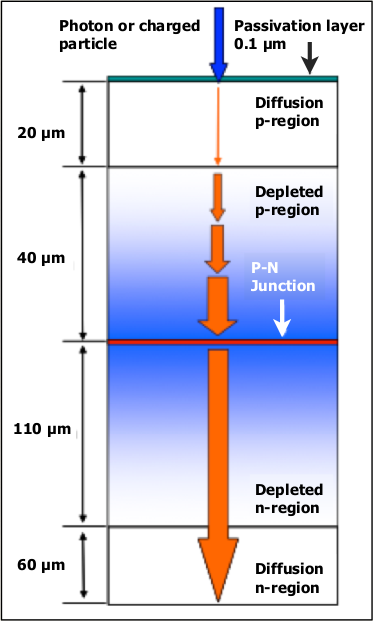
\includegraphics[width = 0.3 \textwidth, trim=0.3cm 0.3cm 0.2cm 0.3cm, clip]{APD_Diagram}}
  \hfill
  %\subfloat{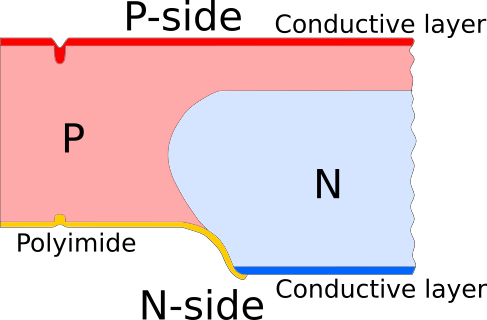
\includegraphics[width = 0.5 \textwidth]{apdSectionColorsLabels}}
  \subfloat{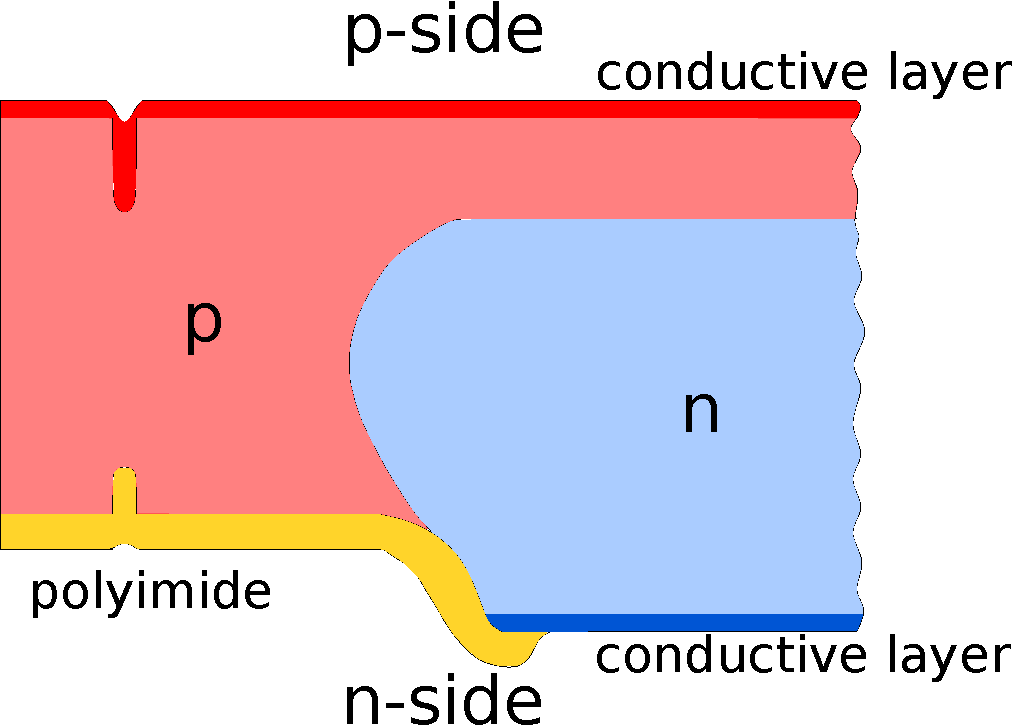
\includegraphics[width = 0.5 \textwidth]{apdSectionNew}}
  \caption{Schematic cross-sections of a deep diffused APD. {\bf Left:} centre of the detector. The thickness of the depleted region corresponds to a bias voltage of 1.8\,kV. {\bf Right:} detector edge.}
  \label{fig:apdDia}
\end{figure}

Schematic cross-sections of the centre and the edge of the resulting device are shown in figure\,\ref{fig:apdDia}.
In the following, the faces of the detectors will be referred to as p- and n-side, according to the sketch shown in figure\,\ref{fig:apdDia}.

The doping concentration of the n-type silicon is constant over the thickness of the detector, since it results from the initial doping of the silicon wafer.
The p-type silicon has a different doping profile.
As the p-type dopants are introduced through diffusion, the doping concentration of the p-type silicon is higher toward the p-side of the detector and falls toward the pn-junction.
This results in a broader peak of the electric field at the pn-junction, when compared to the triangular shape of an abrupt junction.
The broadening of the peak increases the distance over which the charge carriers drift in the highest field region, requiring a lower peak field for a given gain value.
%The broadening of peak allows the charge carriers to drift in the highest field region for a longer distance, requiring a lower peak field for a given gain value.
This reduces the ratio between the electron and hole multiplication coefficients, reducing in turn the excess noise factor due to multiplication\,\cite{theoryDDAPD}.

The applied bias voltage is usually around 1.8\,kV, resulting in a gain of up to\,500.
At this bias voltage the thickness of the depletion region is around 150\,$\mu$m.


\section{Samples and Irradiations}
\label{sec:samples}

All the APDs used in this study present the structure detailed in the previous section.
Detectors of two different sizes were used.
In this section, the geometry and readout of the different APDs are explained.

\subsection{$2 \times 2$~mm$^2$ APDs}

APDs with a nominal active area of $2 \times 2$~mm$^2$ were used to study the effects of neutron irradiation.
The dies of these devices have an area of $3.1 \times 3.1$~mm$^2$ and a circular mesa structure with a diameter of about 0.8\,mm.
These devices are mounted on ceramic supports, two metallic leads are used to contact the p- and n-sides of the detector.
The n-side of the detector faces the ceramic support.
The contact between the APD and the metal leads is achieved using conductive glue.

The $2 \times 2$~mm$^2$ APDs have a DC-coupled readout.
In order to facilitate the handling and electrical connection to the sensors, each APD was mounted on a printed circuit board (PCB) for its characterisation both before and after irradiation.
The PCB was equipped with a temperature sensor and the connectors needed to link the APD to the measuring devices.

The sensors were irradiated with neutrons at the nuclear reactor of the Jo\v{z}ef Stefan Institute in Ljubljana\,\cite{jsiIrrad}.
The fluences accumulated by the sensors ranged from $\Phi_{eq} = 3 \cdot 10^{13}$\,cm$^{-2}$ to $\Phi_{eq} = 10^{15}$\,cm$^{-2}$.
Neither bias nor cooling were applied during the irradiation, the temperature of the samples is estimated to range between 20 and 45$^\circ$C during irradiation\,\cite{vlado}.
After irradiation, the samples were stored at a temperature below $-18^\circ$C to avoid the annealing of the defects produced during irradiation.
No annealing steps were performed after irradiation, however, it is estimated that the annealing due to handling after irradiation corresponds roughly to one hour at room temperature.
%% However, the final total annealing due to the handling of the samples, and the performance of measurements at different temperatures, was estimated to be of 73 minutes at 21$^\circ$C. %% from Sofia's thesis

\subsection{$8 \times 8$~mm$^2$ APDs}

APDs with a nominal active area of $8 \times 8$~mm$^2$ were characterised in several beam tests.
The dies of these devices have an area of $10 \times 10$~mm$^2$ and a square mesa structure with 7.5\,mm sides.

%% Studies similar to the one reported in section\,\ref{sec:unif8x8laser} have shown that the amplitude of the signal produced by the sensor when illuminated by a laser depends on the distance between the point in which the sensor is struck by the laser and the point where the sensor is connected to the readout electronics.
As shown in section\,\ref{sec:unif8x8laser}, the amplitude of the signal produced by the sensor when illuminated by a laser depends on the distance between the point in which the sensor is struck by the laser and the point where the sensor is connected to the readout electronics.
This behaviour is the result of the non-negligible resistance of the conducting layers applied to the p- and n-side of the detector.

Two methods were used to improve the uniformity of response.
%% The first one, used in the devices characterised in beam tests, relies on an AC-coupled readout of the p-side of the detector.
The first one relies on an AC-coupled readout of the p-side of the detector.
A gold layer is applied to the n-side of the detector to improve its conductivity.
The electrical contact to the p-side is achieved through the formation of a bond-pad and wire-bonding.
The p-side is covered by a Kapton layer and a metallic mesh is placed above the Kapton.
The mesh picks-up the signal and provides an electrical path with a resistivity lower than the one of the conductive layer.
The sensors produced with this configuration were usually placed on PCBs containing the readout electronics.
These detectors are usually operated by applying the high voltage to the p-side and keeping the n-side at ground potential.
In this way it is possible for the electronics to directly read out both signals from the mesh and the n-side of the sensor.

Another method used to improve the uniformity of response is the metallisation of both the p- and n-side of the detector.
The metallisation consists in an aluminium deposition containing openings for laser illumination.
The detectors produced with this configuration have a DC-coupled readout and were used in laboratory tests.
These sensors were mounted on the same kind of PCBs used for the $2 \times 2$~mm$^2$ APDs, that contain a temperature sensor and the connectors to bias and readout the sensor.

In this paper detectors with both the DC-coupled mesh readout are characterised, but at the time of this writing only DC-coupled devices have been characterized after irradiation. 

%\subsection{Laboratory and Beam Test Results on Mesh Readout $8 \times 8$~mm$^2$ APDs}

%Here we summarize the basic performance characteristics of the mesh readout devices, which have now been used by us in beam tests at various facilities
%including  electron beams (DESY and LNF, Frascati) as well as low energy (PSI) and high energy (CERN PS, SPS and FNAL) pion and muon beams.
%These tests were carried out in coordination with successive improvements in device packaging and integration with a specially developed fast transimpedance 
%amplifier (need reference from Mitch) and these developments have led to improvements in response uniformity and time resolution.

%We therefore focus on the current performance of unirradiated mesh devices and will leave to a future paper the impact on timing performance which is framed
%by the radiation effects reported here- on bare devices.

%The reason that we have chosen to use a semi-transparent mesh electrode for the capacitive readout is to leave open the possibility of laser testing, which complements the charged particle response measurements.

\section{Gain Measurement of $8 \times 8$ mm$^2$ APDs using a Blue LED}
\label{sec:gain8x8led}
%The gain was measured using a red (430nm?) laser pulse impinging on the top surface (Fig.1, left). Photoelectrons released in the upper low field region then drift toward the junction
%and undergo multiplication by impact ionization (internal gain). The magnitude of this gain is set by decreasing the E-field to an asymptotically low value where multiplication stops (G=1).
%A summary of such measurements is shown in (Figure: Gain) for a range of operating temperatures. As can be seen from this figure, the Gain for a given detector bias decreases with increasing temperature.
%In fact, the data plotted in (Figure:Gain) all roughly coincide with a voltage scaling that corresponds to roughly to $\delta$V$\sim-2.45$V per deg. C.

The gain of $8 \times 8$ mm$^2$ APDs was measured using a pulsed LED.
The LED had a wavelength of 425 nm and the pulses had a duration of 20 ns.
\textcolor{red}{Readout ?}
Unity gain refers to the amplitude obtained at $\approx$500 V bias, where the amplitude shows a weak dependence on the bias voltage~$V$.
The measurements were performed at different temperatures, and the results are reported in figure\,\ref{fig:gainVsV}.
An attempt was made to parametrize
% regular trend 
the  voltage~$U$ required for a given gain as a function of temperature~$T$.
A temperature dependent shift $U' = U -2.45~ V/^\circ C \cdot \Delta T( 0^\circ C)$ describes the change in voltage necessary to normalize a given value of gain to the gain obtained at $0^\circ C$ when the the temperature of the APD is changed. Here $\Delta T( 0^\circ C)$ gives the temperature difference to $0^\circ C$. 
\textcolor{red}{What does the (0C) mean in this case? Does the shift refer to the 0C curve?
mm: ...take a look if this is now formulated as meant??} The result of this scaling law is shown in figure \ref{fig:gainVsV}(Right).
%This parametrization of the pattern up to a gain of 
It describes the data up to a gain of
$\approx$1000 and may prove useful for discriminating among impact ionization models that appear in the literature and as options in TCAD\footnote{Technology Computer Aided Design.} software for modeling such devices.
It should be noted that this particular definition of gain, as it applies to visible light photodetection in an APD, 
%will likely differ 
is different from the gain obtained from the response to minimum ionizing particles (or the IR laser model used) since, in the former case all photoelectrons traverse the region where impact ionization occurs.
\textcolor{red}{Another difference could be the focusing? Was the light focussed? Which was the intensity?}
\textcolor{red}{We need to refer to our other gain definitions here.}

\begin{figure}
  \centering
  \subfloat{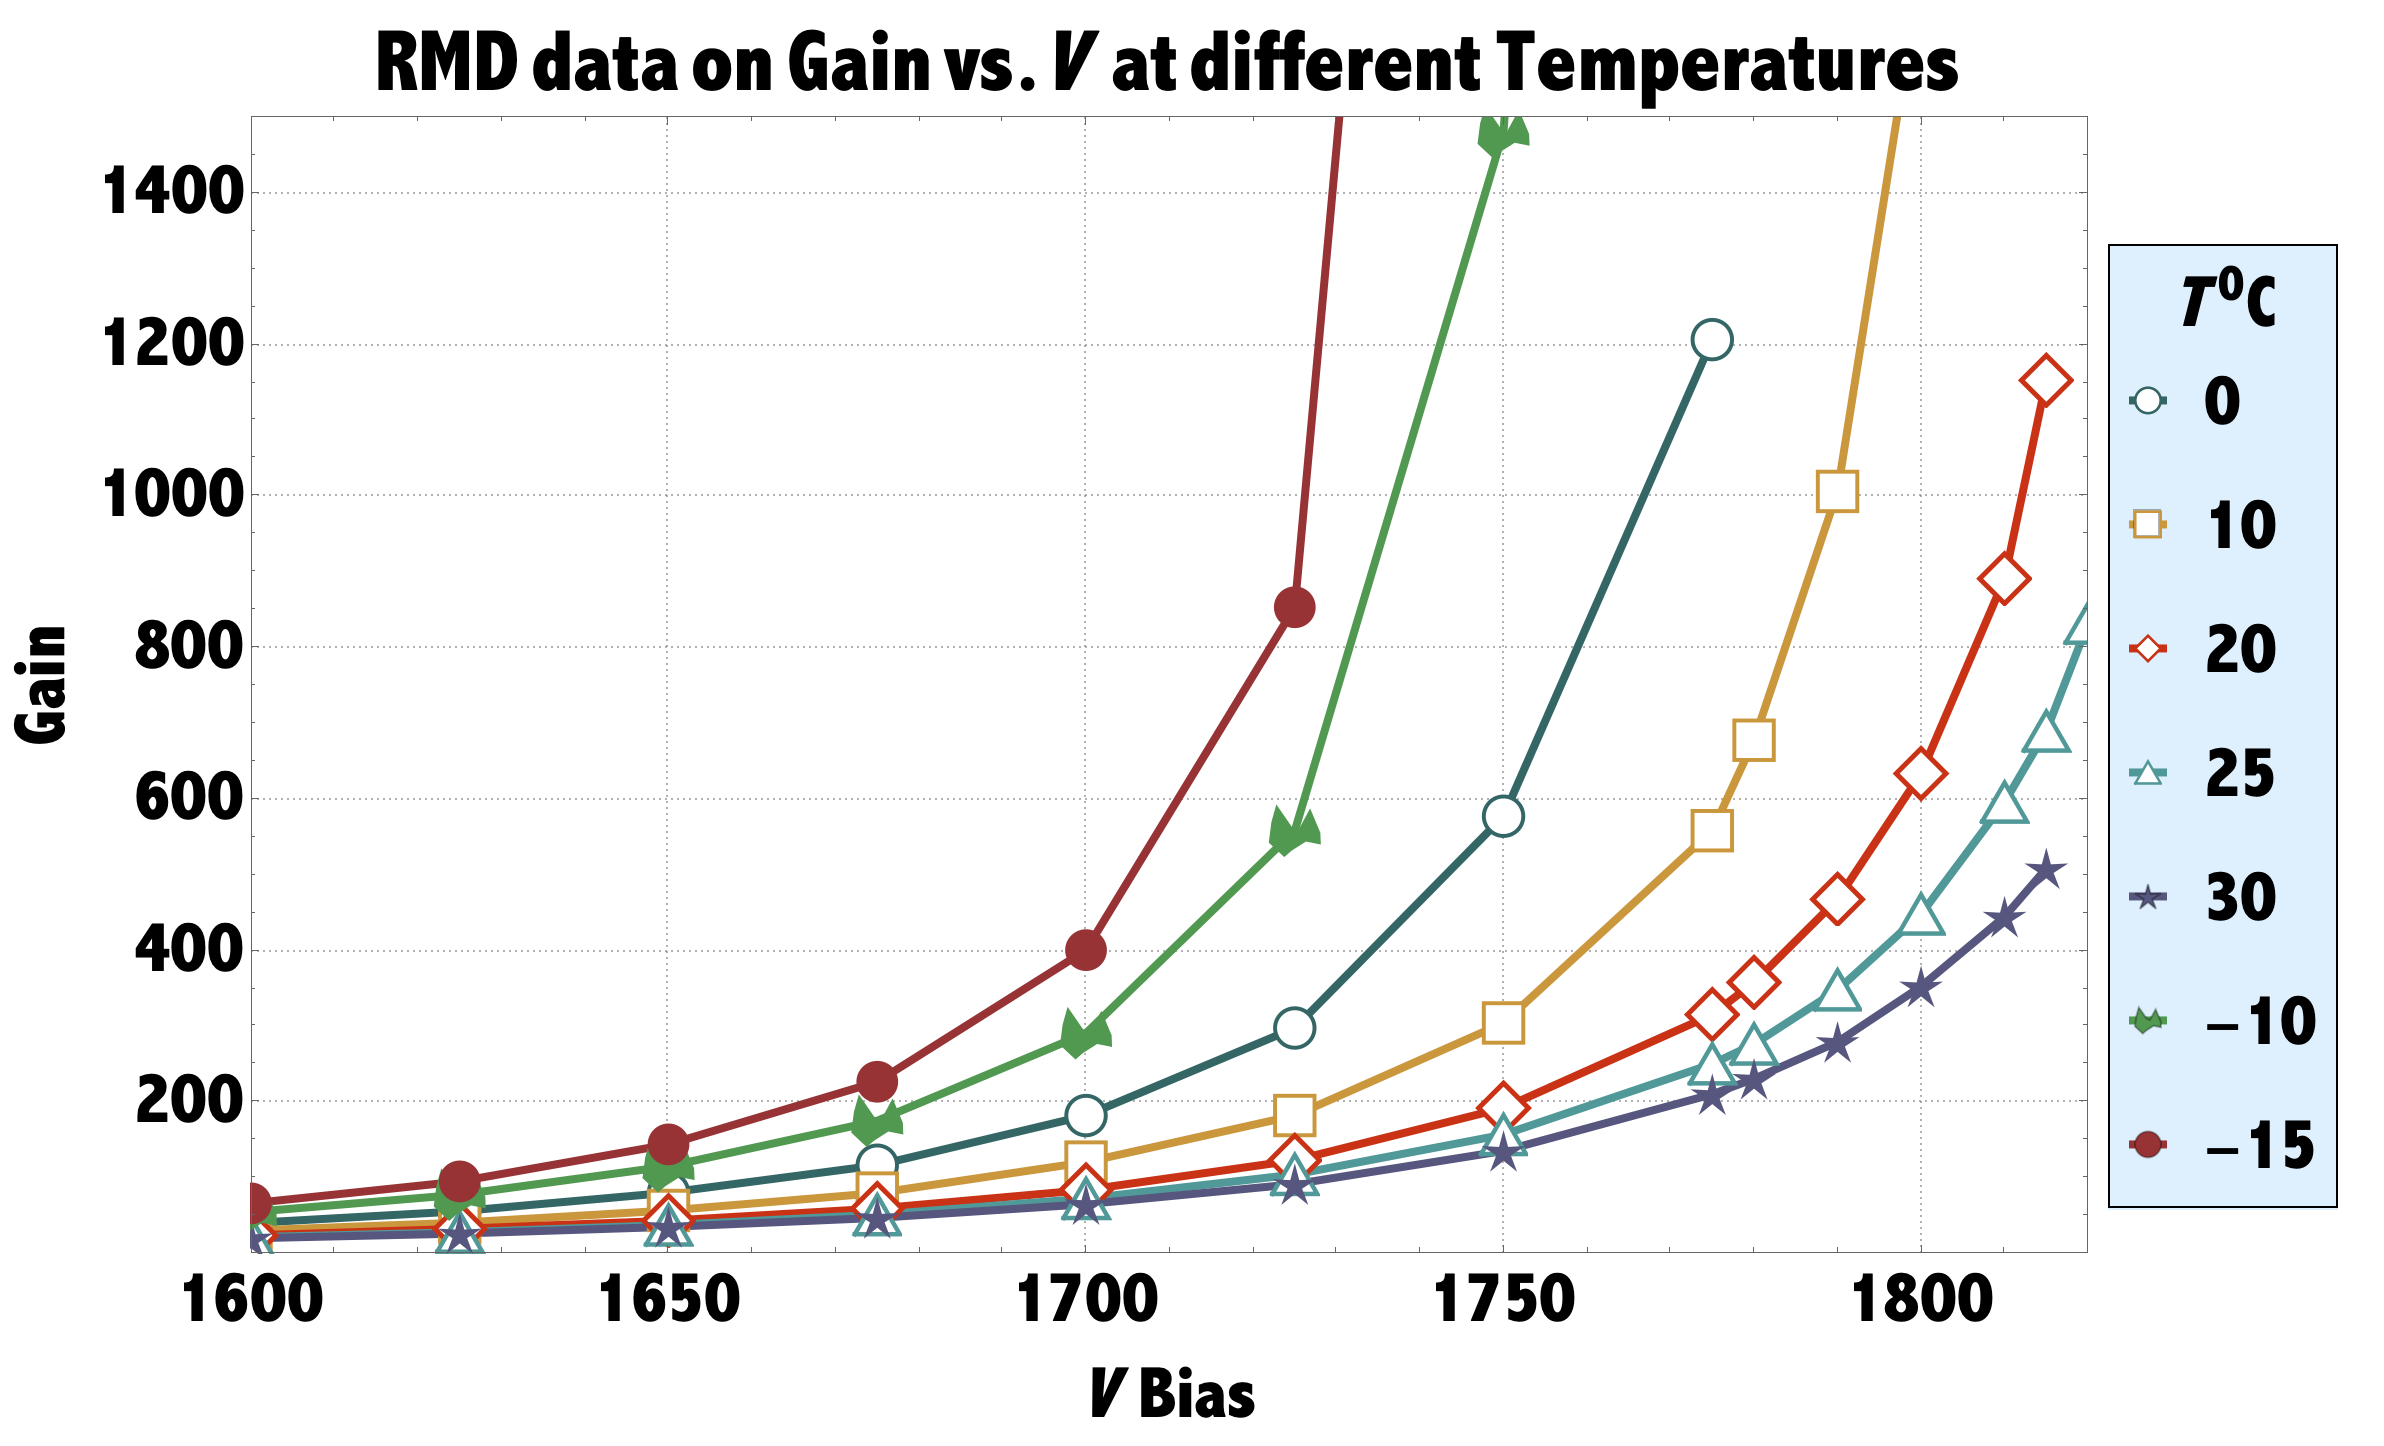
\includegraphics[width = 0.55 \textwidth]{gainVsV}}
  \hfill
  \subfloat{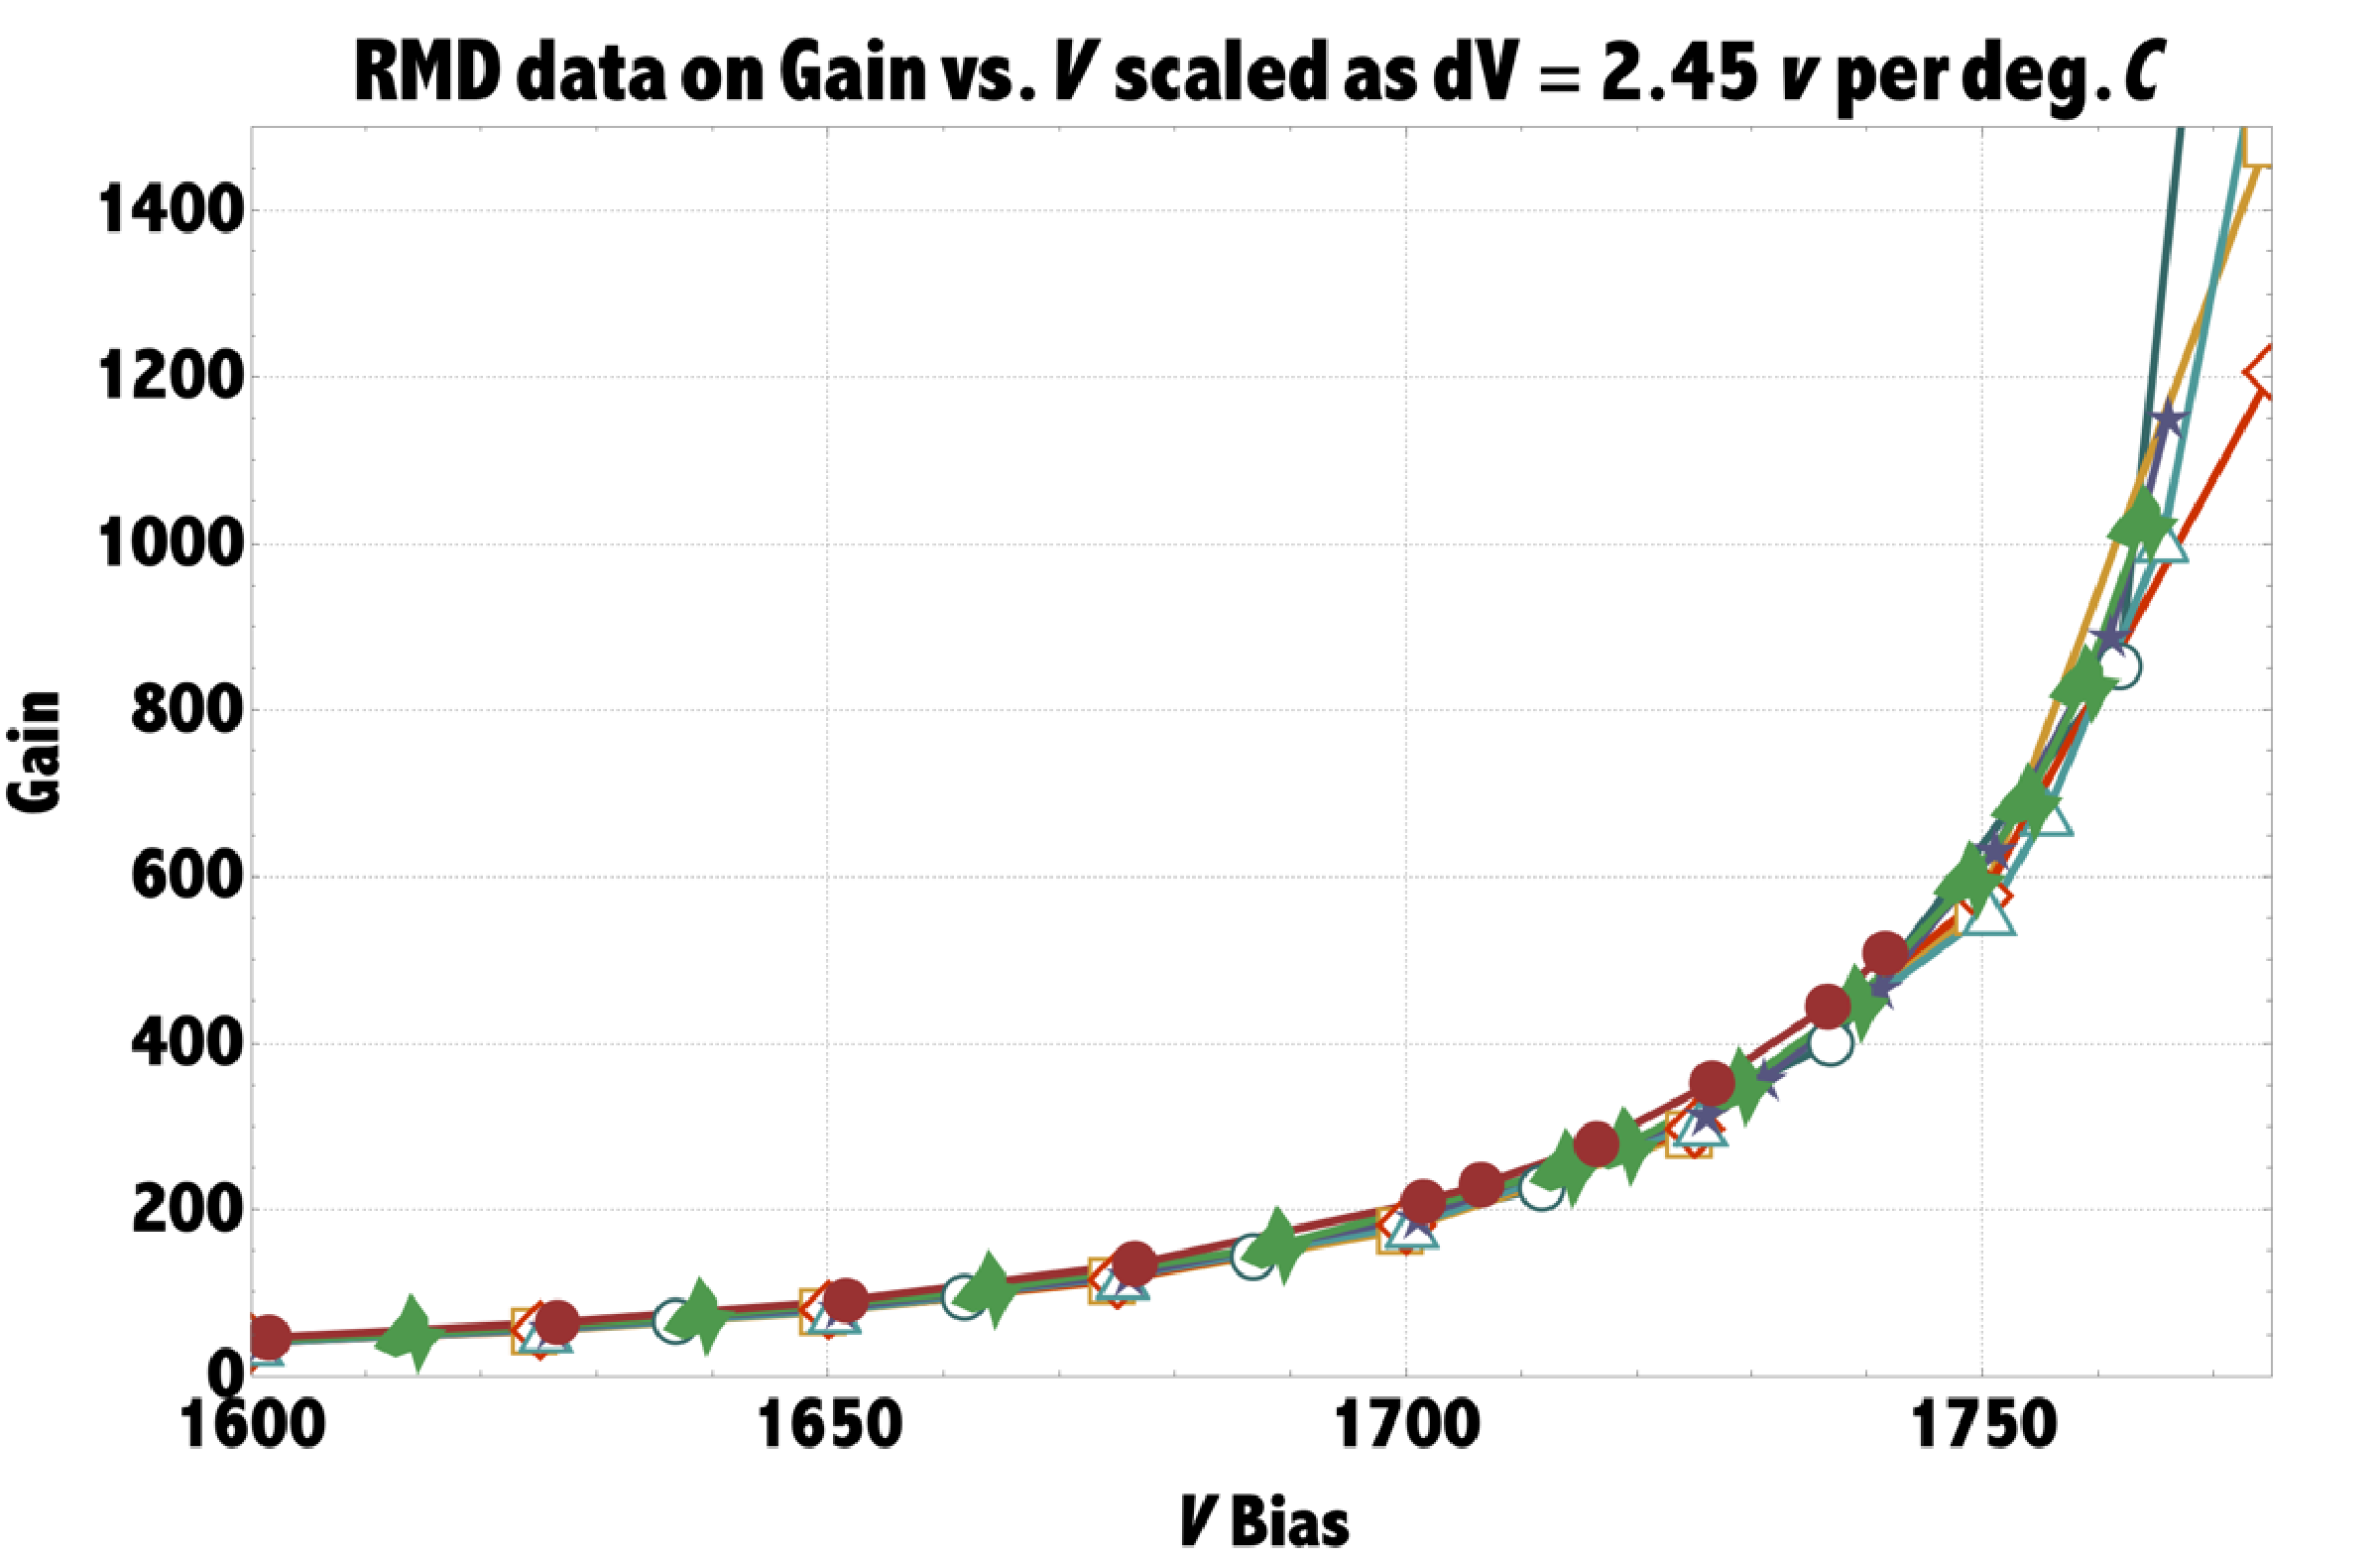
\includegraphics[width = 0.45 \textwidth]{gainVsVscaled}}
  \caption{\textbf{Left:} Gain of a $8 \times 8$ mm$^2$ APDs as a function of bias voltage at different temperatures. The measurement was performed using a blue LED. \textbf{Right:} By shifting the bias for each curve according to the law described in the text, a scaling law is found.}
  %\label{fig:gainfig}
  \label{fig:gainVsV}
\end{figure}

\section{Laboratory Characterisation of Irradiated $2 \times 2$~mm$^2$ APDs}
\label{sec:irrad2x2}

\subsection{Experimental Methods}

Two experimental setups were used to characterise the APDs.

The current-voltage characteristic of the detectors was measured using a voltage source and a picoammeter connected in series to the sensor under test.
The sensor was placed inside a climate chamber flushed with dry air where the temperature could be controlled.
The temperature sensor on the PCB was used to ensure that the APD reached thermal equilibrium with the air in the climate chamber before starting the measurements.

The response of the APDs to a pulsed infrared laser was measured in a different setup and used to determine the variation of the sensor's signal and time resolution as a function of bias voltage and irradiation fluence.
The laser has a wavelength of 1064\,nm and the pulses have a duration of 200\,ps.
The repetition rate was chosen to be 200\,Hz.
The intensity of the light impinging on the APD was determined to correspond to a charge deposition in the sensor of 15 or 0.8\,MIPs per pulse, depending on the measurement.
A shutter is used to change the light intensity.
The amount of deposited charge per laser pulse was measured using a non-irradiated pad diode of known thickness.
The charge deposited for one MIP is defined as 74 electron hole pairs per micron of silicon.
The wavelength used has an absorption length in silicon of about 1\,mm, resulting in the generation of electron hole pairs through the whole sensor thickness.
The light pulses are propagated from the laser to the sensor through an optical fibre.
A coupler diverts part of the light to a photodiode that is used to monitor the intensity of the light pulses.
An optical system focuses the light on the sensor surface producing a beam spot of about 15\,$\mu$m in diameter.
The bias voltage of the sensor under test is provided by a voltage source containing a picoammeter used to monitor the current flowing through the sensor.
The temperature of the APD was controlled using a cooling system constituted by a Peltier element and a chiller.
The temperature measured by the temperature sensor on the PCB was used as input to the Peltier control system.
The APD was housed in a light-tight Faraday cage flushed with dry air during the measurements.
The APD signal was amplified using a CIVIDEC C2HV broadband amplifier\,\cite{cividec}.
Both the signals of the APD and the photodiode were digitised using an oscilloscope with 2.5\,GHz bandwidth and a sampling rate of 20\,GSa/s.

For the measurement of the APD signal amplitude and uniformity of response, an amplification of 10\,dB was used, together with a light intensity corresponding to 15\,MIPs.
This amplification was achieved by attenuating the APD signal with a 30\,dB attenuator and then amplifying it with a 40\,dB amplifier.
The 40\,dB amplifier is the same used in the time resolution measurements.
The reduction of the gain to 10\,dB is necessary in order to perform the amplitude measurements over the desired bias voltage range while remaining in the amplifier's linear range.
For each measurement condition, the waveforms were averaged 256 times in the oscilloscope before being stored for analysis.

The time resolution measurements were performed applying a 40\,dB amplification to the APD signal.
No averaging was applied to the waveforms.
A gain of 40\,dB provides a better signal to noise ratio for the APD signal, compared to the 10\,dB used for the amplitude measurement.
The intensity of the light shone on the APDs for these measurements corresponded to 0.8\,MIPs.
The optical system was modified for the timing measurements.
A splitter and delay line system was introduced, allowing to shine two light pulses on the sensor for each pulse generated by the laser.
The system is realised using optical fibre, and consisted of a splitter, a short and a long optical fibre branch, and a merger.
The difference in length between the two branches corresponds to a delay of 50\,ns between the pulses.
The sensor's signals from the light pulses were digitised in the same waveform in the oscilloscope.
The difference in the amplitude of the two signals was below 5\%.
Given the similar amplitude, the signals can be used to determine the time resolution of the detector under test, without the need of an external timing reference.

The APD temperature was $-20^\circ$C during all measurements reported in this section.
For the measurements of intensity as a function of bias voltage and the timing measurements using the laser, the light was shone on the centre of the APDs.

\subsection{Results}

\begin{figure}
  \centering
  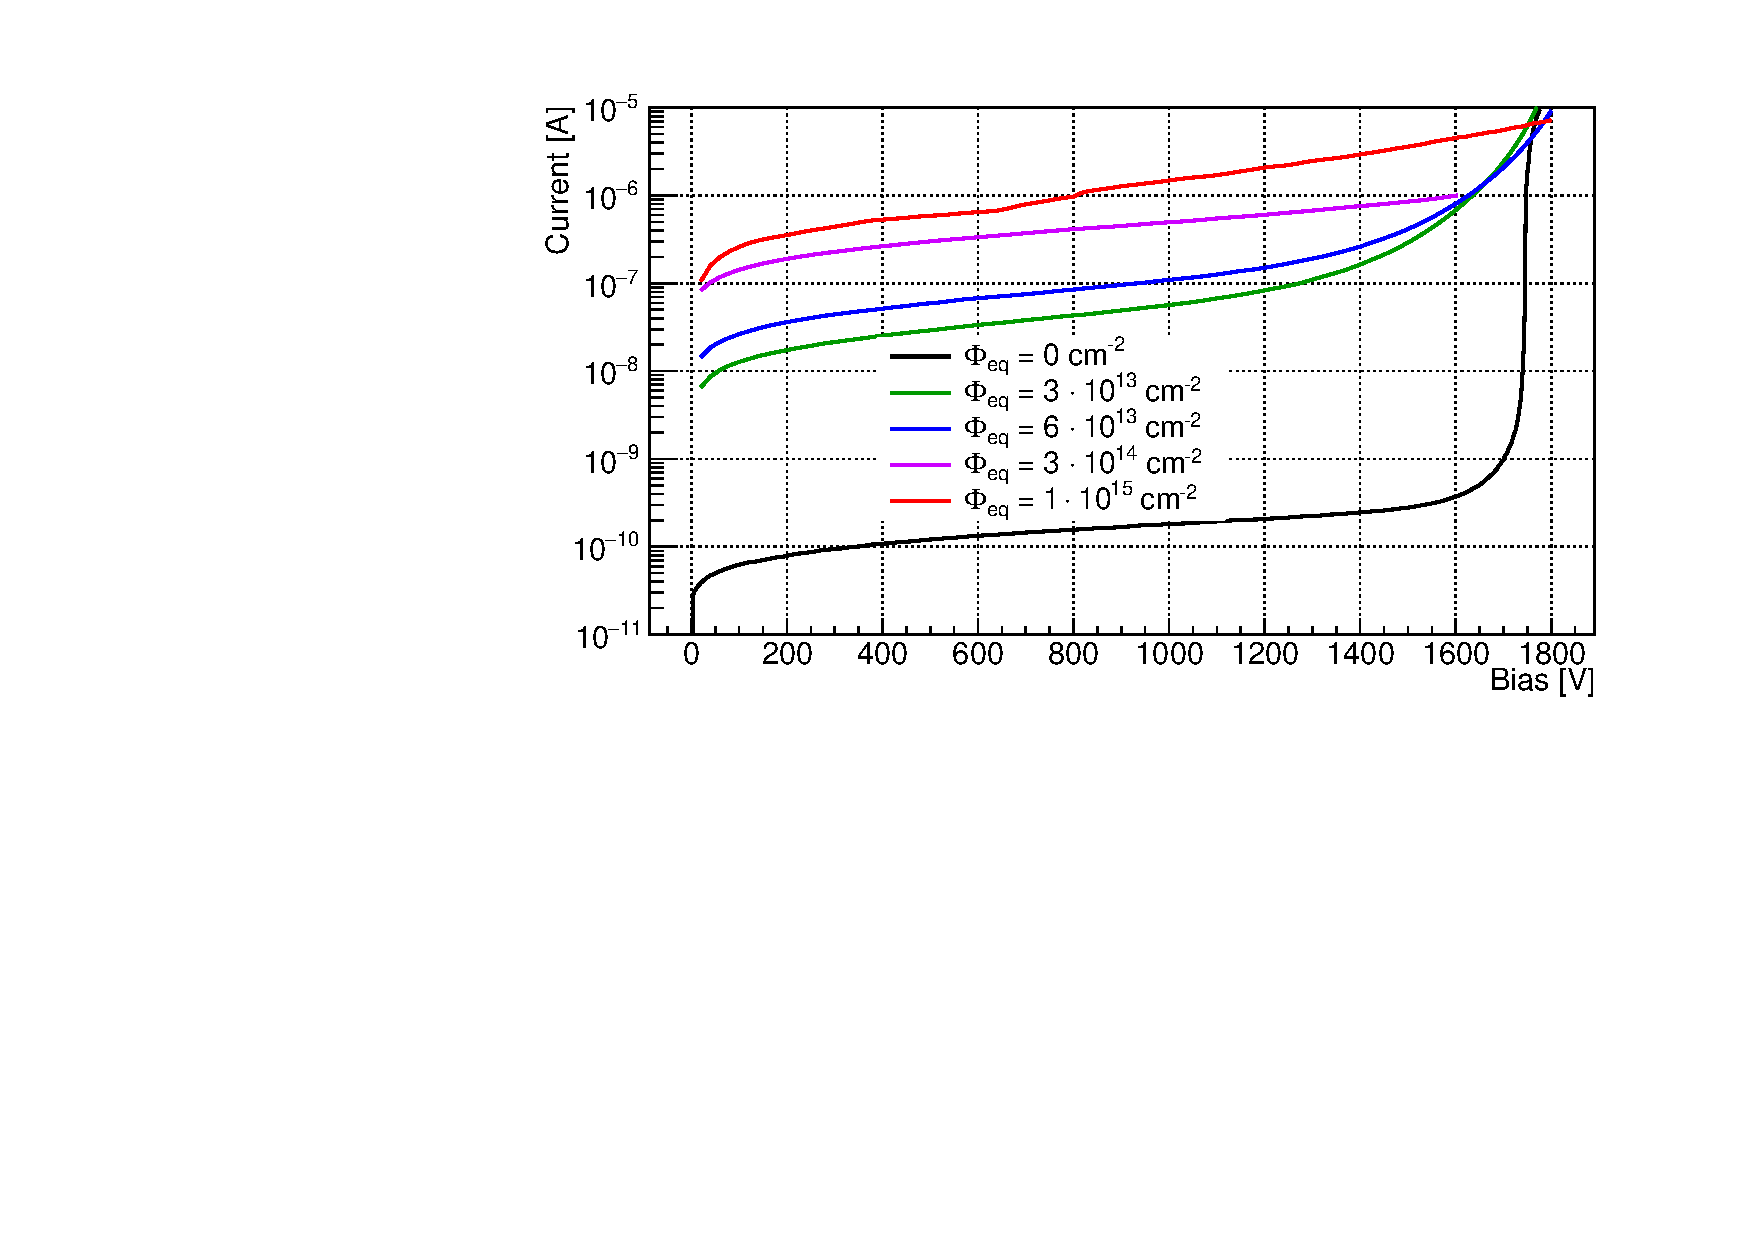
\includegraphics[width = 0.6 \textwidth]{IVnIrrad}
  \caption{Current-voltage characteristics of the $2 \times 2$~mm$^2$ APDs measured at $-20^\circ$C for different neutron fluences.}
  \label{fig:iv2x2}
\end{figure}

\paragraph{Current-voltage characteristic}
The current-voltage (IV) characteristic of the APDs is shown, for different fluences, in figure\,\ref{fig:iv2x2}.
Before irradiation, below 1600\,V, the current assumes a value of less than a few nA.
In this region the main contribution to the current is thought to be surface current.
Between 1600 and 1800\,V, the current increases by 4 orders of magnitude.
This is the region where the multiplication dominates the IV characteristic of the non-irradiated sensors.
The surface current is not affected by multiplication, therefore the multiplication of bulk current in the non-irradiated sensors can not be seen in the IV curve until the gain is sufficiently high.

The irradiation enhances the bulk generation current of the devices, as can be seen in the region between 0 and 1200\,V, where the gain of the sensors does not influence the curves.
As the bulk current is amplified, the shape of the irradiated sensors' curves is different from that of the non-irradiated sensor.
The change in the magnitude of the current at high voltages is different with respect to the non-irradiated sensor, suggesting that the gain of the detectors is reduced by irradiation, or respectively that a higher bias voltage is required to obtain the same gain as for the non-irradiated sensor.

The current related damage rate ($\alpha$) was estimated at 200\,V, where no multiplication is expected.
Under the assumption that the depleted volume at this voltage does not change with irradiation, the measured value of $\alpha$ is of the expected order of magnitude.

The sensor irradiated to $\Phi_{eq} = 3 \cdot 10^{14}$\,cm$^{-2}$ shows a breakdown around 1600\,V, therefore no information about its IV characteristic is available at higher bias voltages.
This also applies to the amplitude measurements presented below.

\begin{figure}
  \centering
  \subfloat[$\Phi_{eq} = 0$\,cm$^{-2}$, 1700\,V]{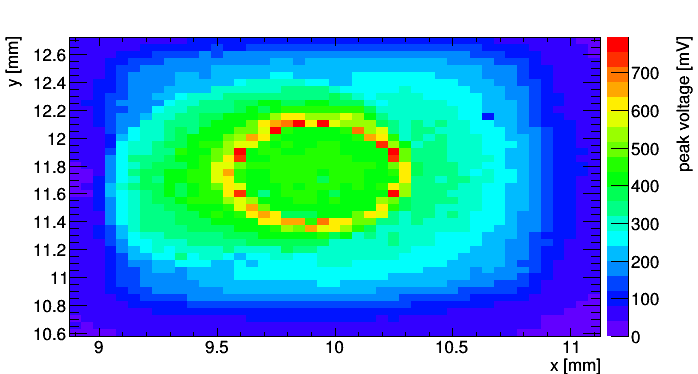
\includegraphics[width = 0.45 \textwidth]{APD_2B_3_IR_XY_peak_scan_m20C}}\\
  \subfloat[$\Phi_{eq} = 3 \cdot 10^{13}$\,cm$^{-2}$, 1679\,V]{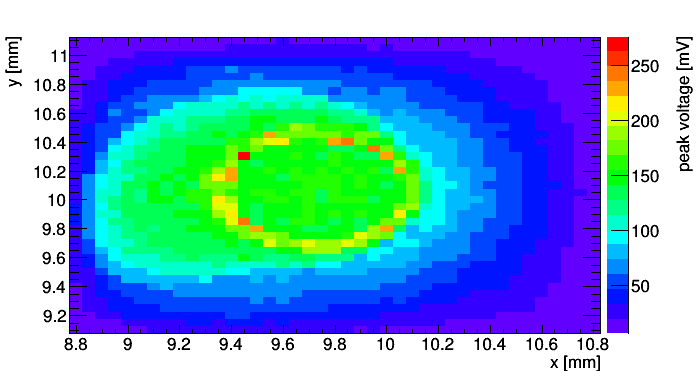
\includegraphics[width = 0.45 \textwidth]{APD_2B_3_IR_XY_peak_scan_m20C_3E13}}\hfill
  \subfloat[$\Phi_{eq} = 6 \cdot 10^{13}$\,cm$^{-2}$, 1673\,V]{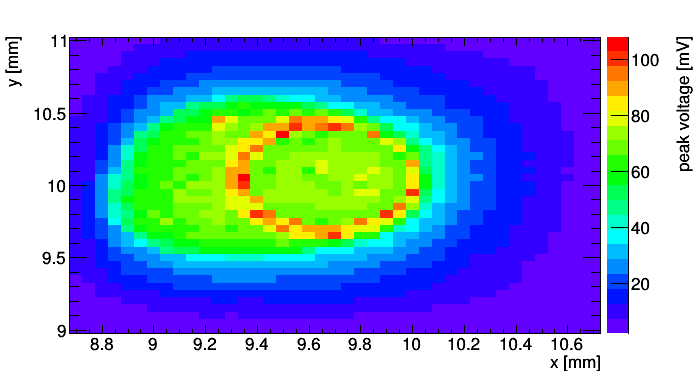
\includegraphics[width = 0.45 \textwidth]{APD_2B_5_IR_XY_peak_scan_m20C_6E13}}\\
  \subfloat[$\Phi_{eq} = 3 \cdot 10^{14}$\,cm$^{-2}$, 1677\,V]{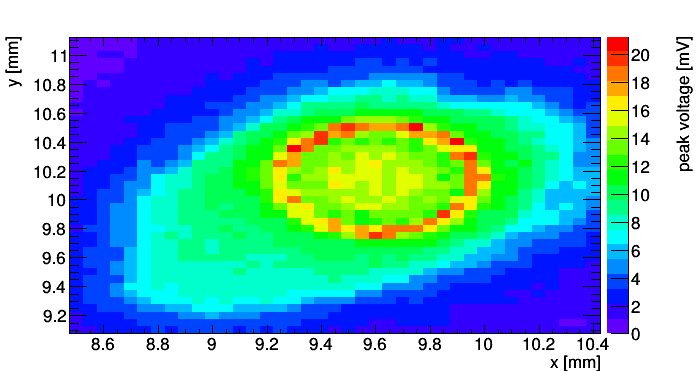
\includegraphics[width = 0.45 \textwidth]{APD_2B_4_IR_XY_peak_scan_m20C_3E14}}\hfill
  \subfloat[$\Phi_{eq} = 10^{15}$\,cm$^{-2}$, 1644\,V]{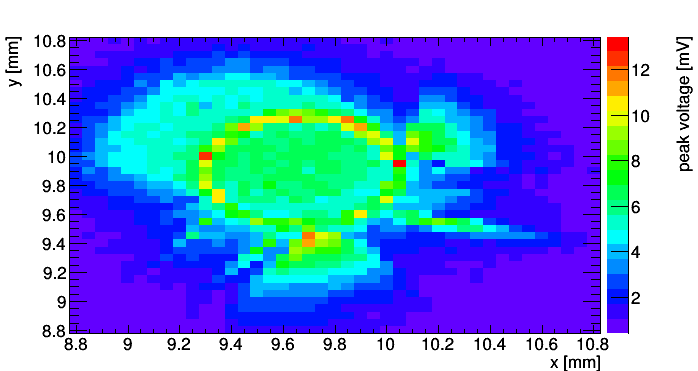
\includegraphics[width = 0.45 \textwidth]{APD_2B_9_IR_XY_peak_scan_m20C_1E15}}
  \caption{Signal amplitude as a function of the position where the laser was focused on the sensors measured at $-20^\circ$C. The laser intensity corresponds to 15\,MIPs. An amplification of 10\,dB was used.}
  \label{fig:xyScanIR_2x2}
\end{figure}

\paragraph{Uniformity of response}
The uniformity of response was measured using an infrared laser with pulses of an intensity corresponding to 15\,MIPs and an amplification of 10\,dB.
The laser was focused on different parts of the sensors and the average of 256 waveforms was stored and the signal amplitude extracted.
The signal amplitude as a function of position of the laser spot on the sensors is shown in figure\,\ref{fig:xyScanIR_2x2}.
The difference in the bias voltage applied to the detectors is due to the current drawn by the detectors under bias.
The biasing and readout circuit had a total resistance of 13\,M$\Omega$ connected in series to the sensor under test.
The bias voltage applied to the readout circuit was 1700\,V for all samples, the difference in voltage from this value are due to the potential drop caused by the sensors' dark current flowing through the 13\,M$\Omega$ load.
All the values of bias voltage presented in the following take into account this effect.

The sensor irradiated to $\Phi_{eq} = 3 \cdot 10^{14}$\,cm$^{-2}$ could be biased at a higher voltage with respect to the IV measurement.
This is probably a consequence of the annealing of the radiation damage of the detector, due to handling and measurements performed at room temperature, since the measurement shown in figure\,\ref{fig:xyScanIR_2x2} were performed after the current-voltage and amplitude measurements.
This suggests that the annealing status of the detectors can influence their breakdown behaviour.

The amplitude is higher at lower $x$ values, regardless of the fluence.
This effect, although not fully understood for these devices, is thought to be similar in origin to the one studied in section\,\ref{sec:unif8x8laser} for APDs with an active area of $8 \times 8$~mm$^2$.
In each plot of figure\,\ref{fig:xyScanIR_2x2}, a circular region with increased amplitude is present.
This region corresponds to the mesa structure in the back of the devices.
Part of the light from the laser is reflected from the curved surface of the mesa toward the active area of the detectors, resulting in an increased signal.
The sensitive area of the detectors is affected by irradiation.
However, the response of the detectors appears uniform close to the detector centre, in the area enclosed by the mesa structure.
The measurements shown in the rest of this section were performed by shining the light in the centre of the detectors.

\begin{figure}
  \centering
  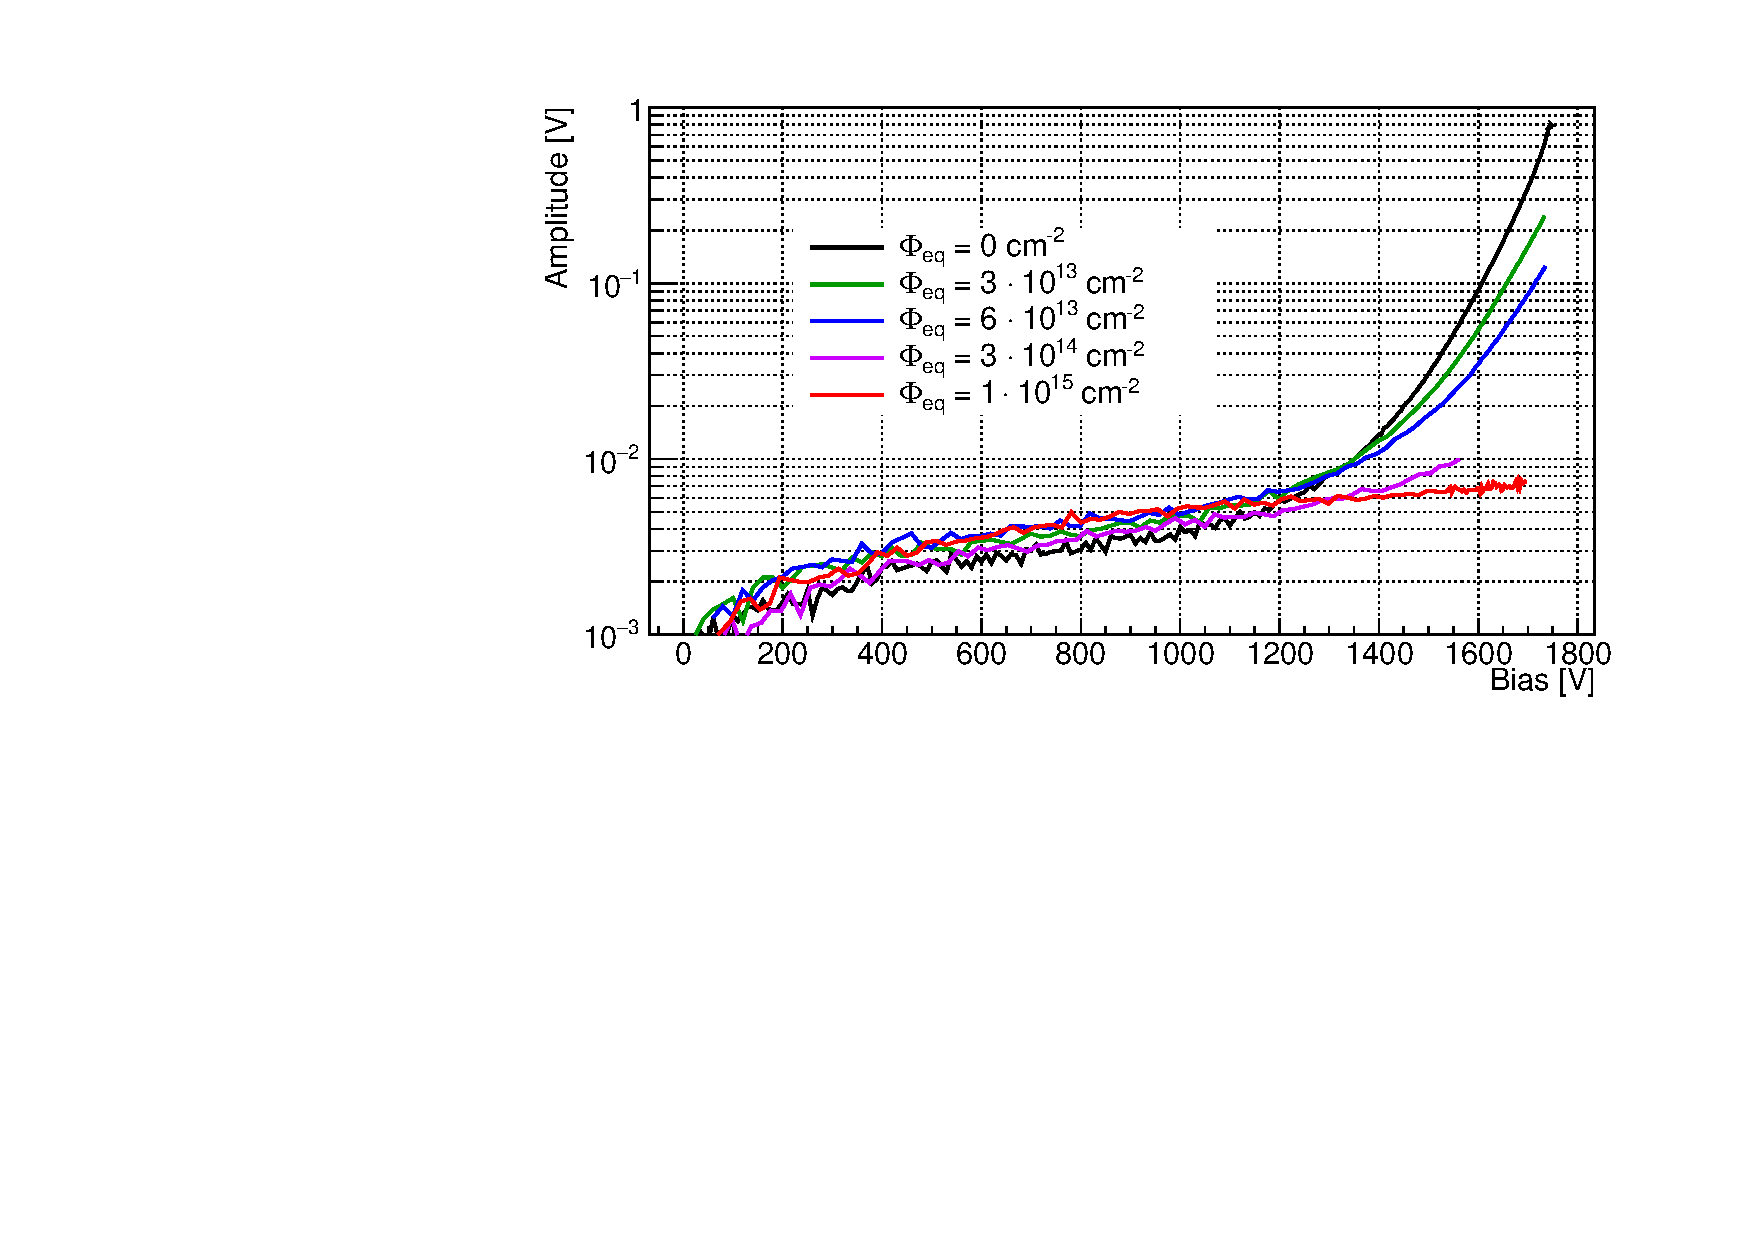
\includegraphics[width = 0.6 \textwidth]{ampliIrrad_5mV}
  \caption{Amplitude of the APDs signal as a function of bias voltage and fluence measured at $-20^\circ$C. The laser intensity corresponds to 15\,MIPs. An amplification of 10\,dB was used.}
  \label{fig:ampli2x2_15MIP}
\end{figure}

\paragraph{Signal amplitude}
The amplitude was measured from the baseline of the pulse, calculated using the part of the waveform preceding the laser pulse.
The results are shown in figure\,\ref{fig:ampli2x2_15MIP} as a function of bias voltage and fluence.

The measured amplitudes present similar values up to 1200\,V, for all the fluences.
For voltage values above 1200\,V, the signal amplitude decreases with increasing fluence, indicating a reduction of the gain for the irradiated detectors.
The behaviour of the detectors indicates that for fluences at least up to $\Phi_{eq} = 6 \cdot 10^{13}$\,cm$^{-2}$ the gain of the detectors could be recovered by applying a higher bias voltage.

\paragraph{Time resolution}
The time resolution of the sensors was determined using an infrared laser focused on the detector centre.
An optical system was used to have two light pulses shine on the sensor under test for each pulse produced by the laser.
A waveform corresponding to one laser pulse is shown in figure\,\ref{fig:pulses2x2timing}.
The amplification used for the time resolution measurements was 40\,dB, and no averaging was applied to the waveforms.
2000 waveforms were acquired for each measurement condition.

\begin{figure}
  \centering
  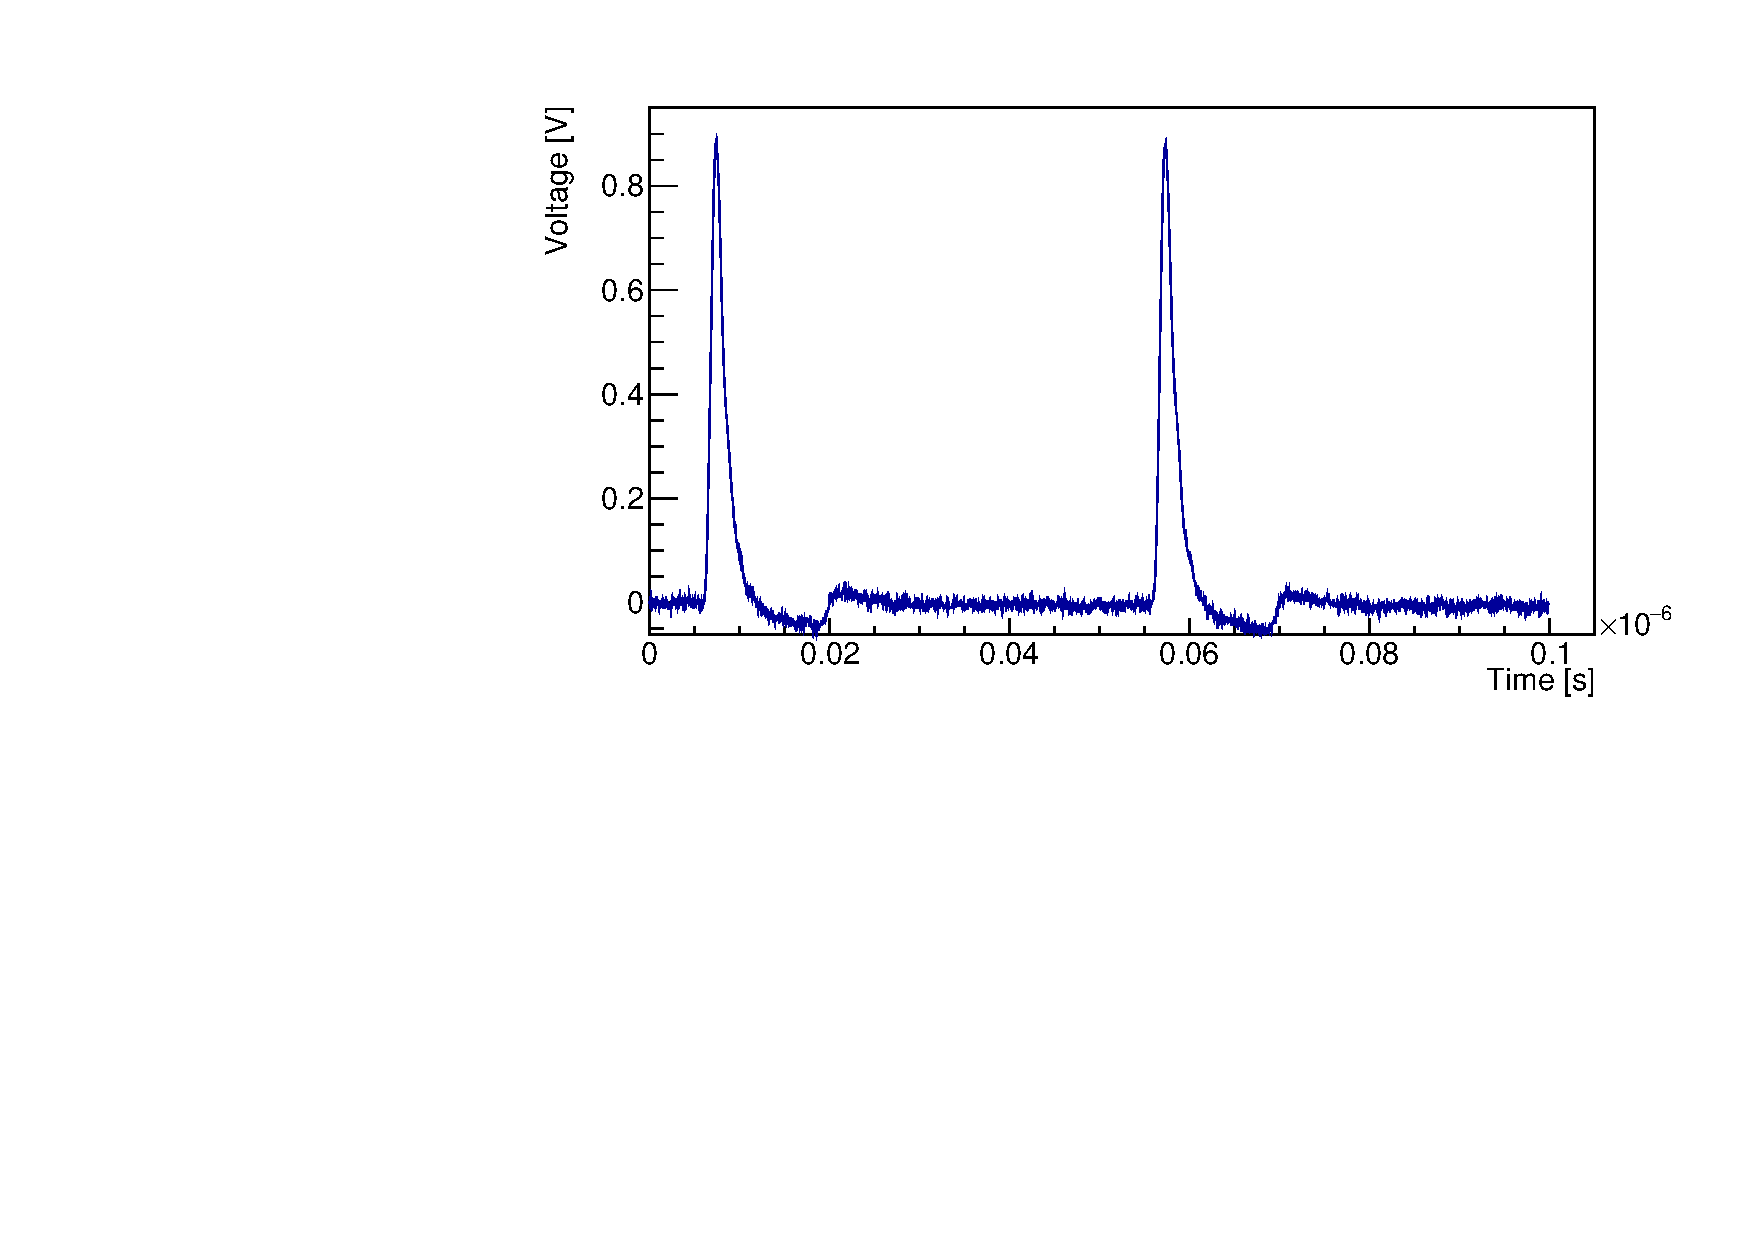
\includegraphics[width = 0.6 \textwidth]{APD_394-1-51_1665V_evt1100_2pulses}
  \caption{Waveform from a non-irradiated $2 \times 2$~mm$^2$ APD biased at 1665\,V operated at $-20^\circ$C. The laser intensity corresponds to 0.8\,MIPs. An amplification of 40\,dB was used.}
  \label{fig:pulses2x2timing}
\end{figure}

The average signal amplitude as a function of bias voltage and fluence is shown in figure\,\ref{fig:ampli2x2}.
The amplitude is limited by two components of the experimental setup.
The limiting factor for the non-irradiated sensor is the amplifier, that has a linear range corresponding to an output amplitude of $\pm 1$\,V.
For the irradiated sensors, the maximum current provided by the high voltage power supply was reached, limiting the gain achieved by the devices.
The difference between the amplitude of the two signal peaks present in each waveform was less than 5\% for each measurement.
The time resolution of the sensor irradiated to $\Phi_{eq} = 3 \cdot 10^{14}$\,cm$^{-2}$ was not measured due to its breakdown behaviour that poses a risk to the electronics used in these measurements.

\begin{figure}
  \centering
  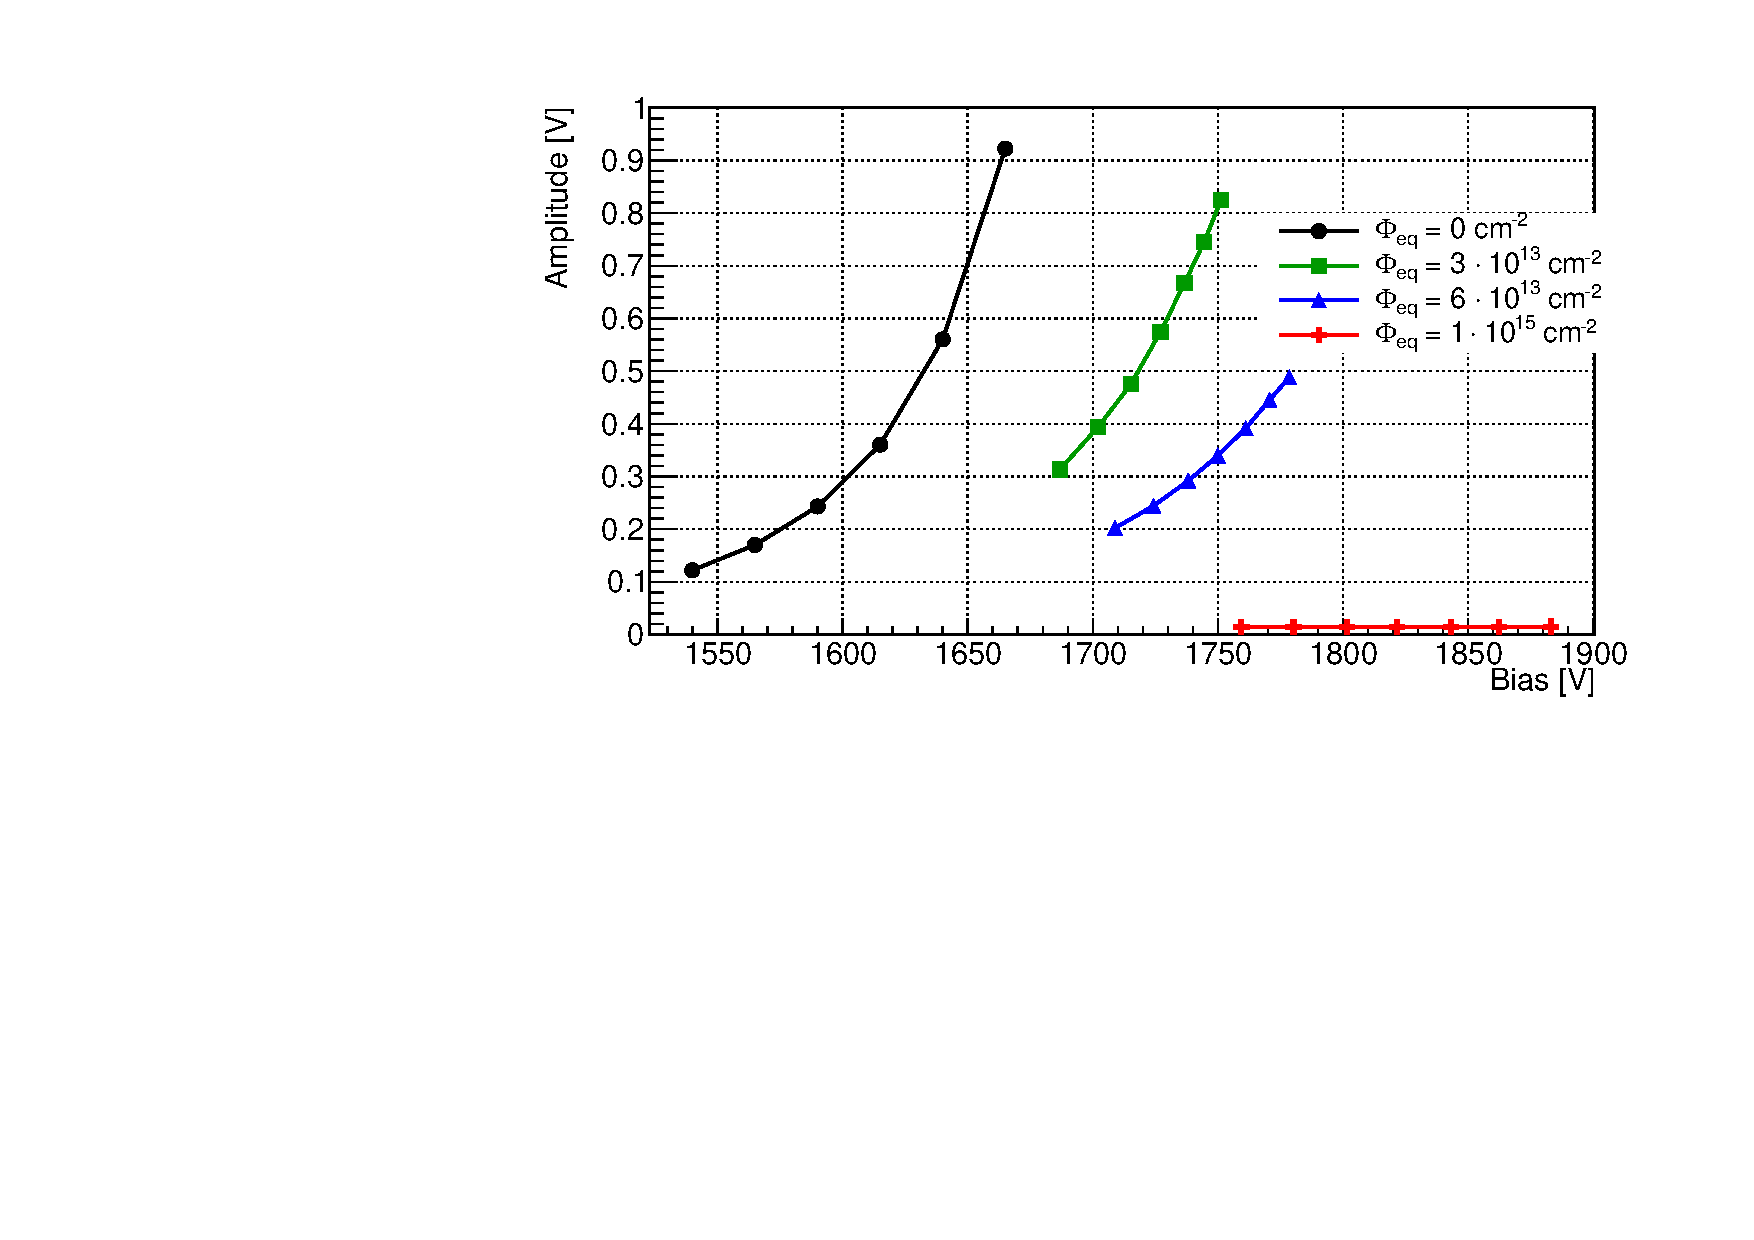
\includegraphics[width = 0.6 \textwidth]{ampli2x2APDs}
  \caption{Average amplitude of the $2 \times 2$~mm$^2$ APDs signal as a function of bias voltage and fluence measured at $-20^\circ$C. The laser intensity corresponds to 0.8\,MIPs. An amplification of 40\,dB was used.}
  \label{fig:ampli2x2}
\end{figure}

The noise is defined as the standard deviation of the distribution of the waveform points around the baseline, for the portion of the waveform preceding the pulse due to laser illumination.
The noise of the APDs, as a function of bias voltage and irradiation fluence, is shown in figure\,\ref{fig:noise2x2}.
The noise of the APDs with $\Phi_{eq} \leq 6 \cdot 10^{13}$\,cm$^{-2}$ shows a stronger dependence on the applied bias voltage than the the detector irradiated to $\Phi_{eq} = 10^{15}$\,cm$^{-2}$.
This suggests that the multiplication mechanism affects the noise of the sensors.

\begin{figure}
  \centering
  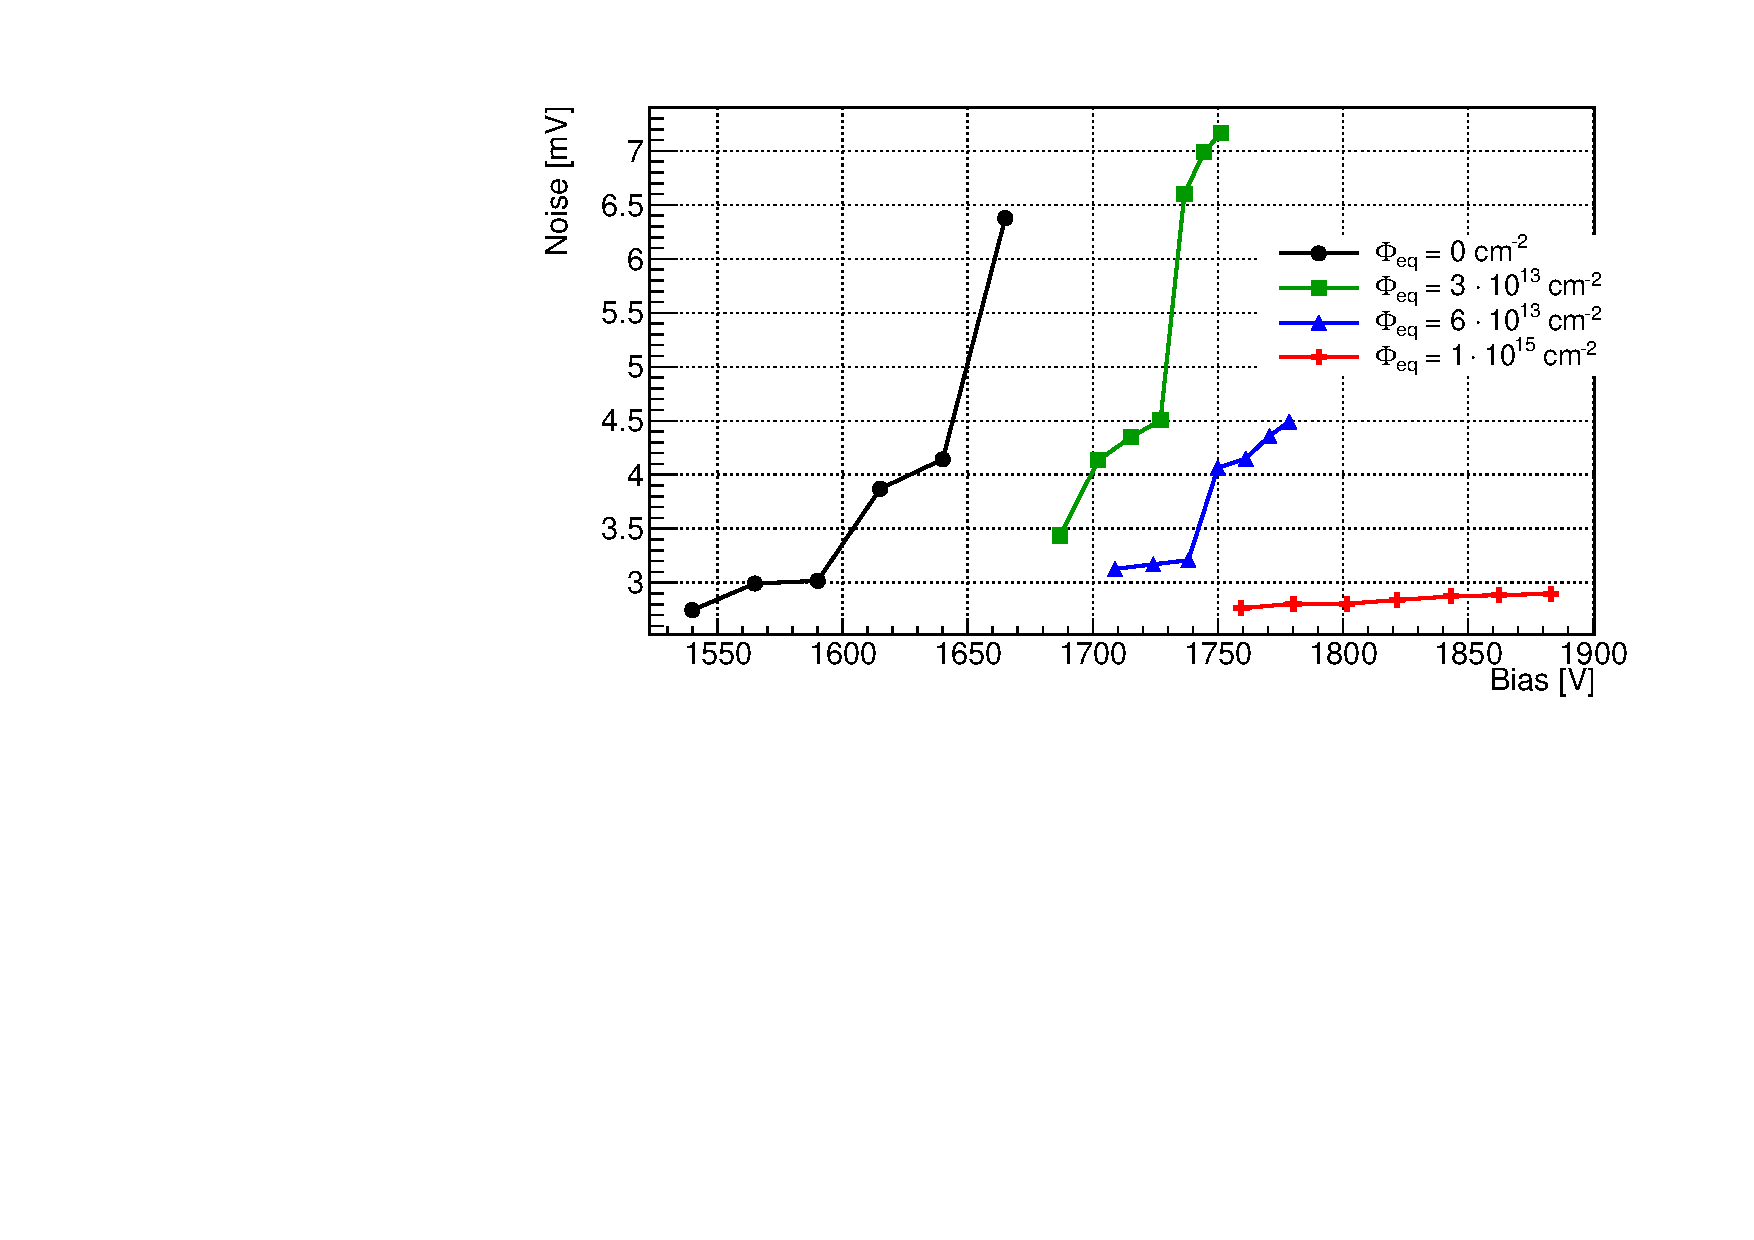
\includegraphics[width = 0.6 \textwidth]{noise2x2APDs}
  \caption{$2 \times 2$~mm$^2$ APDs' noise as a function of bias voltage and fluence measured at $-20^\circ$C. An amplification of 40\,dB was used.}
  \label{fig:noise2x2}
\end{figure}

The signal to noise ratio (SNR) is defined as the ratio between amplitude and noise and is shown in figure\,\ref{fig:snr2x2}.
The SNR is not a monotone function of the applied bias voltage.
The sensor irradiated to $\Phi_{eq} = 10^{15}$\,cm$^{-2}$ shows a weaker dependence of SNR on bias voltage than the other sensors.
This is attributed to the lower value of gain of this sensor compared to the others.

\begin{figure}
  \centering
  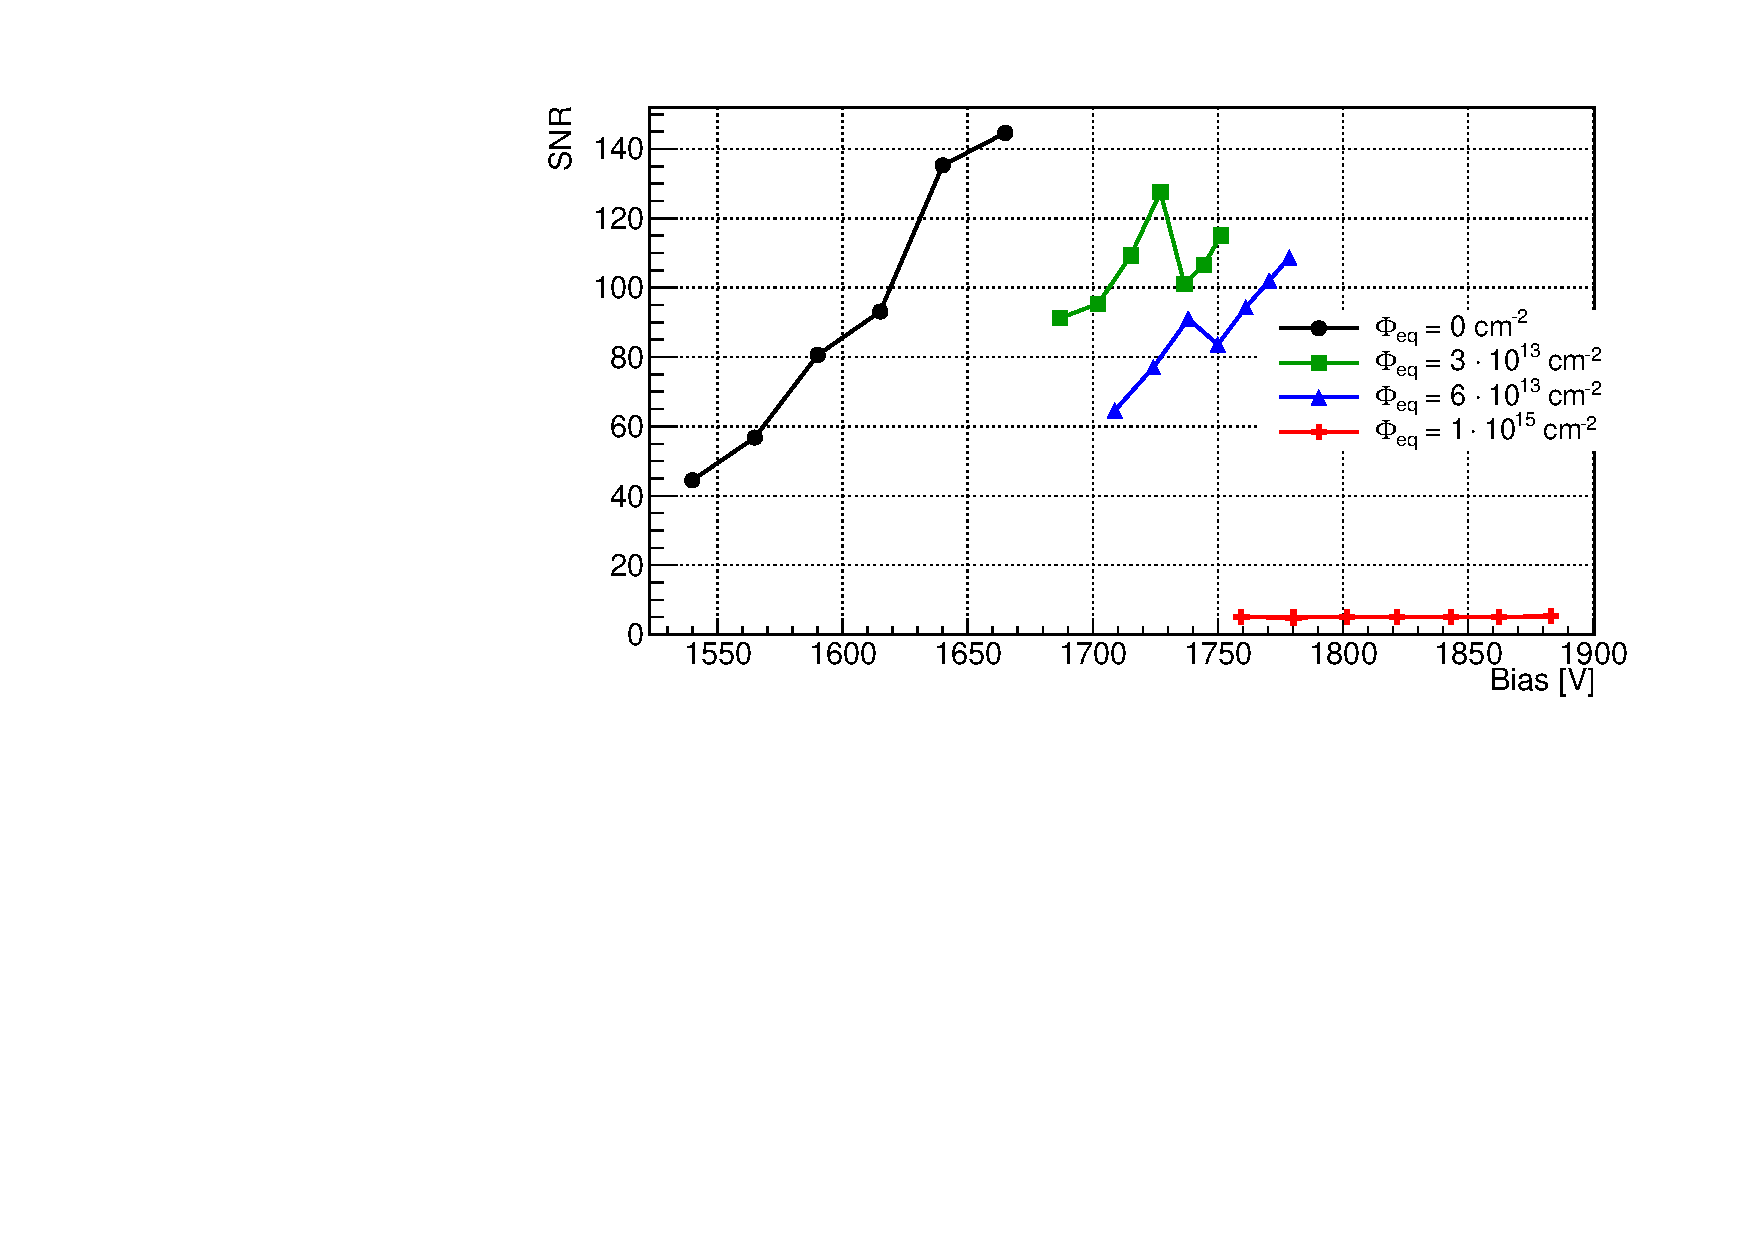
\includegraphics[width = 0.6 \textwidth]{snr2x2APDs}
  \caption{Signal to noise ratio of the $2 \times 2$~mm$^2$ APDs as a function of bias voltage and fluence measured at $-20^\circ$C. The laser intensity corresponds to 0.8\,MIPs. An amplification of 40\,dB was used.}
  \label{fig:snr2x2}
\end{figure}

The average 20\%-to-80\% rise time of the sensors is shown in figure\,\ref{fig:riseTime2x2}.
The crossing time of the 20\% and 80\% thresholds was determined using a linear interpolation between two points of the waveform.
The values for the sensor irradiated to $\Phi_{eq} = 10^{15}$\,cm$^{-2}$ lie between 5.1 and 5.3\,ns and are not shown since they are affected by its low SNR, that does not allow for a correct determination of the 20\% point.
The rise time increases with increasing bias voltage.
% how to explain this?
% higher V -> higher depleted thickness -> lower weighting field?
% higher V -> higher depleted thickness -> more space for the last electrons in the p-region to reach the multiplication region? the n-side has a higher depleted thickness, so hole collection does not matter?
The difference between the rise time of the sensors lies within 11\%, the rise time does not seem to be affected by irradiation.

%1e15 -> risetime 5.1-5.3 ns
\begin{figure}
  \centering
  %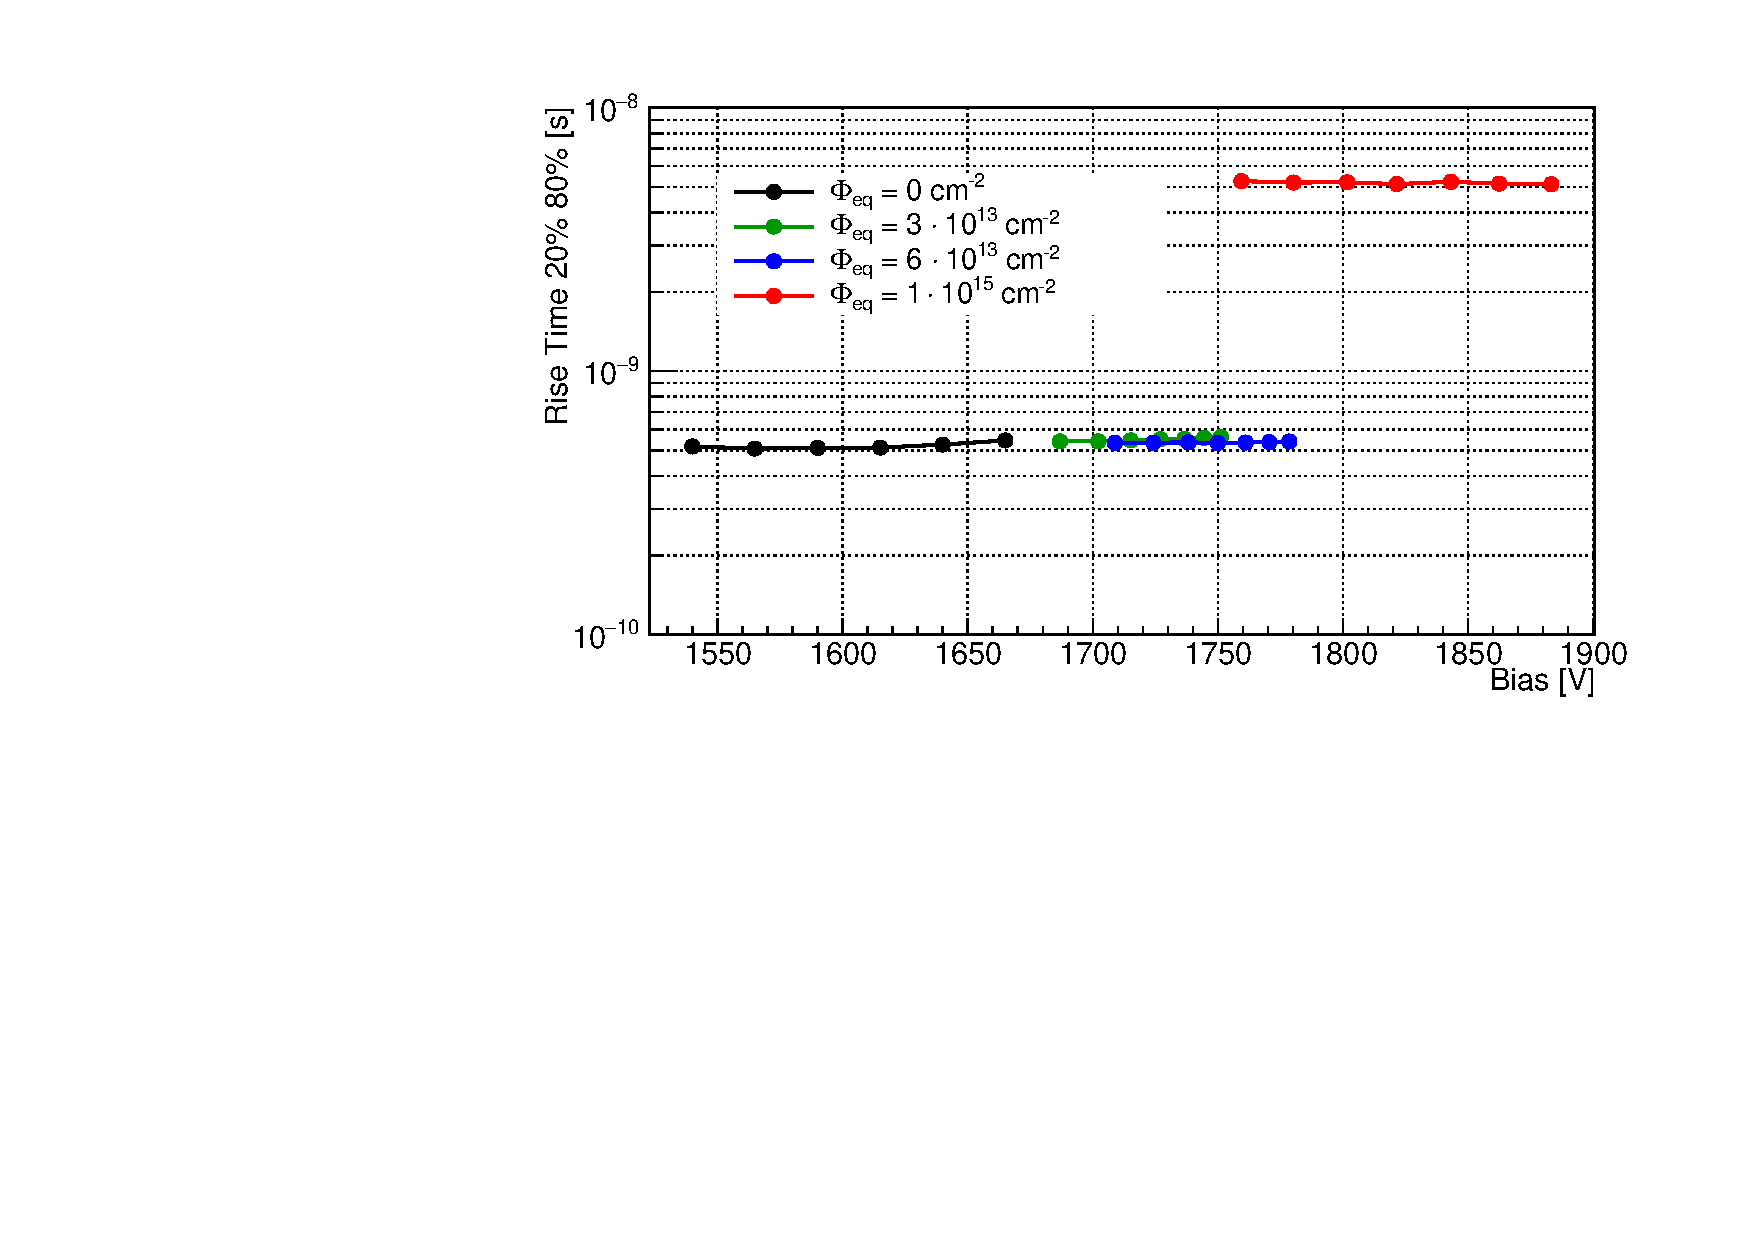
\includegraphics[width = 0.6 \textwidth]{riseTime2x2APDs}
  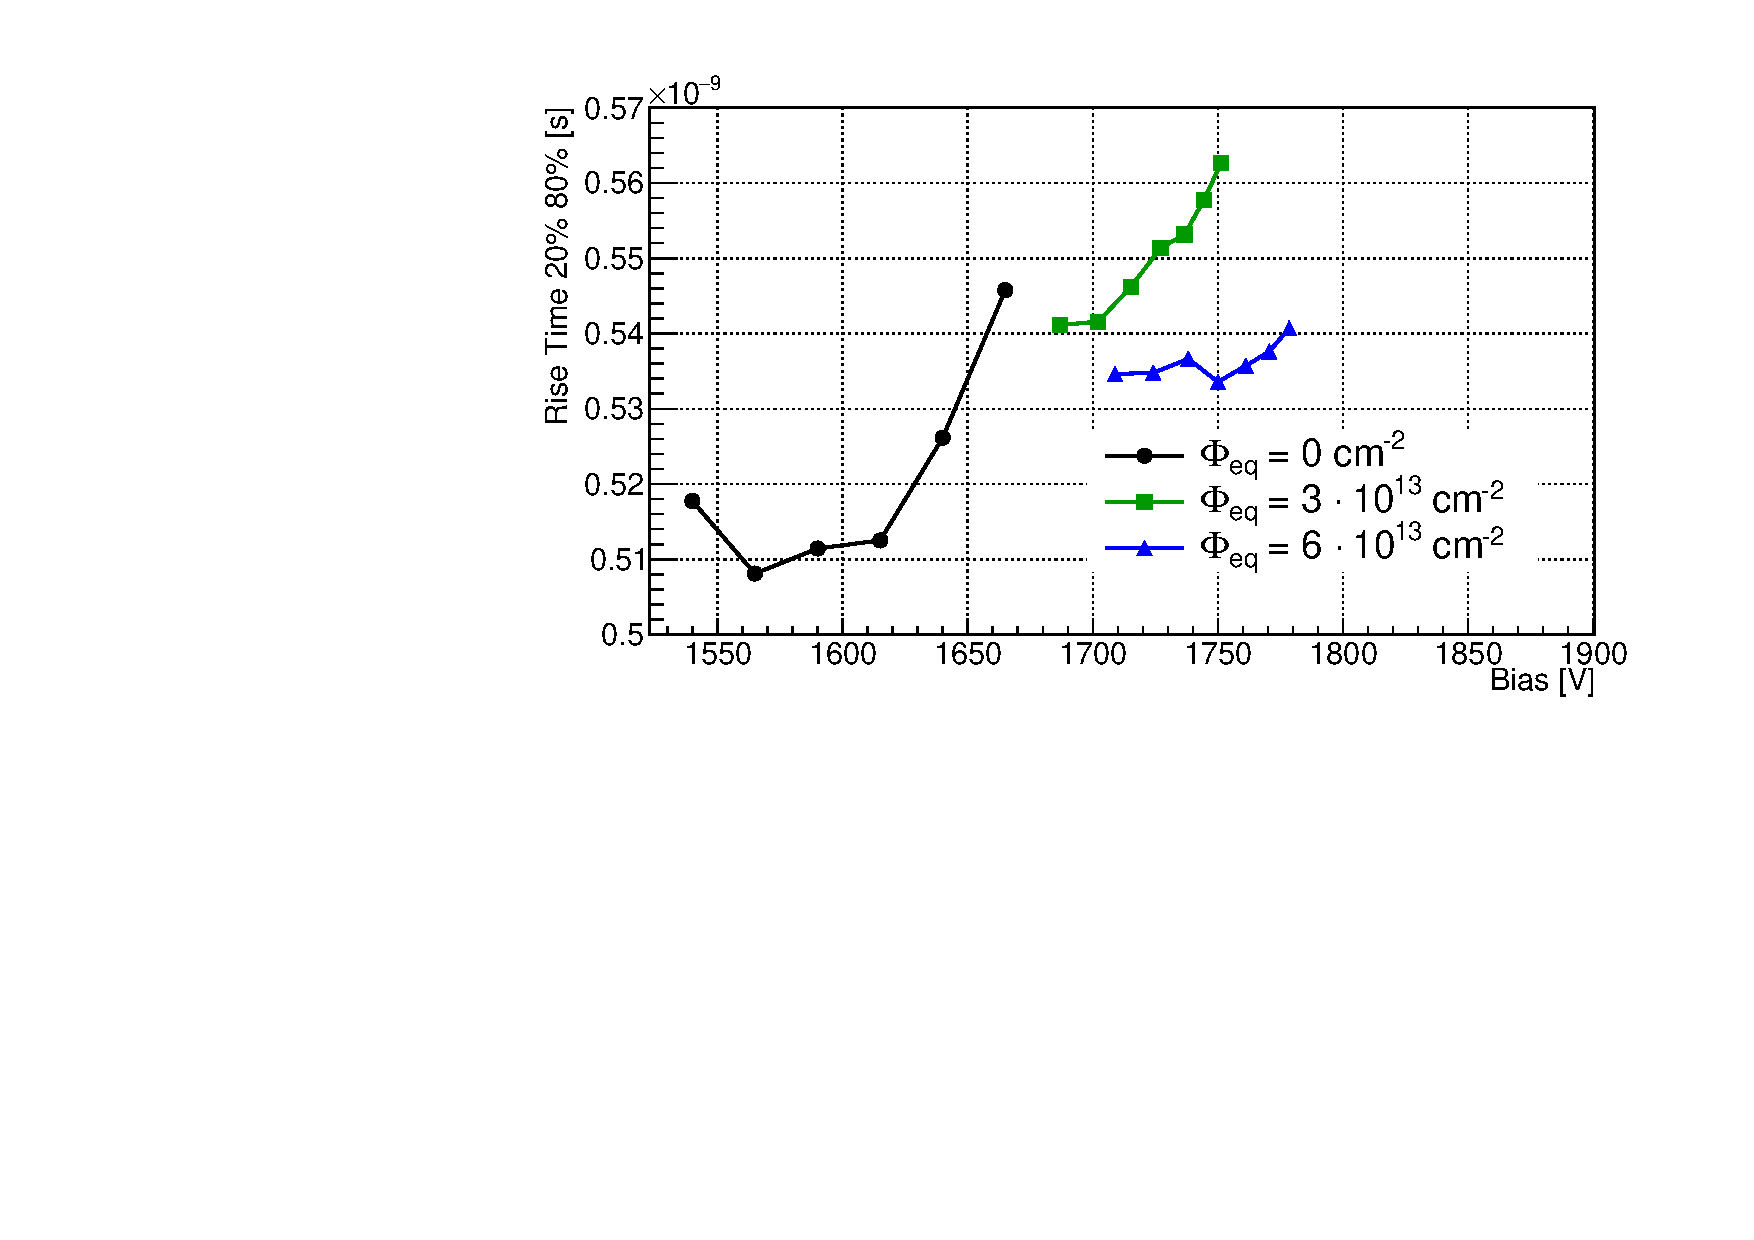
\includegraphics[width = 0.6 \textwidth]{riseTime2x2APDsNo1e15}
  \caption{20\%-to-80\% rise time of the $2 \times 2$~mm$^2$ APDs signal as a function of bias voltage and fluence measured at $-20^\circ$C. The laser intensity corresponds to 0.8\,MIPs. An amplification of 40\,dB was used.}
  \label{fig:riseTime2x2}
\end{figure}

The time resolution of the sensors was determined using the two pulses acquired in each waveform.
The waveforms are divided in two parts of 50\,ns each.
The pulses are analysed independently.
The time difference between the pulses is calculated using a constant fraction discriminator (CFD) algorithm.
This algorithm was chosen since it allows to study the effect of different thresholds applied to the pulses with relative ease, without having to account for the pulse amplitude.
The thresholds applied to the pulses were optimised for each measurement condition, choosing the combination that resulted in the best time resolution.
The time resolution is defined as the standard deviation of the distribution of the time difference ($\Delta t$) between the pulses.
The crossing time of the thresholds was determined using a linear interpolation between two points of the waveform.
Since the difference in the amplitude of the pulses measured in the same waveform was less than 5\%, the time jitter of the sensor and readout electronics for a single pulse (or single pulse time resolution) can be calculated by dividing the two pulses time resolution by $\sqrt{2}$.
The single pulse time resolution of the detectors is shown in figure\,\ref{fig:timeRes2x2} as a function of bias and fluence.
The jitter of the sensor irradiated to $\Phi_{eq} = 10^{15}$\,cm$^{-2}$ lies between 508 and 553\,ps.
These values are not shown in the figure for clarity.
The other sensors show a trend of decreasing jitter as a function of bias voltage.
The behaviour is however not monotonous.

%1e15 -> time res 508-553 ps
\begin{figure}
  \centering
  %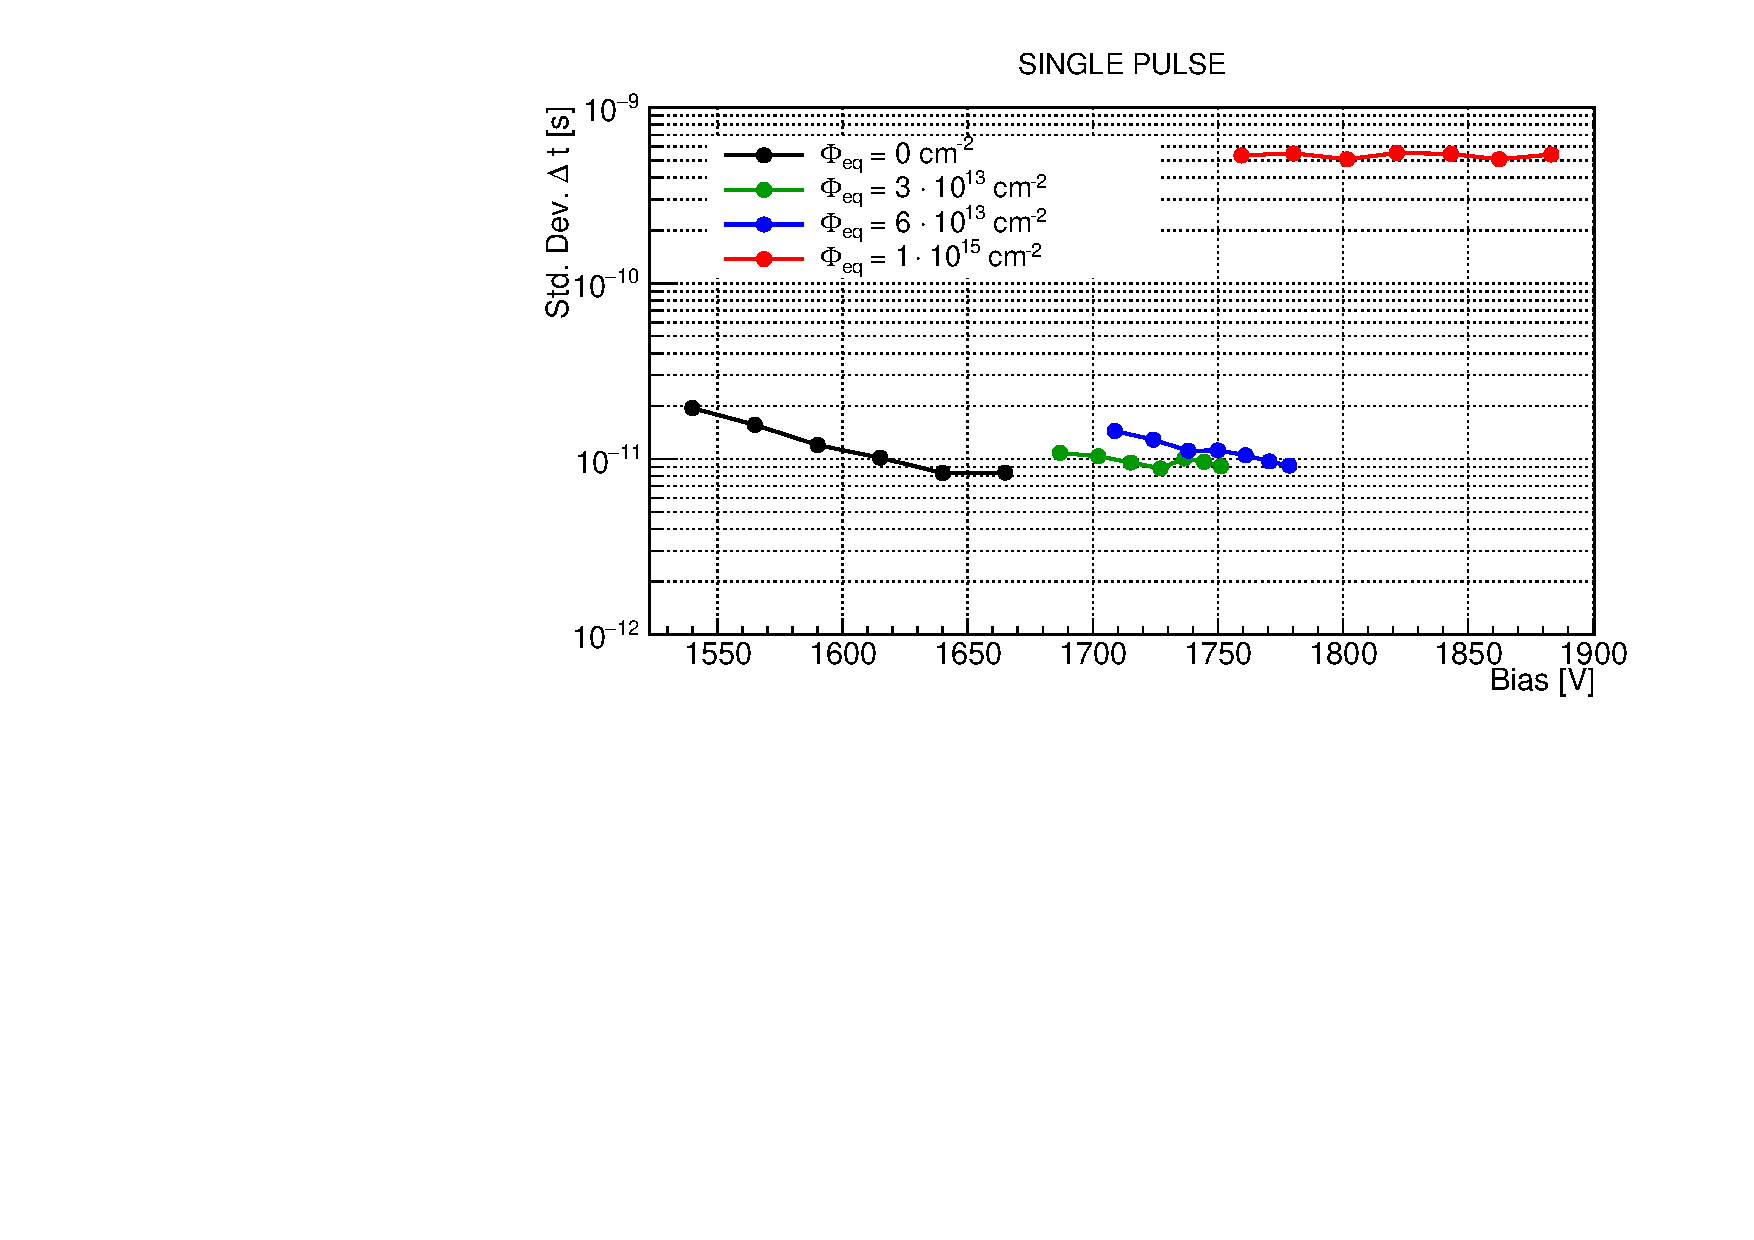
\includegraphics[width = 0.6 \textwidth]{timeRes2x2APDs}
  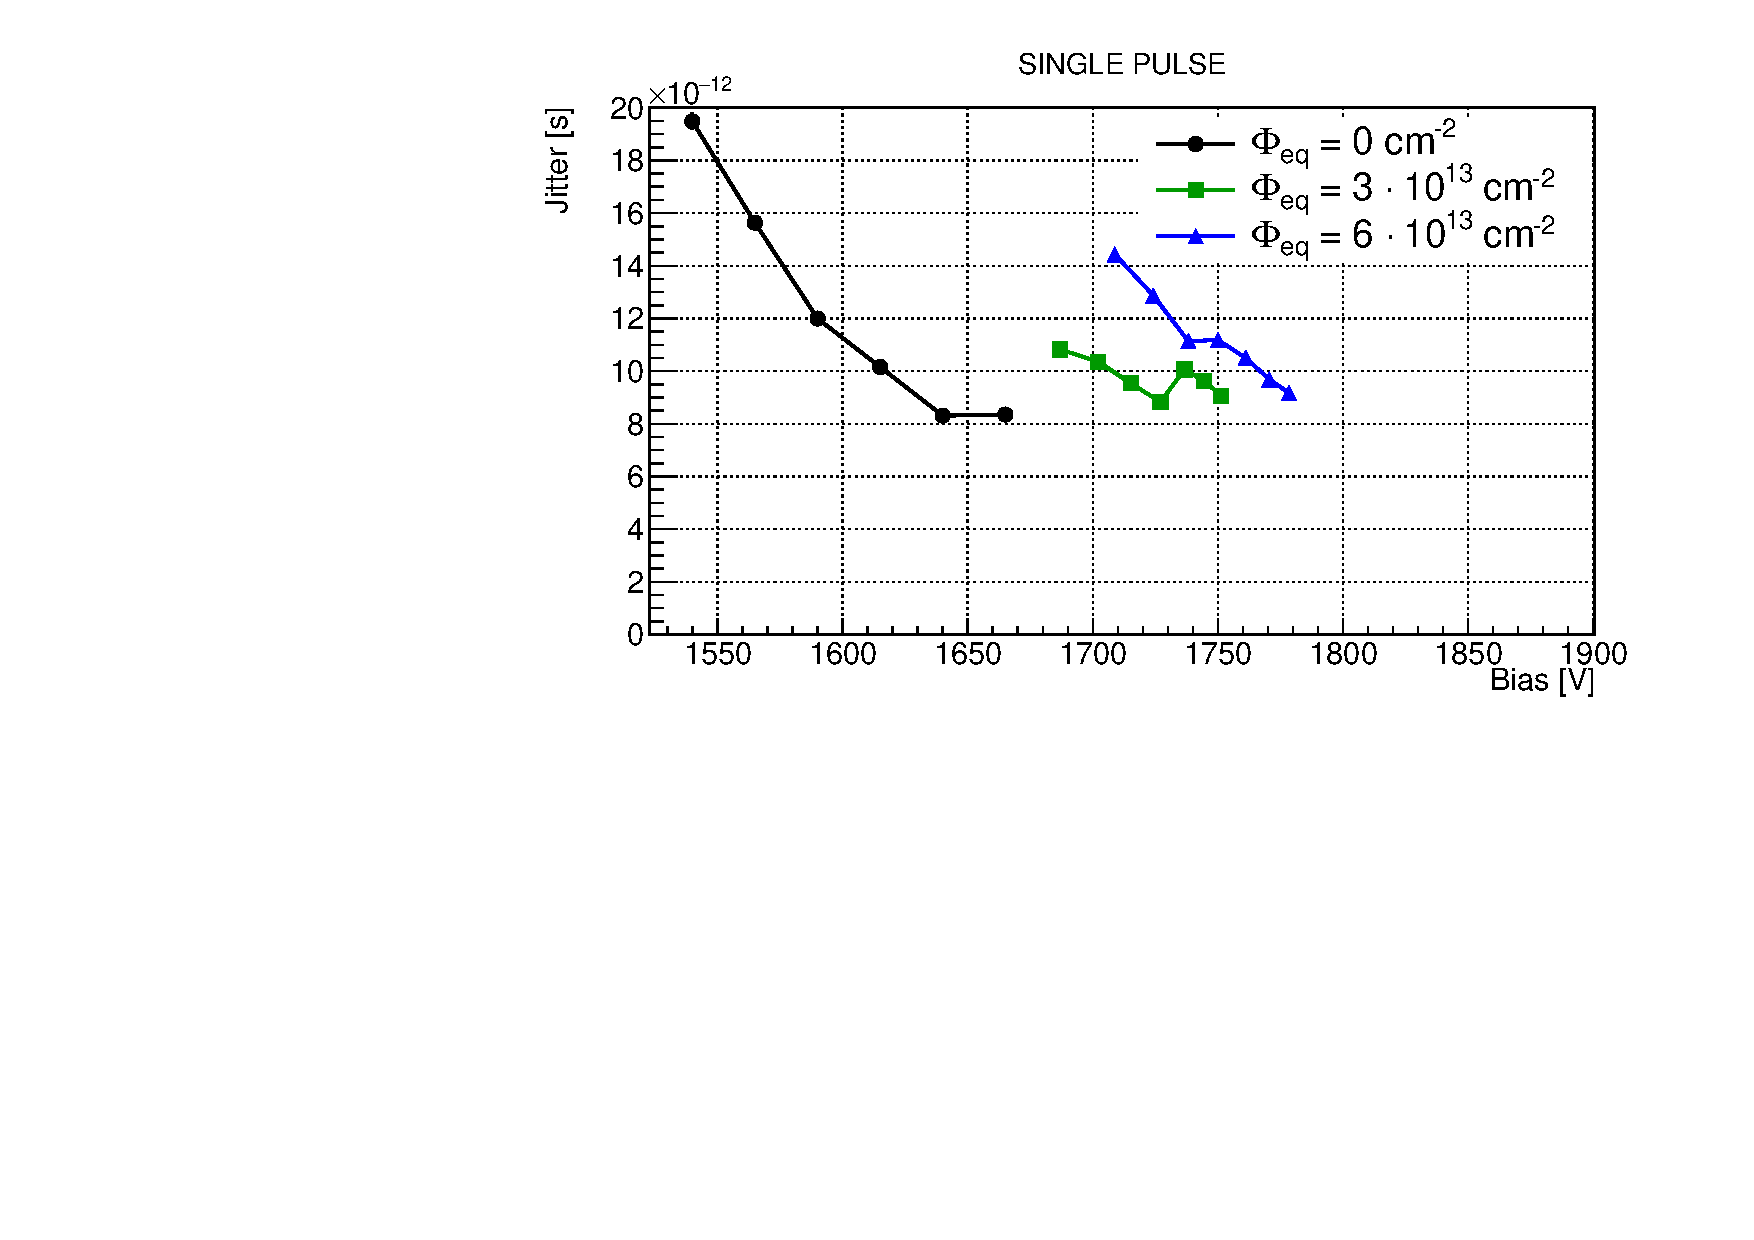
\includegraphics[width = 0.6 \textwidth]{timeRes2x2APDsNo1e15}
  \caption{Single pulse time resolution of the $2 \times 2$~mm$^2$ APDs as a function of bias voltage and fluence measured at $-20^\circ$C. The laser intensity corresponds to 0.8\,MIPs. An amplification of 40\,dB was used.}
  \label{fig:timeRes2x2}
\end{figure}

The jitter is found to scale approximately as 1/SNR.
Figure\,\ref{fig:timeRes2x2_snr} shows the jitter as a function of SNR.
The dashed line represents a 1/SNR behaviour.

\begin{figure}
  \centering
  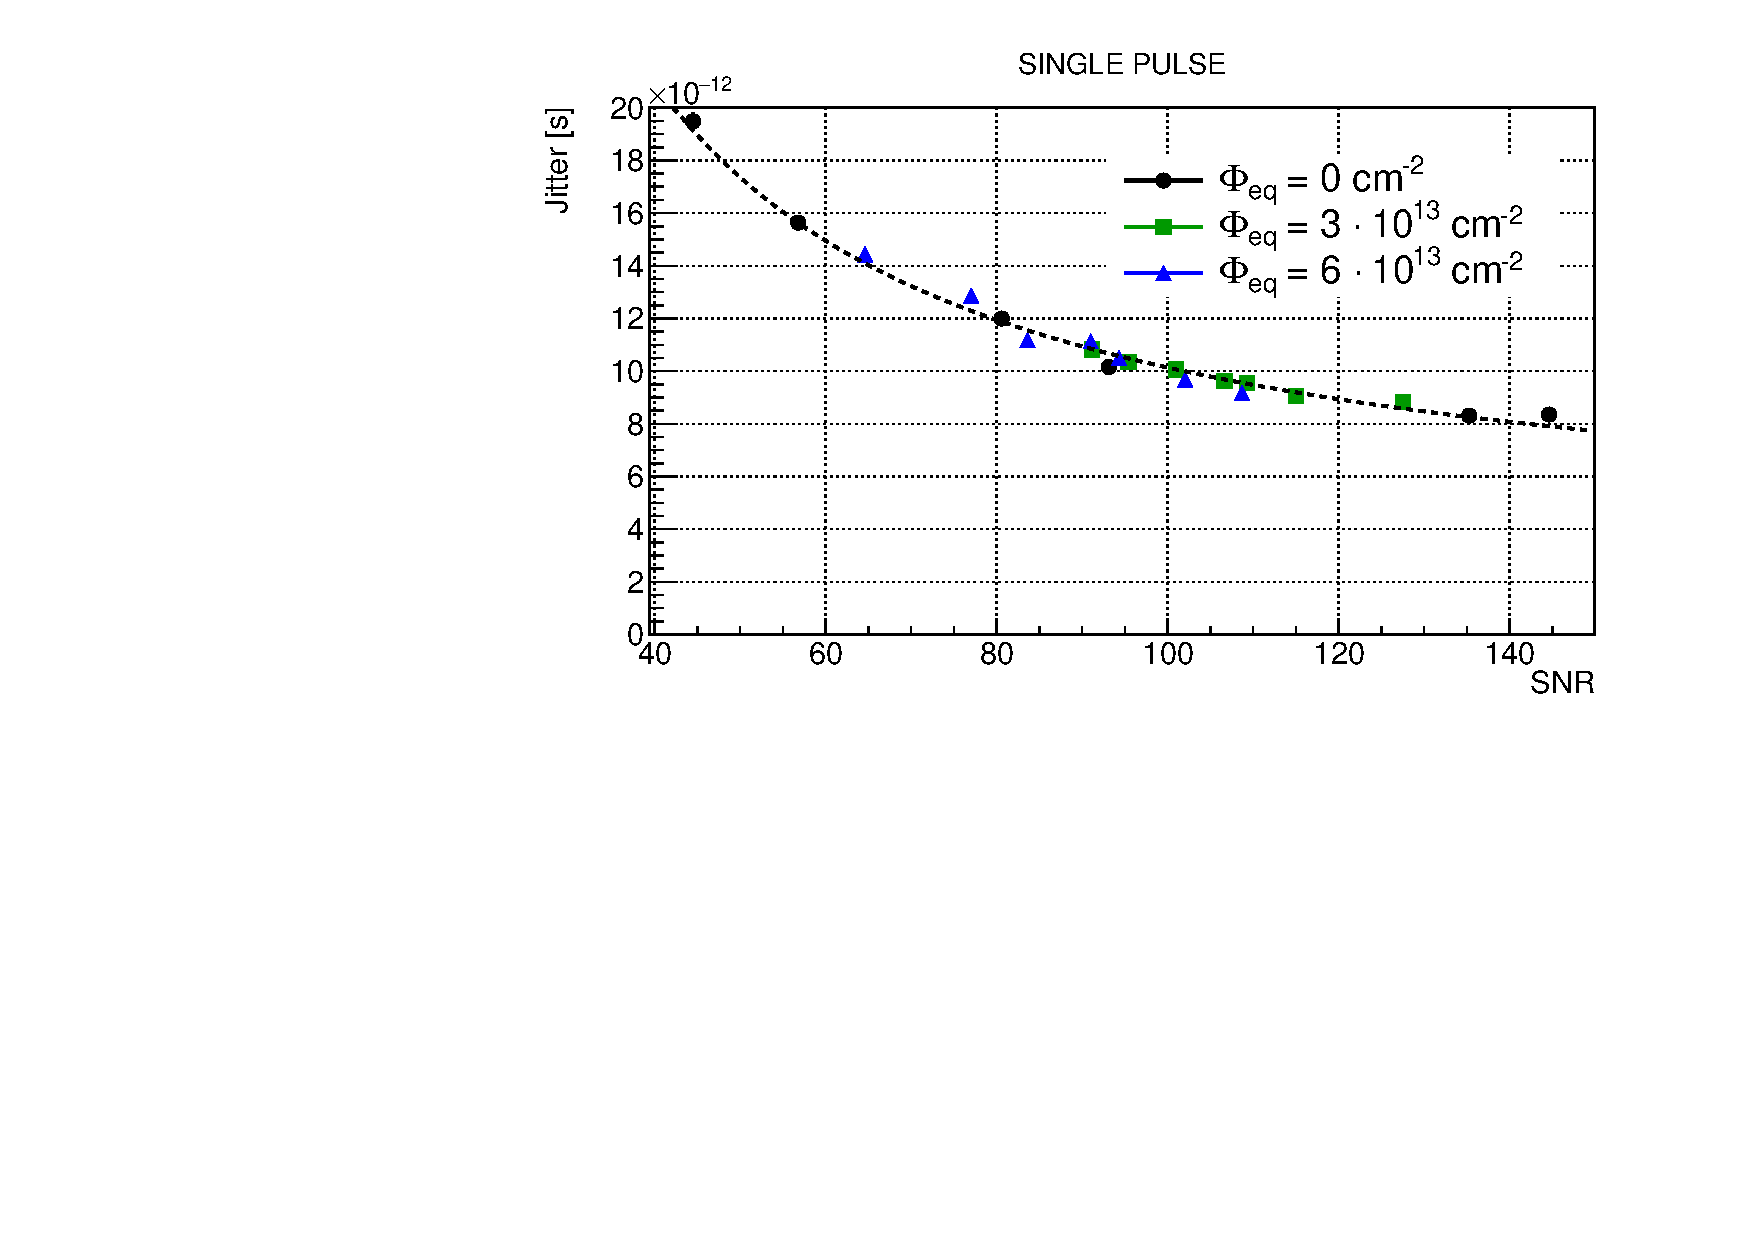
\includegraphics[width = 0.6 \textwidth]{timeRes2x2APDsNo1e15_SNR}
  \caption{Single pulse time resolution of the $2 \times 2$~mm$^2$ APDs as a function of signal to noise ratio and fluence measured at $-20^\circ$C. The laser intensity corresponds to 0.8\,MIPs. An amplification of 40\,dB was used.}
  \label{fig:timeRes2x2_snr}
\end{figure}

The jitter of the sensors is not degraded by the neutron-induced radiation damage corresponding to a fluence of at least $\Phi_{eq} = 6 \cdot 10^{13}$\,cm$^{-2}$.
This result is expected to hold for timing measurements of charged particles.
The overall resolution is however expected to worsen due to the fluctuations of the amount of charge deposited per unit length along the particle path.
These fluctuations, also known as {\em Landau noise}\,\cite{cartiglia2017}, can influence the leading edge of the sensor's signal and therefore worsen the time resolution.

\section{Uniformity Study of $8 \times 8$~mm$^2$ APDs using an Infrared Laser}
\label{sec:unif8x8laser}

The uniformity of response of the $8 \times 8$~mm$^2$ APDs was studied using an infrared laser.
The amplitude and integrated signal are shown in figure\,\ref{fig:8x8unif_noMetal} as a function of the position were the laser illuminated the detector.
The sensor was mounted with the n-side facing the PCB, and the laser shone on the p-side.
The sensor was contacted using opaque conductive paint.
The point of contact on the p-side can be seen at the coordinate (4.5, 6)\,mm.
Since the absorption length of the light used in the measurements is greater than the sensor thickness, several features of the surface below the sensor can be seen in the figure.
The square mesa structure and the conductive paint used to glue the detector to the PCB used for the measurements can be seen as areas of increased amplitude and signal integral due to their reflection of the light toward the sensor.
The PCB has a hole below the detector centre, that results in decreased values of amplitude and signal integral.
Since the signal amplitude is affected by both the deposited charge in the detector and the detector properties, the amplitude was normalised using the integrated signal in order to mitigate the former effect.
The ratio between the amplitude and the integrated signal is shown in figure\,\ref{fig:8x8unif_noMetal}.
The effects of the surface below the sensor are reduced and a dependency of the ratio between amplitude and charge on the distance between the laser spot and the point where the signal is collected from the sensor can be seen.
The amplitude of the signal decreases with increasing distance from the electrical contact.
This effect is attributed to the non-negligible resistivity of the conductive layers applied to the detector.
The dependency of the signal amplitude on the detector position can result in a worsened time resolution.

\begin{figure}
  \centering
  \subfloat[Amplitude]{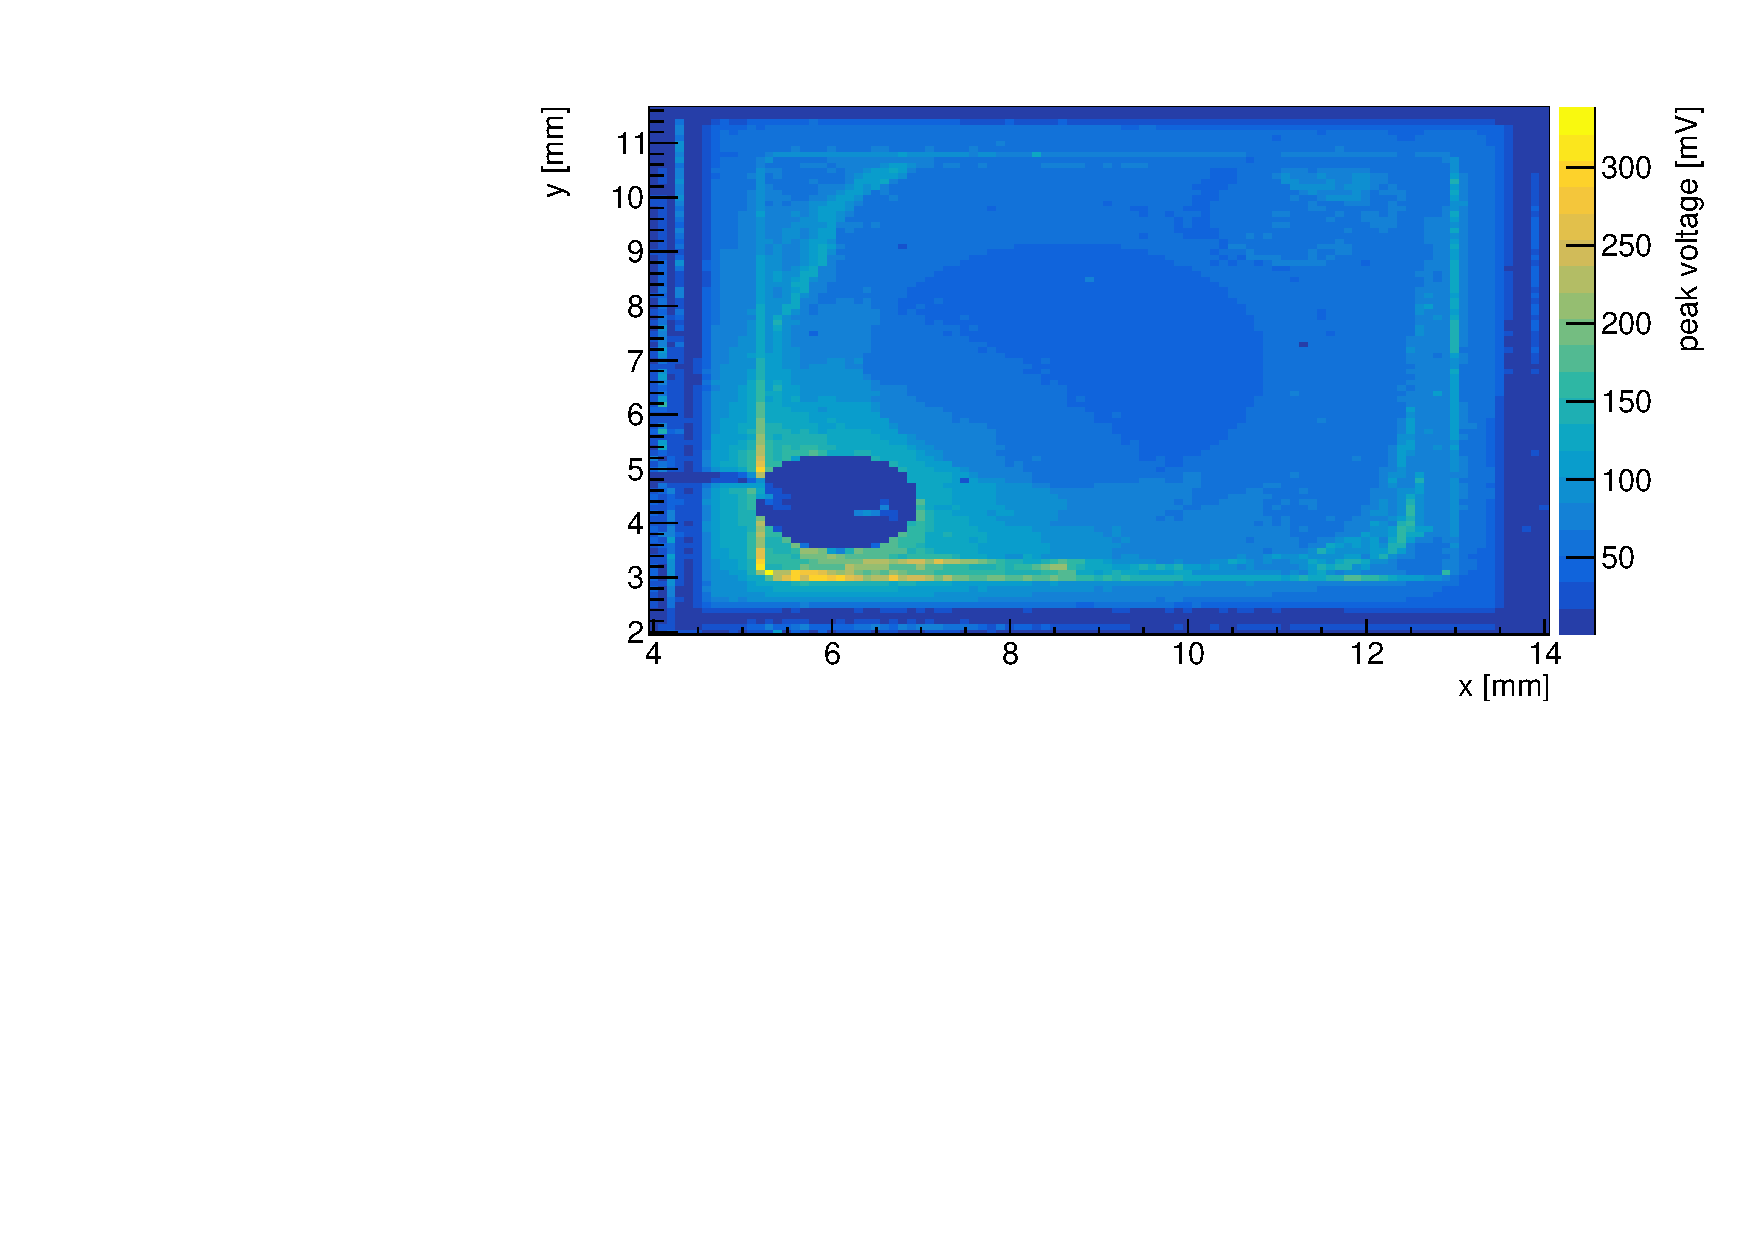
\includegraphics[width = 0.45 \textwidth]{peakMap8x8fine}}\hfill
  \subfloat[Integrated signal]{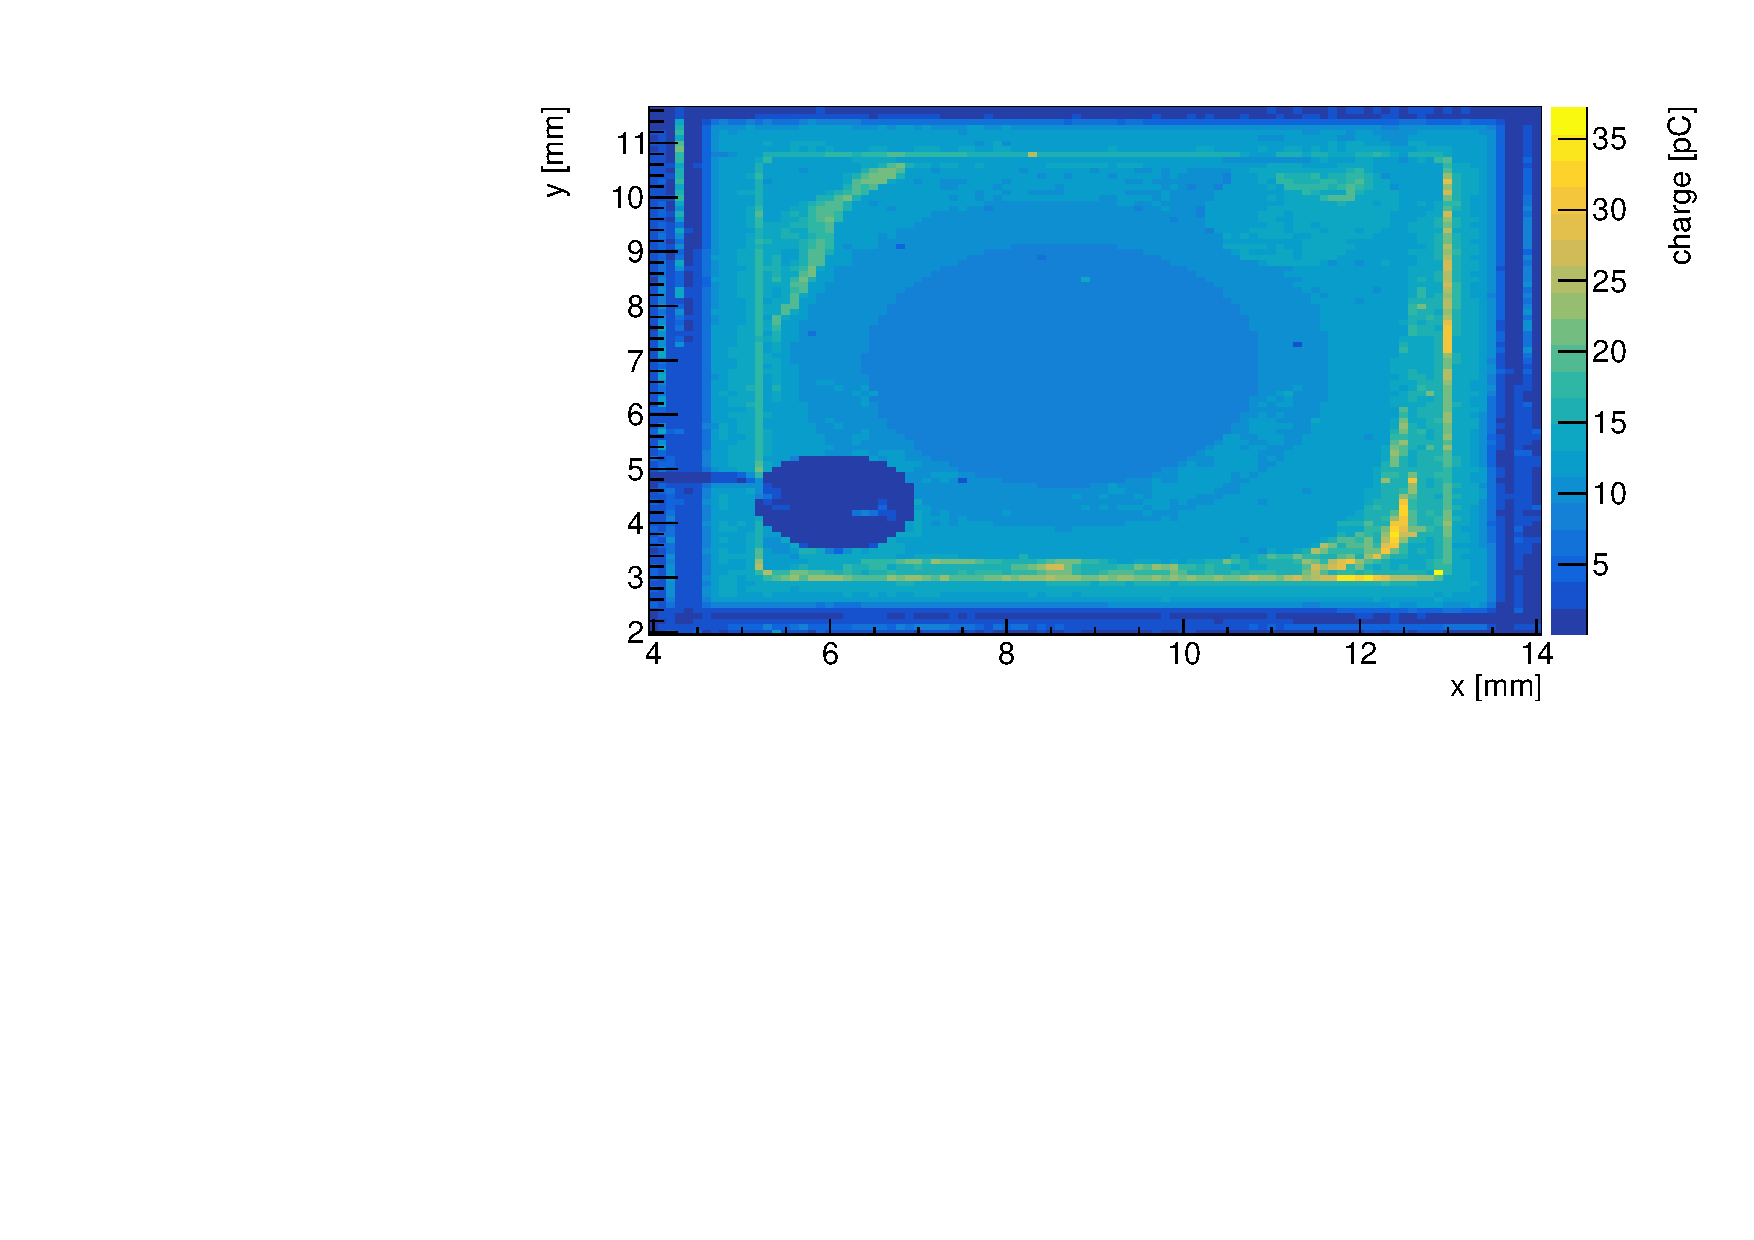
\includegraphics[width = 0.45 \textwidth]{chargeMap8x8fine}}\\
  \subfloat[Ratio]{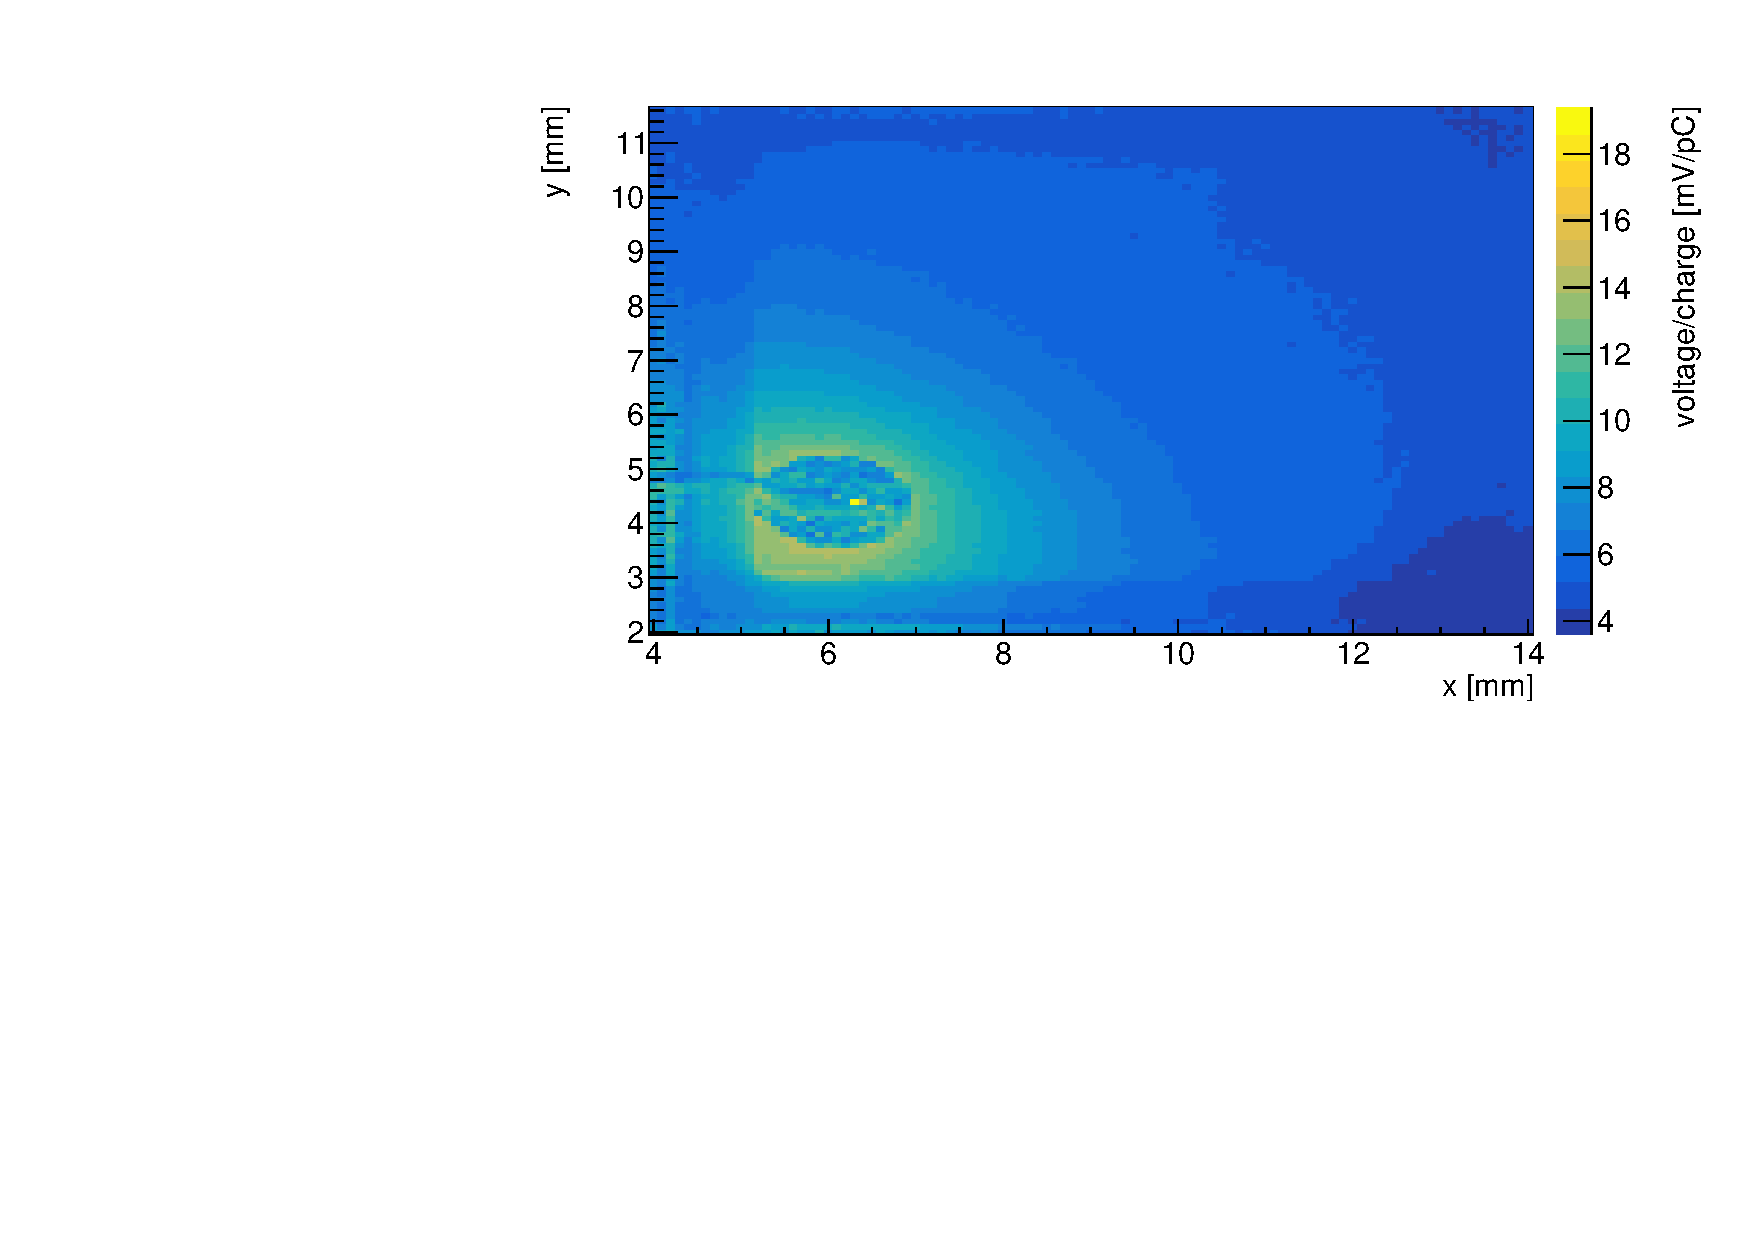
\includegraphics[width = 0.45 \textwidth]{ratioPeakChargeMap8x8fine}}\hfill
  \subfloat[Ratio vs distance]{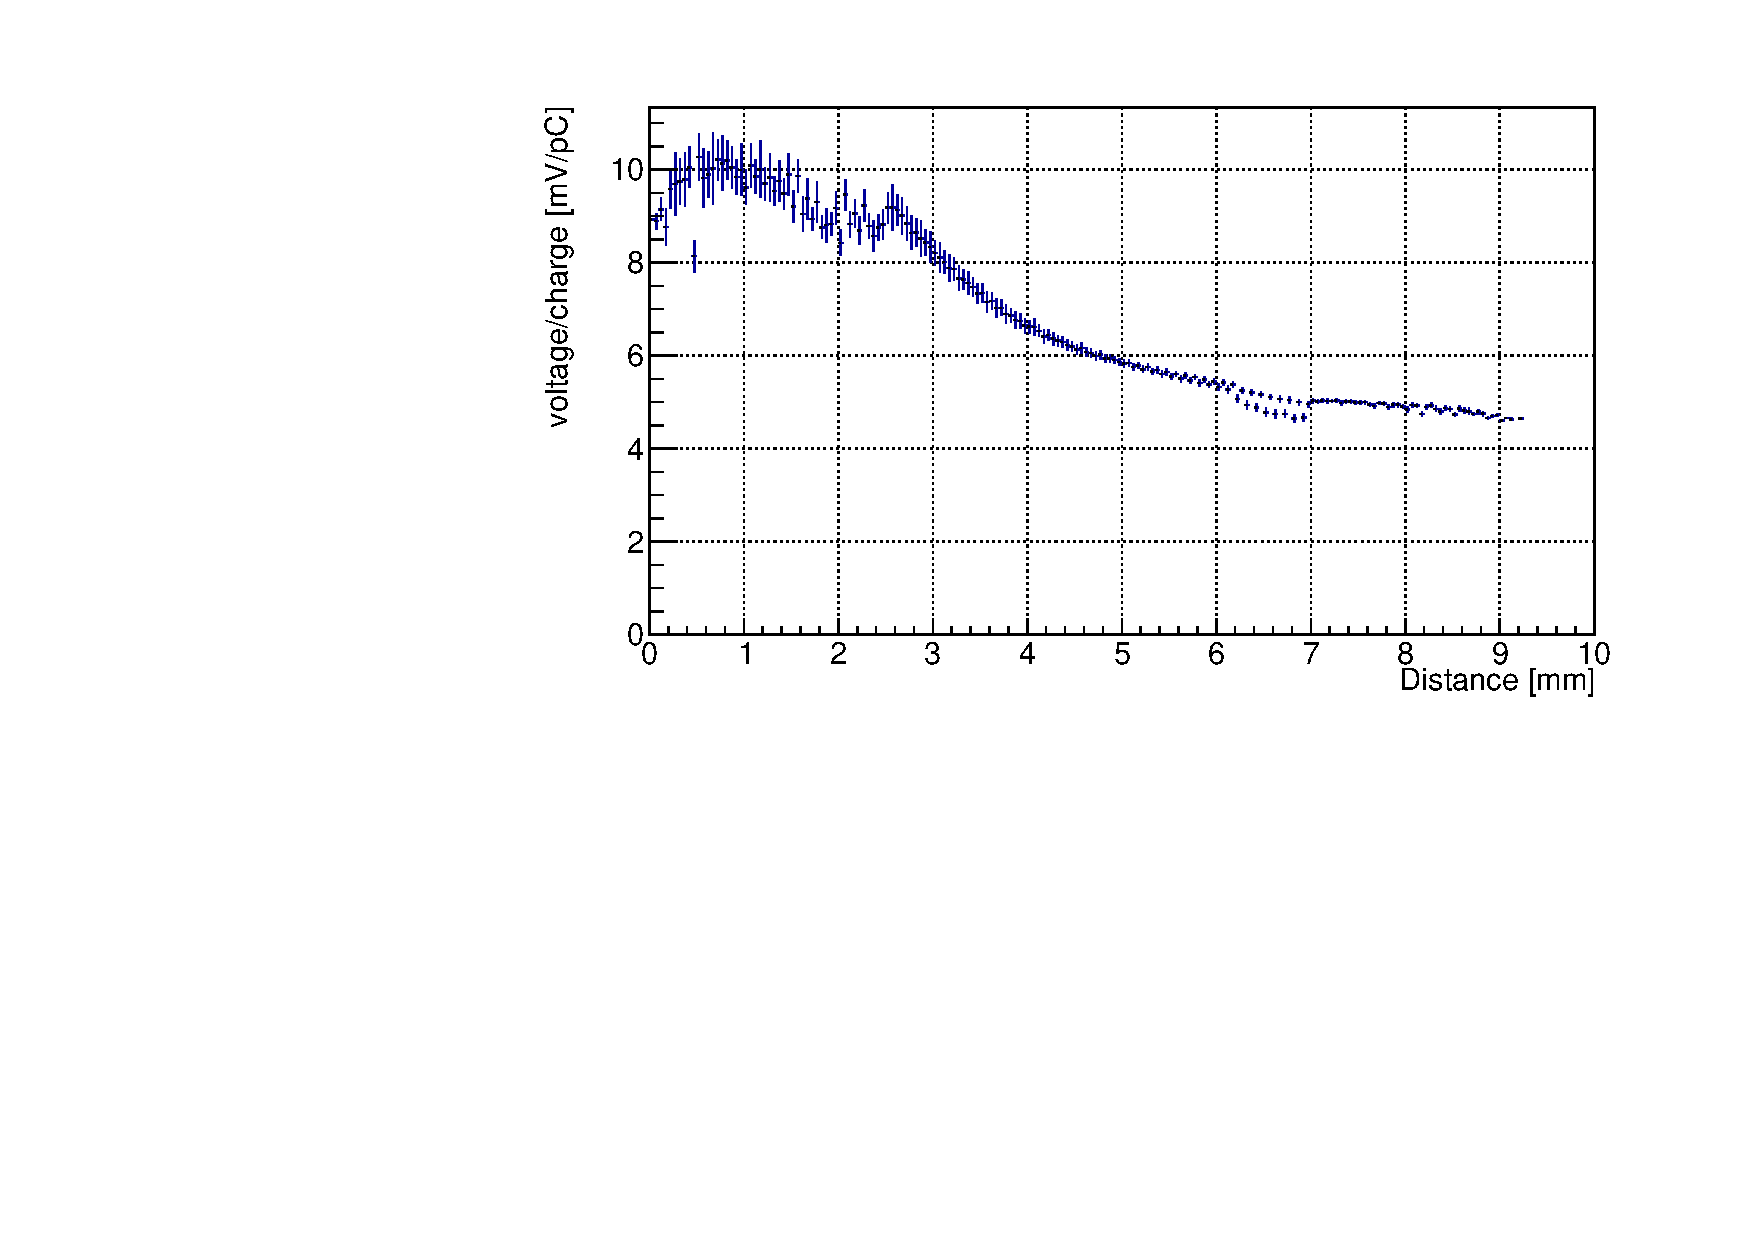
\includegraphics[width = 0.45 \textwidth]{ratioPeakChargeDistance}}\\
  \caption{Signal amplitude {\bf (a)}, integral {\bf (b)}, and ratio between amplitude and integral {\bf (c)} of a $8 \times 8$~mm$^2$ APD as a function of position. {\bf (d)} Ratio between amplitude and integral as a function of distance from the electrical contact of the sensor. The sensor was biased at 1700\,V, at a temperature of $-20^\circ$C. The laser intensity corresponds to 15 MIPs. An amplification of 10\,dB was used.}
  \label{fig:8x8unif_noMetal}
\end{figure}

The two approaches taken to reduce this source of non-uniformity are described in section\,\ref{sec:samples}.
%% The results obtained with the AC-coupled mesh readout are shown in section\,\ref{sec:tb8x8}.
The DC-coupled metallisation resulted in a difference in the ratio between amplitude and charge of less than 2\% over a distance of 7\,mm between the points illuminated by the laser.
No dependency on the distance between illumination and electrical contact was observed.
This measurement was performed on a sensor biased to 1800\,V at a temperature of $20^\circ$C.
The metallisation was performed at the clean room facility of CMi-EPFL\,\cite{cmi}.
The structure consists of an aluminium grid on the n-side and a continuous aluminium layer with an opening at the detector centre on the p-side of the detector.
This configuration allows the illumination of the detector centre without reflections.

\section{Timing Performance of $8 \times 8$~mm$^2$ APDs using an Infrared Laser}
\label{sec:timing8x8laser}

The time resolution of the metallised $8 \times 8$~mm$^2$ APDs with DC-coupled readout was studied using the same setup and procedure used for the characterisation of the irradiated $2 \times 2$~mm$^2$ APDs in section\,\ref{sec:irrad2x2}.
A light intensity corresponding to 0.8\,MIPs and an amplification of 40\,dB were used.
The light was shone in the centre of the detector.
The signal amplitude and noise are shown in figure\,\ref{fig:ampli8x8metal} and\,\ref{fig:noise8x8metal}, respectively.
The signal amplitude is smaller than the one of the $2 \times 2$~mm$^2$ devices shown in section\,\ref{sec:irrad2x2}.
This can be a consequence of a lower gain of the device under test or the bigger capacitance of the device.
The noise is also smaller than the one of the $2 \times 2$~mm$^2$ devices.
Both signal amplitude and noise increase as a function of bias voltage.
The signal to noise ratio is lower than the one of the non-irradiated $2 \times 2$~mm$^2$ APD presented in section\,\ref{sec:irrad2x2}, ranging from 18 to 62.

\begin{figure}
  \centering
  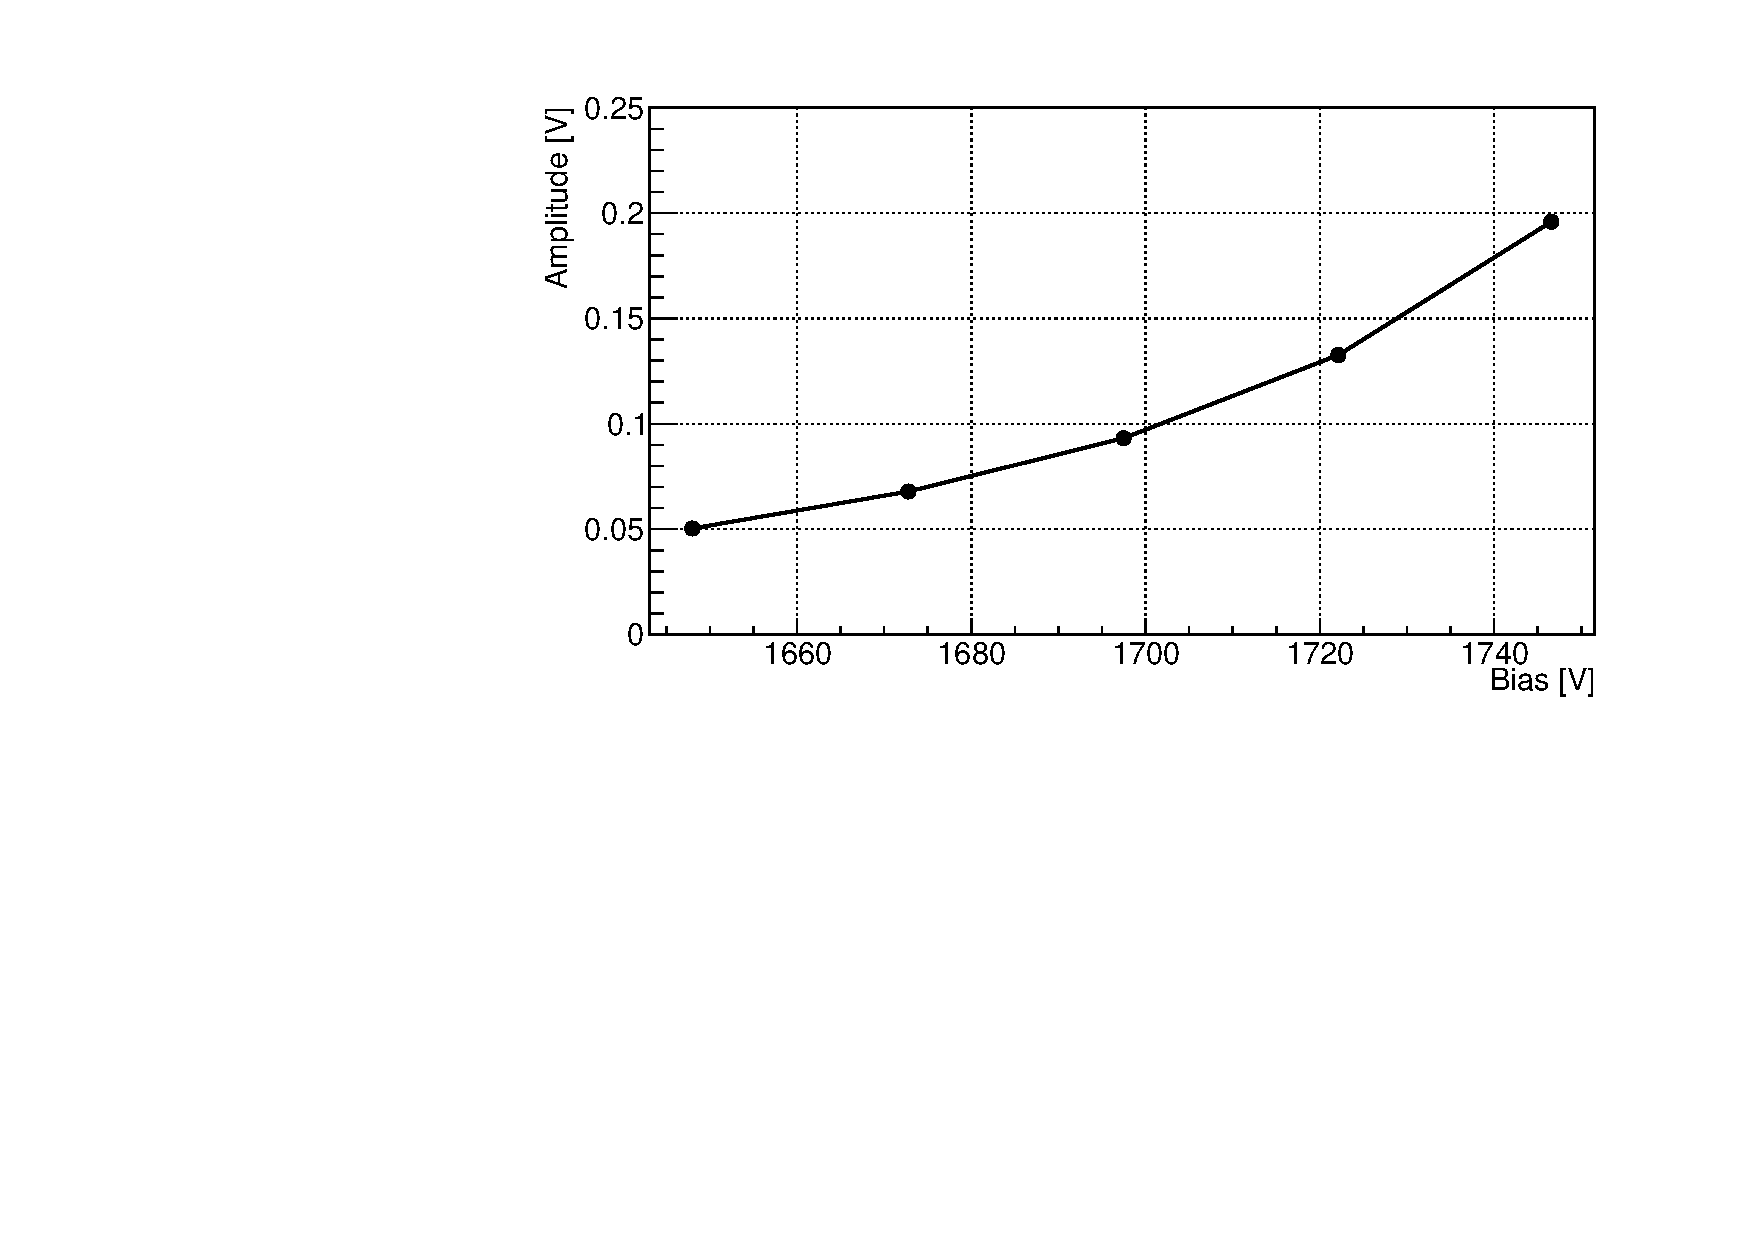
\includegraphics[width = 0.6 \textwidth]{ampli8x8metal}
  \caption{Average amplitude of the metallised $8 \times 8$~mm$^2$ APD signal as a function of bias voltage measured at $20^\circ$C. The laser intensity corresponds to 0.8\,MIPs. An amplification of 40\,dB was used.}
  \label{fig:ampli8x8metal}
\end{figure}

\begin{figure}
  \centering
  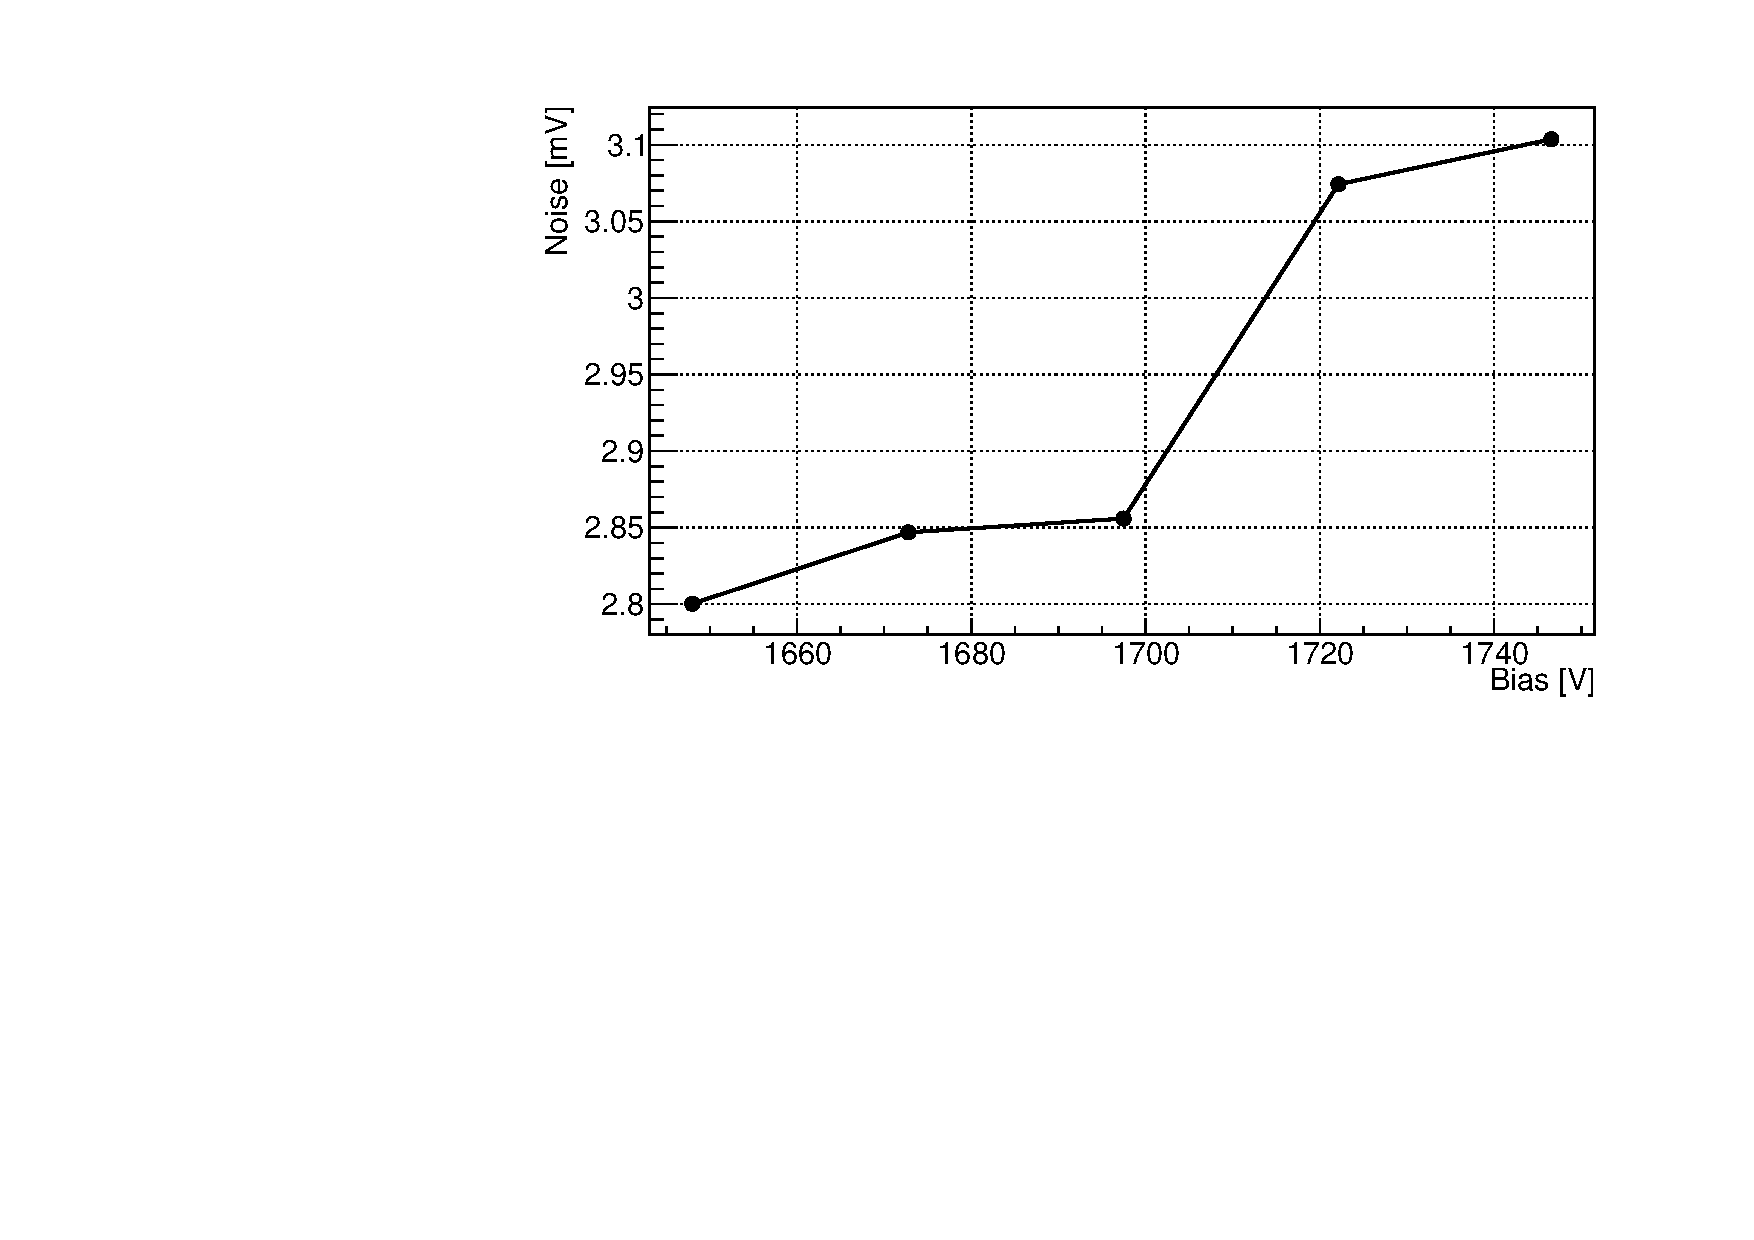
\includegraphics[width = 0.6 \textwidth]{noise8x8metal}
  \caption{$8 \times 8$~mm$^2$ APD's noise as a function of bias voltage measured at $20^\circ$C. An amplification of 40\,dB was used.}
  \label{fig:noise8x8metal}
\end{figure}

The 20\%-to-80\% rise time of the signal is shown in figure\,\ref{fig:riseTime8x8metal}.
The values are bigger than the ones of the $2 \times 2$~mm$^2$ devices.
This is a consequence of the bigger sensor capacitance.

\begin{figure}
  \centering
  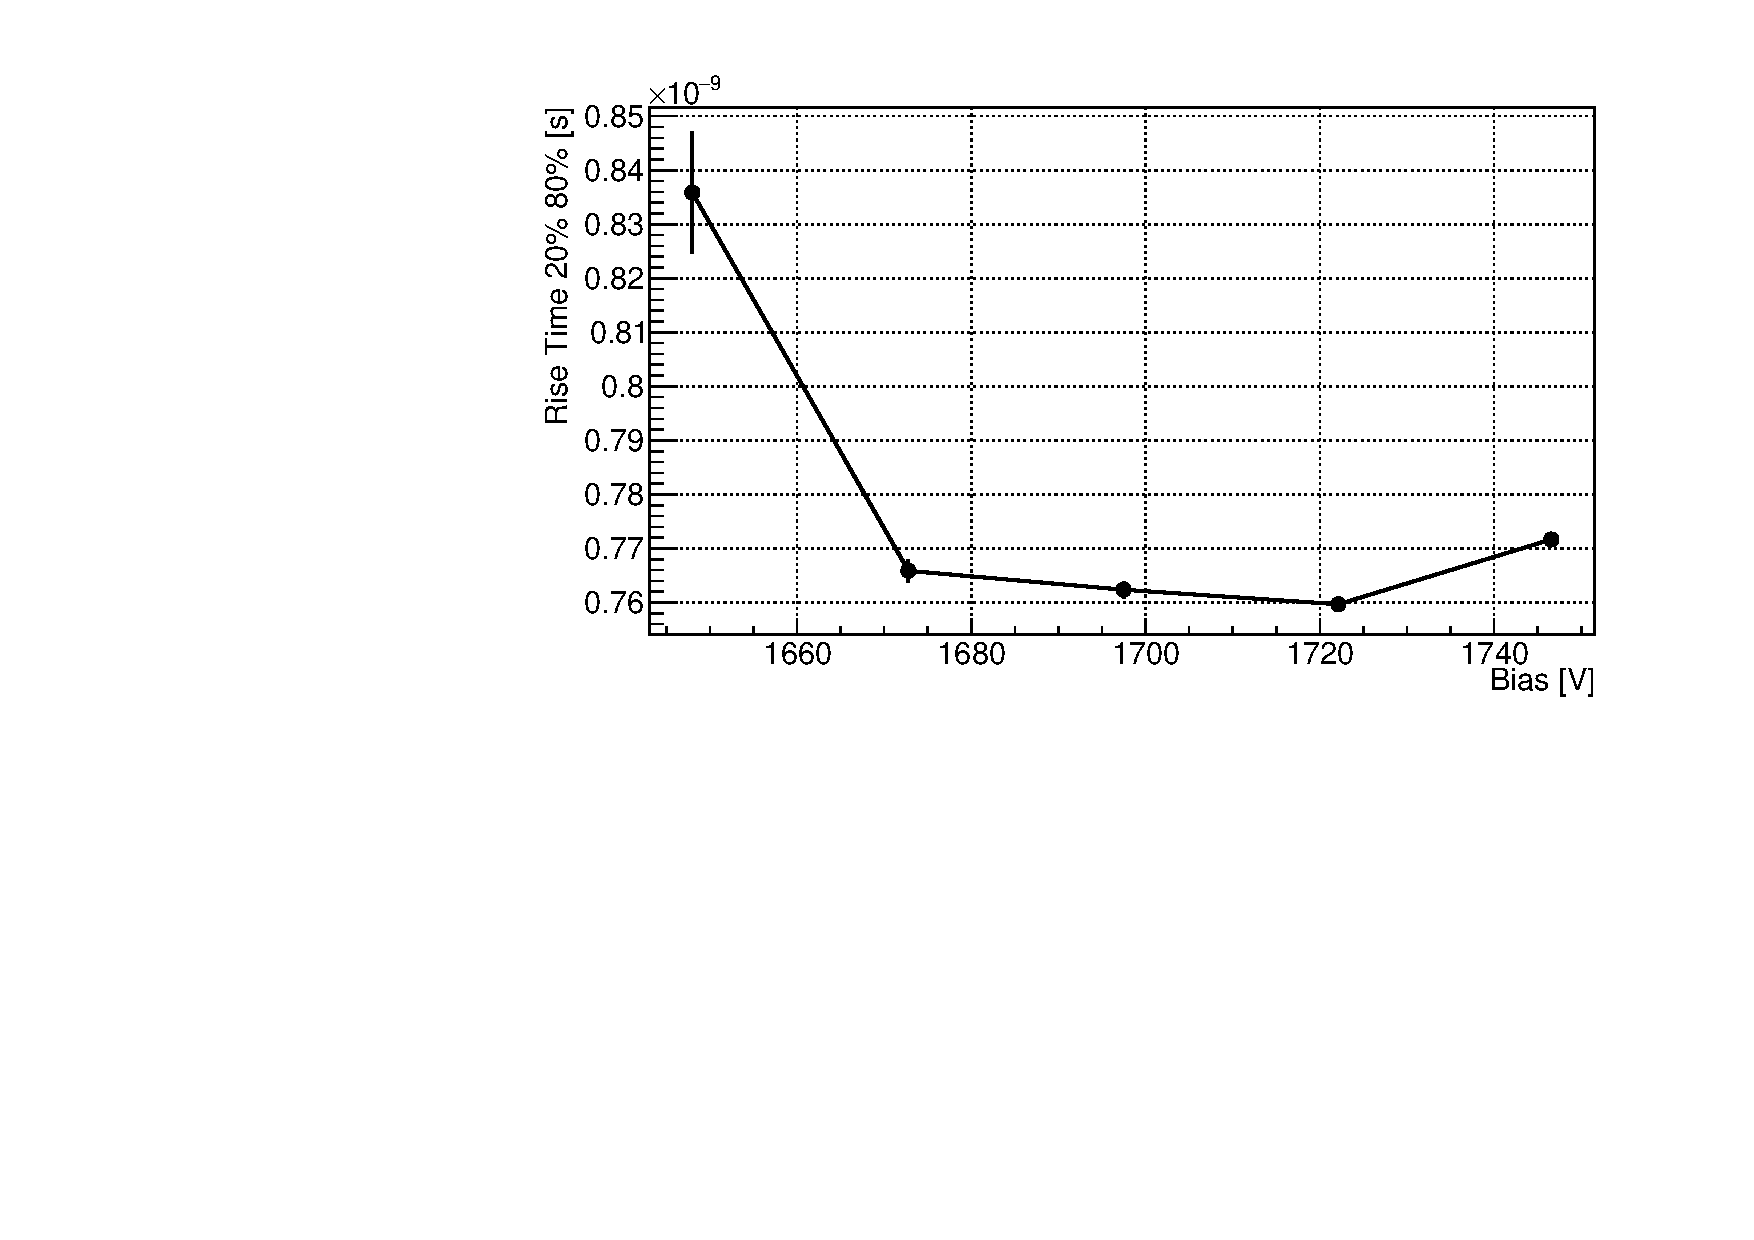
\includegraphics[width = 0.6 \textwidth]{riseTime8x8metal}
  \caption{20\%-to-80\% rise time of the metallised $8 \times 8$~mm$^2$ APD signal as a function of bias voltage measured at $20^\circ$C. The laser intensity corresponds to 0.8\,MIPs. An amplification of 40\,dB was used.}
  \label{fig:riseTime8x8metal}
\end{figure}

The jitter was calculated with the same procedure presented in section\,\ref{sec:irrad2x2}.
The jitter decreases with increasing bias voltage and is found to scale with a 1/SNR behaviour.

\begin{figure}
  \centering
  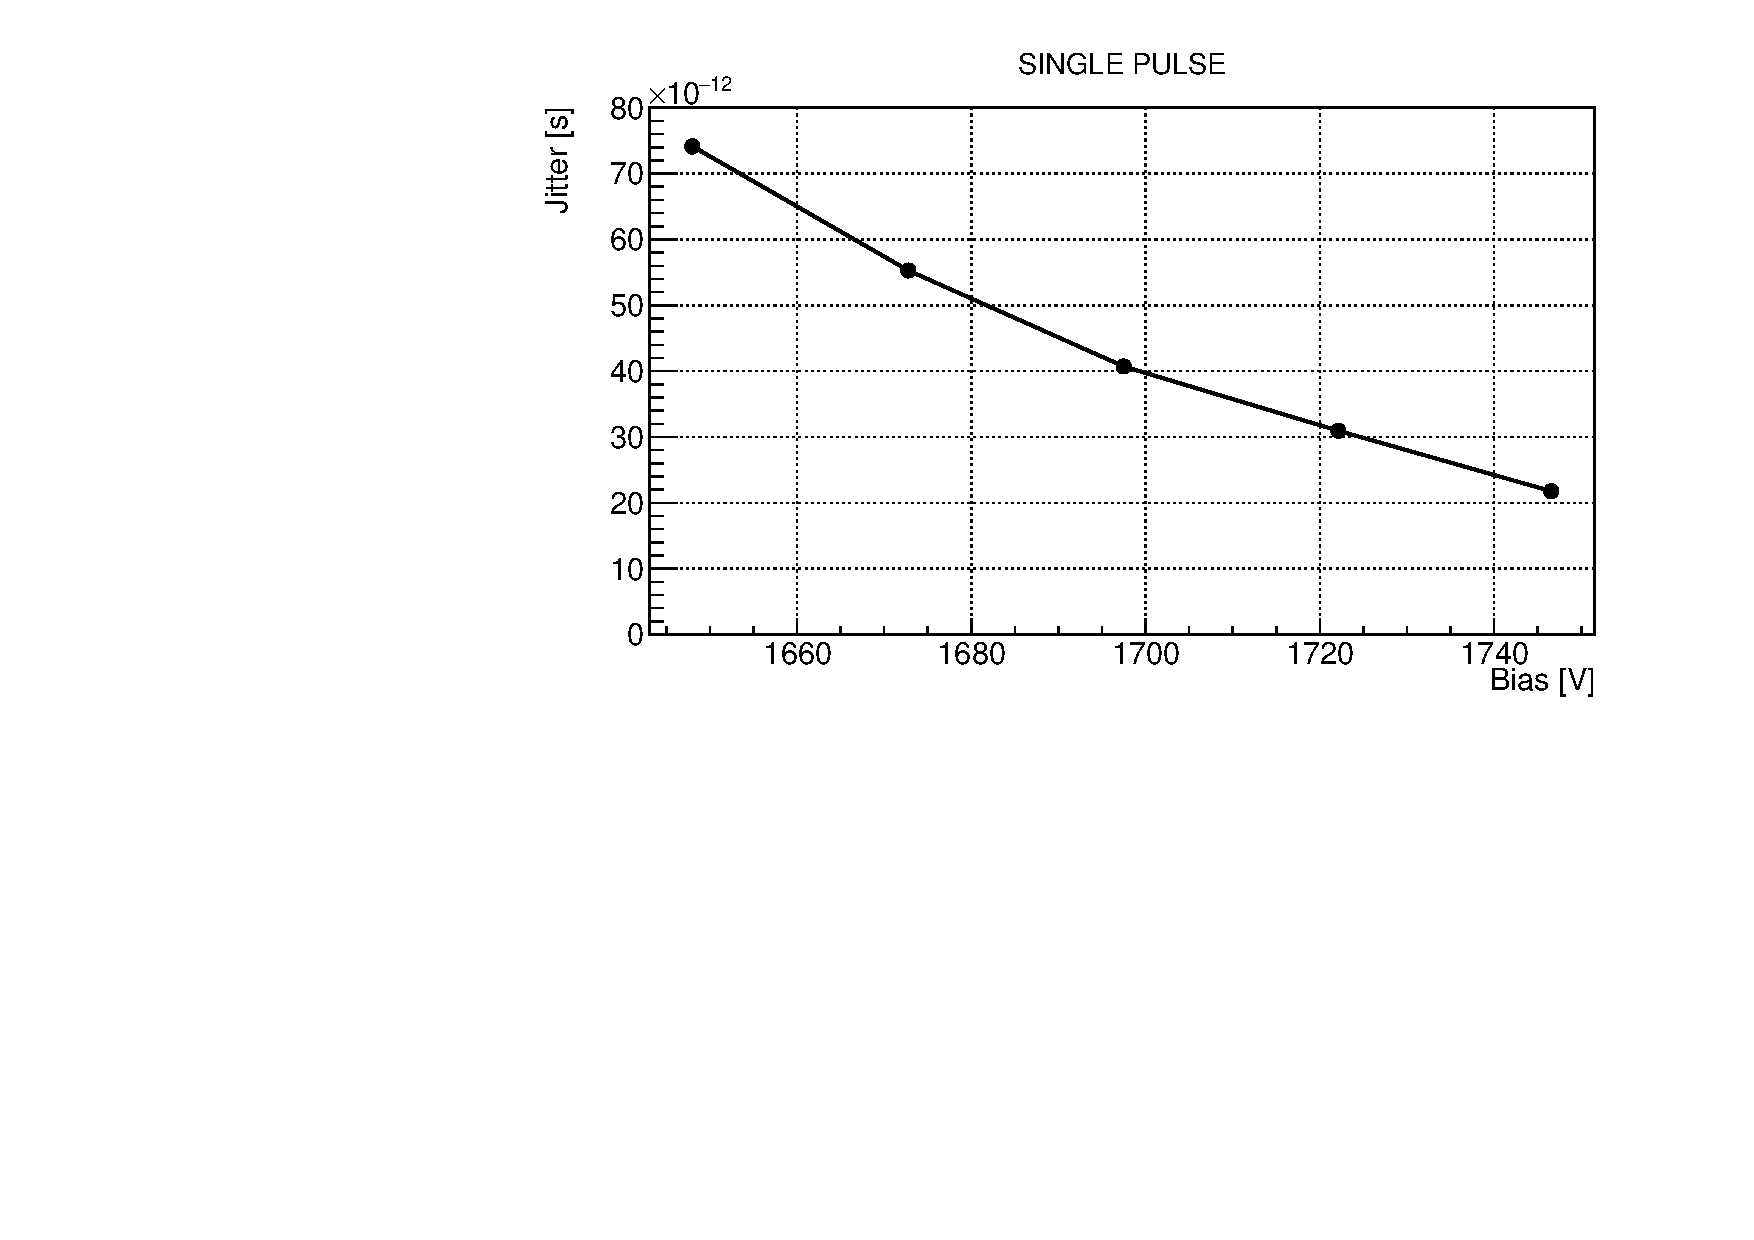
\includegraphics[width = 0.6 \textwidth]{timeRes8x8metal}
  \caption{Single pulse time resolution of the metallised $8 \times 8$~mm$^2$ APDs as a function of bias voltage measured at $20^\circ$C. The laser intensity corresponds to 0.8\,MIPs. An amplification of 40\,dB was used.}
  \label{fig:timeRes8x8metal}
\end{figure}

The metallised $8 \times 8$~mm$^2$ APDs often did not allow for a stable operation when biased above 1700\,V.
The source of the instability is under investigation.
This instability influenced the choice of values of bias voltage used in this section.

\section{Beam Tests of $8 \times 8$~mm$^2$ APDs with AC-coupled Readout}
\label{sec:tb8x8}

Several mesh readout $8 \times 8$~mm$^2$ APDs were characterized in terms of their uniformity of response using a 150 GeV muon beam in the H4 beam line at the CERN SPS \textcolor{red}{ref?}.
For the measurements described below a fast transimpedence amplifier with roughly 10 ohm effective input impedance was used
\textcolor{red}{(ref. suggestion from Mitch)}.
The bandwidth of the amplifier was 1 GHz.
The measurements were carried out within the infrastructure of PICOSEC\,\cite{bortfeld2018}.
In particular, the PICOSEC setup provided particle tracking with a resolution of 40 $\mu$m and a time reference based on a Hamamatsu MCP PMT\footnote{Micro Channel Plate Photomultiplier.} which detected charged particles by the Cerenkov light produced in the quartz entrance window providing a reference time jitter of $<10$ picoseconds\,\cite{sohl2018}.
\textcolor{red}{reference frame of the beam test? APD temperature?  Selection cuts?}

Using the above setup and a 2.5 GHz 20 GSa/s digital oscilloscope to record the waveforms the timing measurements of the mesh readout APDs were derived using a 20\% constant fraction algorithm to define the signal time of arrival.
To ensure the consistency of this timing measurement the dependence of the waveform characteristics and in particular the rise time dependence on the impact position of the muons was studied using the H4 beam data.
For this particular study a sample of $\approx$1000 events were recorded with the sensor operated at a bias of 1750~V resulting in a most probable amplitude (MIP peak) of 65~mV at the oscilloscope input.
The typical pulse rise time (measured at 20-80\% levels) was 630~ps with an RMS spread of $\approx$160~ps.
Figure\,\ref{fig:risetime8x8impact} shows the average risetime as a function of the impact position of the particles for both the $x$ and $y$ directions.
The rise time is essentially independent of the point of impact.
\begin{figure}
  \centering
  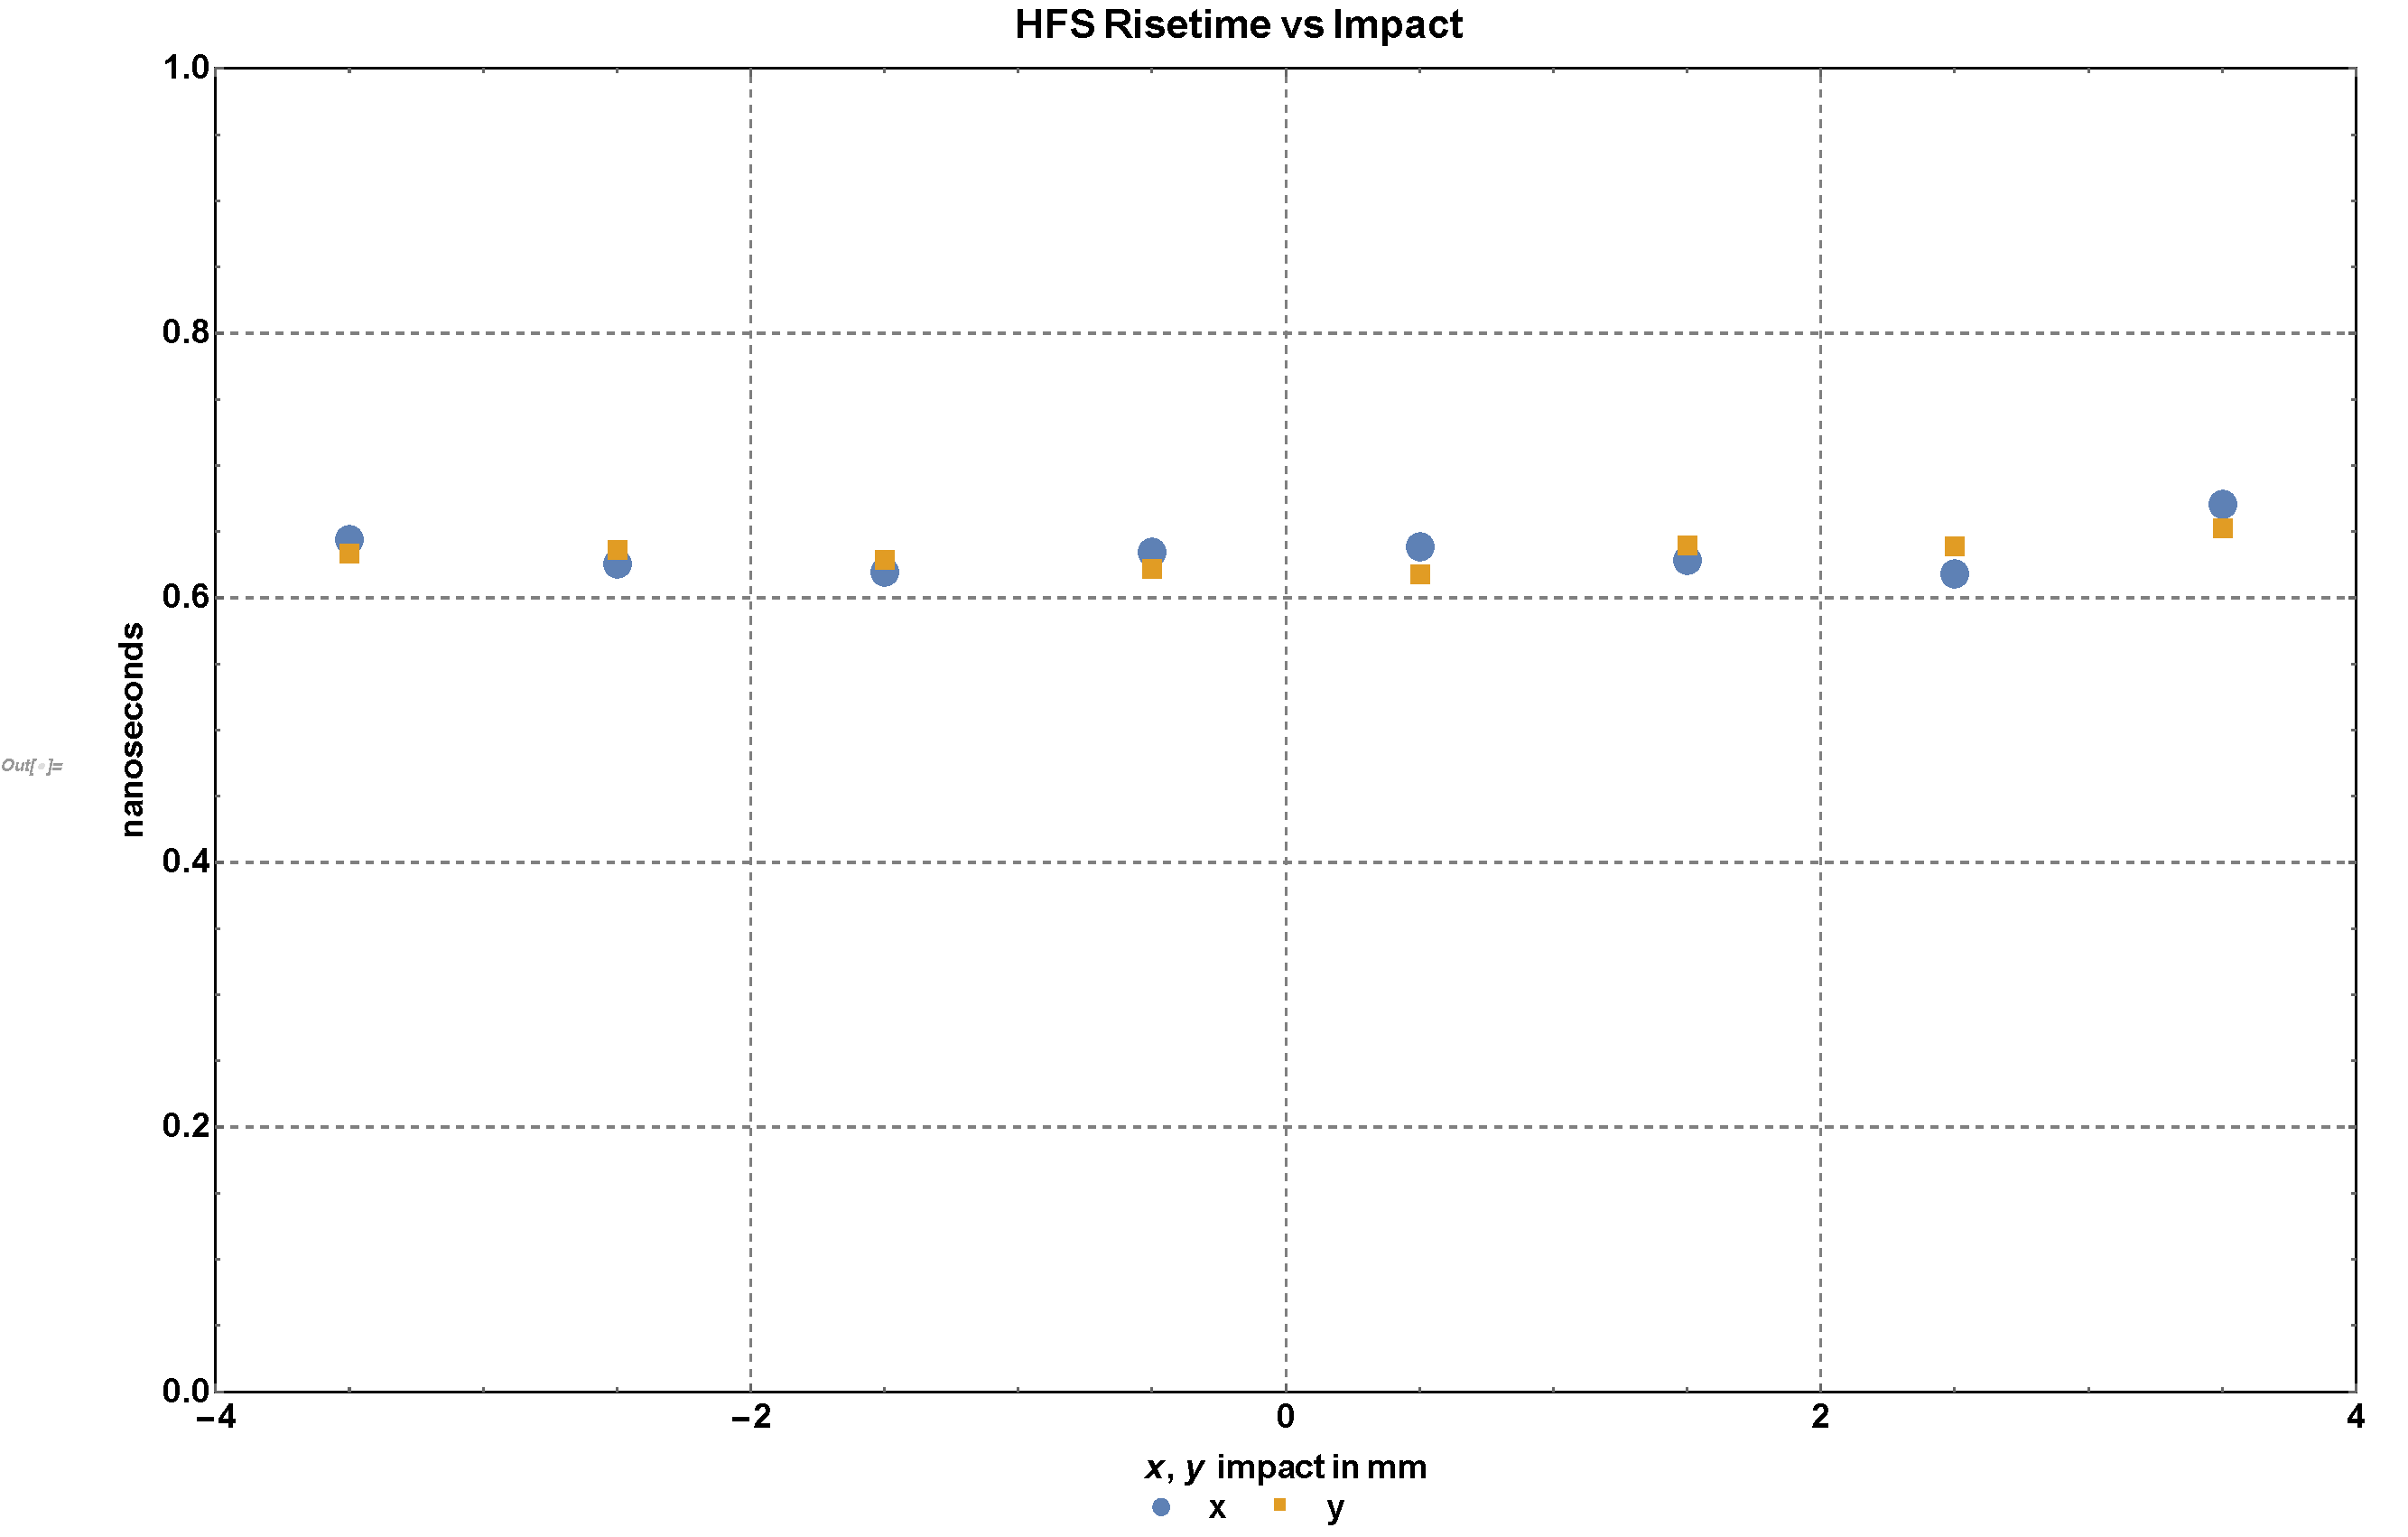
\includegraphics[width = 0.6 \textwidth]{risetime8x8vsImpact}
  \caption{Mean 20-to-80\% rise time as a function of impact position for a mesh readout APD. The measurement was performed using 150 GeV muons. The APD was operated at 1750 V, at a temperature of \textcolor{red}{...}$^\circ$C.}
  \label{fig:risetime8x8impact}
\end{figure}

Figure\,\ref{fig:toa8x8impact} shows the time of arrival of the particles as measured by the mesh readout APD as a function of impact position.
The MCP PMT is used to define the origin of the time axis.
\begin{figure}
  \centering
  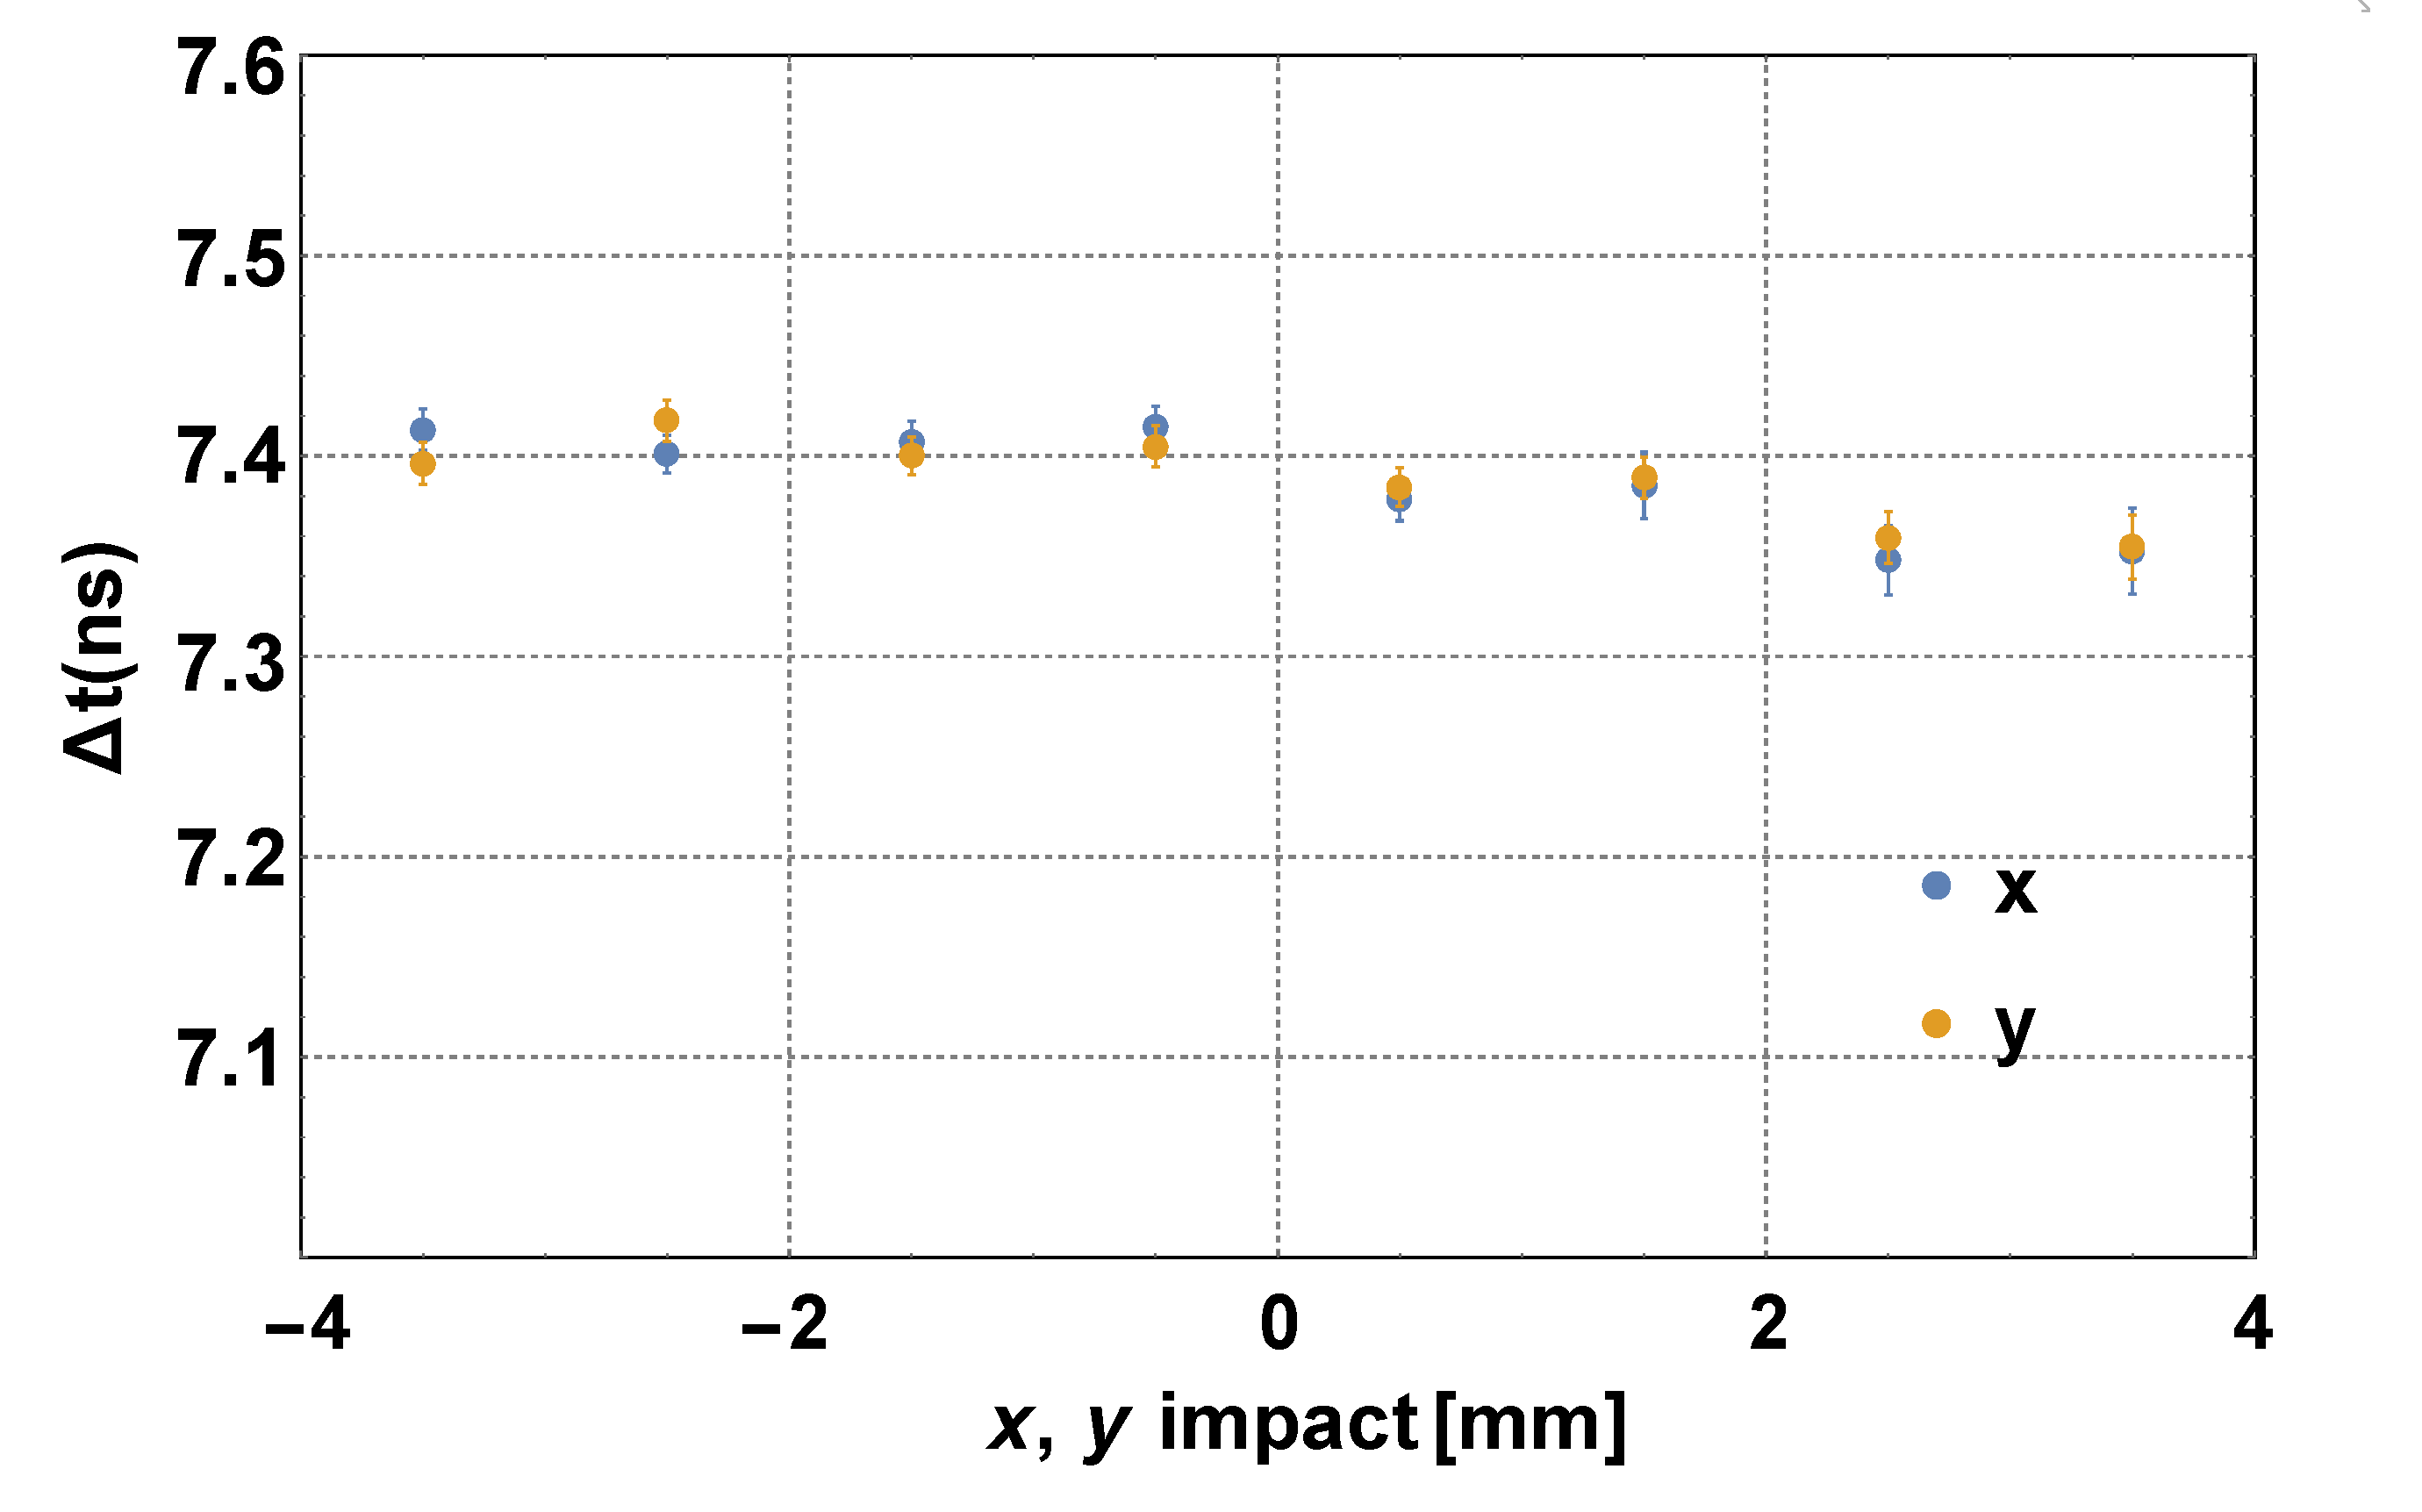
\includegraphics[width = 0.6 \textwidth]{toa8x8VsImpact}
  \caption{Average time of arrival as a function of impact position for a mesh readout APD. The measurement was performed using 150 GeV muons. The MCP PMT defines the origin of the time axis. The APD was operated at 1750 V, at a temperature of \textcolor{red}{...}$^\circ$C.}
  \label{fig:toa8x8impact}
\end{figure}

The dependence of the signal amplitude on the muons' impact position is shown in figure\,\ref{fig:ampli8x8impact}.
The figure shows the median amplitude obtained at different positions on the detector.
The amplitude shows small variations within the detector active area and falls within $\approx$200 $\mu$m from the detector edges ($\approx$4.5mm from the center).
\begin{figure}
  \centering
  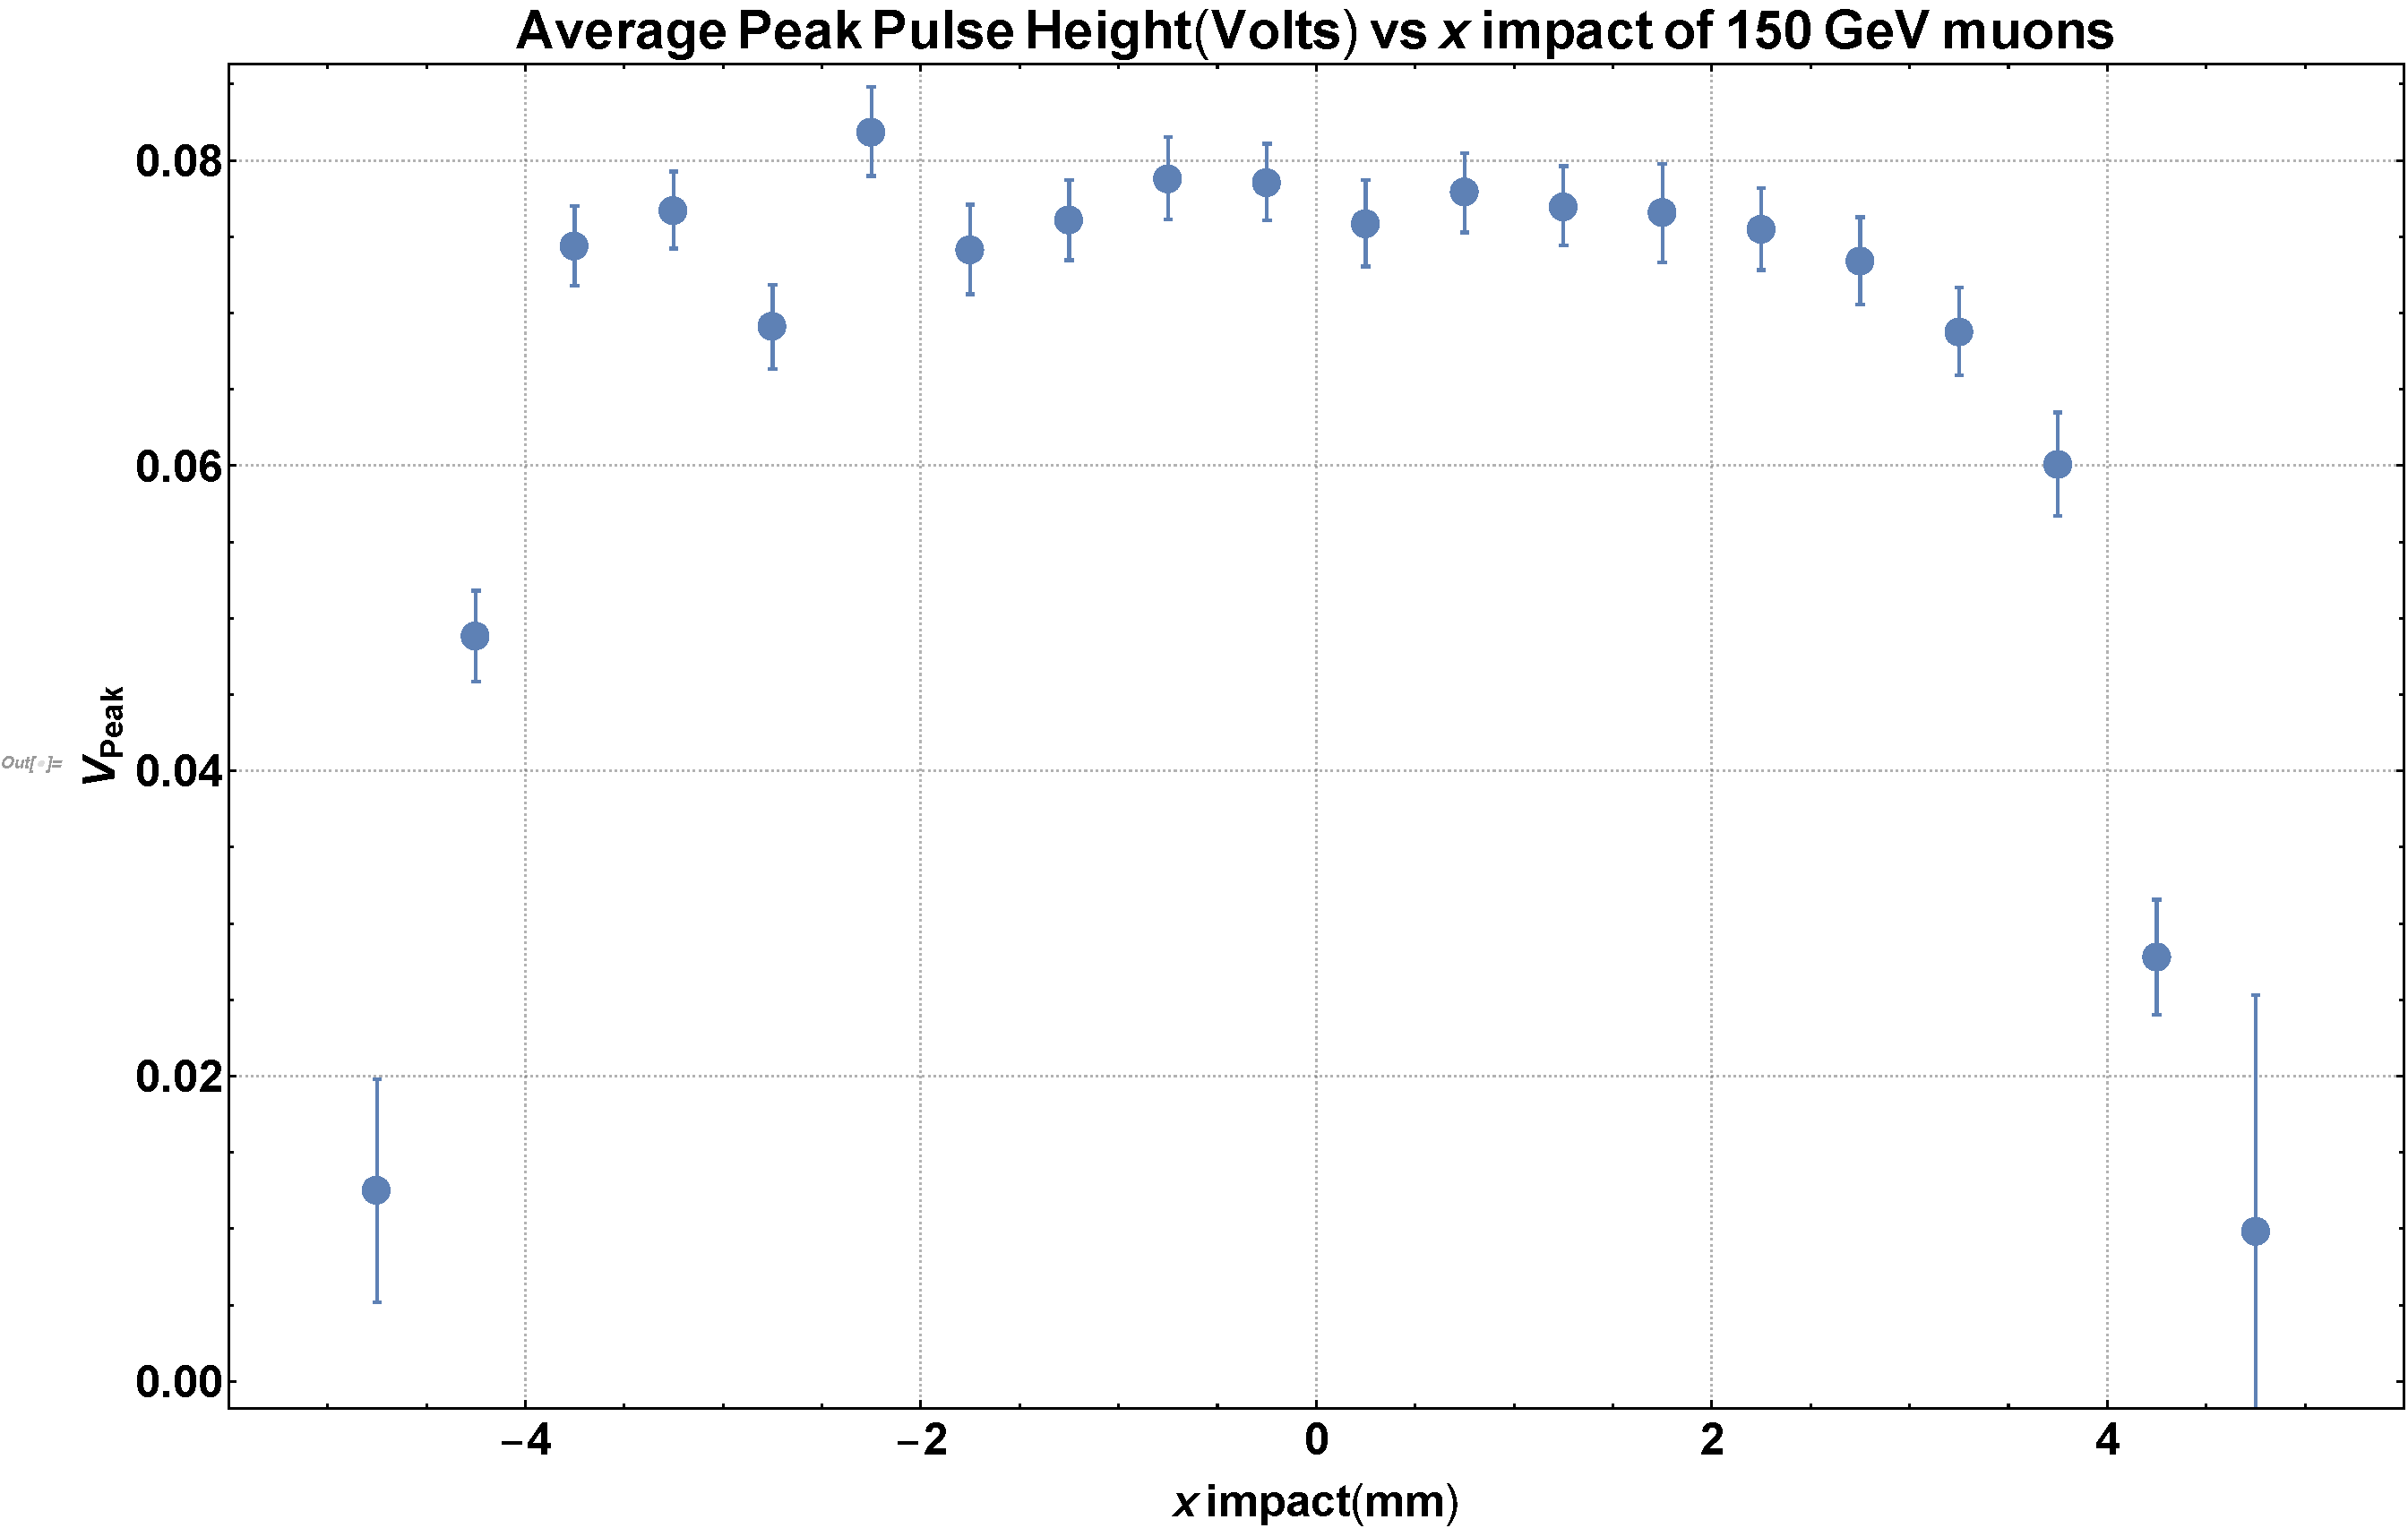
\includegraphics[width = 0.6 \textwidth]{ampli8x8vsImpact}
  \caption{Median amplitude as a function of impact position for a mesh readout APD. The measurement was performed using 150 GeV muons. The APD was operated at 1750 V, at a temperature of \textcolor{red}{...}$^\circ$C.}
  \label{fig:ampli8x8impact}
\end{figure}


\section{Summary}
\label{sec:summary}

For their operation at HL-LHC, the ATLAS and CMS experiments foresee timing systems for minimum ionising particles, aiming to a resolution around 30\,ps.
The detectors used in these systems will be subjected to fluences of up to $\Phi_{eq} = 10^{15}$\,cm$^{-2}$ for the goal integrated luminosity of HL-LHC of 3000\,fb$^{-1}$.

The parameters influencing the time resolution of deep diffused APDs with DC-coupled readout, as well as the uniformity of response of these devices, were measured.

Deep diffused APDs with an active area of $2 \times 2$\,mm$^2$ produced by RMD were irradiated with reactor neutrons up to a fluence of $\Phi_{eq} = 10^{15}$\,cm$^{-2}$.
The uniformity of response was studied using a pulsed infrared laser.
The sensitive area of the detectors is affected by irradiation, maintaining an uniform response at the centre of the sensors.
Current, amplitude, and timing characteristics of the detectors were measured at a temperature of $-20^\circ$C, before and after irradiation.
From the current-voltage characteristic it was found that the bulk current of the detectors increases with irradiation and that the gain decreases with irradiation.
The latter observation is supported by measurements of the APDs signal performed using a pulsed infrared laser shone at the centre of the detectors.
The time jitter of the APDs was determined using a pulsed infrared laser with an intensity corresponding to 0.8\,MIPs per pulse.
The laser was shone at the centre of the detectors.
The jitter is not degraded by exposure to fluences of up to at least $\Phi_{eq} = 6 \cdot 10^{13}$\,cm$^{-2}$.
The jitter of the device irradiated to $\Phi_{eq} = 3 \cdot 10^{14}$\,cm$^{-2}$ could not be determined due to its unstable behaviour, while the device irradiated to $\Phi_{eq} = 10^{15}$\,cm$^{-2}$ did not show any gain.

%These devices, with their current design, could be used as timing detectors in parts of the HL-LHC experiments where the fluences are in a range up to about $\Phi_{eq} = 10^{14}$\,cm$^{-2}$, with the upper bound to be studied with more detail than presented in this paper.

The uniformity of response of deep diffused APDs with an active area of $8 \times 8$\,mm$^2$ was studied using an infrared laser.
The amplitude of the signal shows a dependency on the distance between the point where the laser is shone and the electrical contact of the sensor.
The deposition of an aluminium layer on the detector surfaces improved the uniformity.
The timing characteristics of the metallised $8 \times 8$\,mm$^2$ APD were studied using a pulsed infrared laser with an intensity corresponding to 0.8\,MIPs per pulse.
The the time jitter was found to be 22\,ps at a voltage of 1750\,V.
The metallised sensors often shown instabilities when biased above 1700\,V.
The origin of these instabilities is under investigation.

Detectors with both DC- and AC-coupled readout will be characterised in beam tests to complement the information provided in this paper.
The determination of time resolution, uniformity of response, and detection efficiency are the aim of the beam tests.
The time resolution measurements with charged particles will include the \textit{Landau noise} term.
A comparison with the jitter obtained with infrared light will provide a direct measurement of how this effect influences the time resolution in these devices.

\textcolor{red}{The conclusions for the beam test and gain part have to be written}

\section*{Acknowledgments}

The work summarised in this paper has been performed within the framework of the RD50 collaboration.
This project has received funding from the European Union’s Horizon 2020 Research and Innovation programme under Grant Agreement no.\ 654168.
The authors wish to thank J.~Bronuzzi for the help during the clean room operations and in the development of the recipe for the metallisation of the devices.
The authors are grateful to the members of the CERN EP-DT-DD SSD team that developed and maintain the setups used in this work.

\bibliographystyle{ieeetr}
%\bibliographystyle{alpha}
\bibliography{bibliography}

\end{document}

\begin{figure}
  \centering
  \includegraphics[width = 0.6 \textwidth]{}
  \caption{}
  \label{fig:}
\end{figure}

\begin{figure}
  \centering
  \subfloat[]{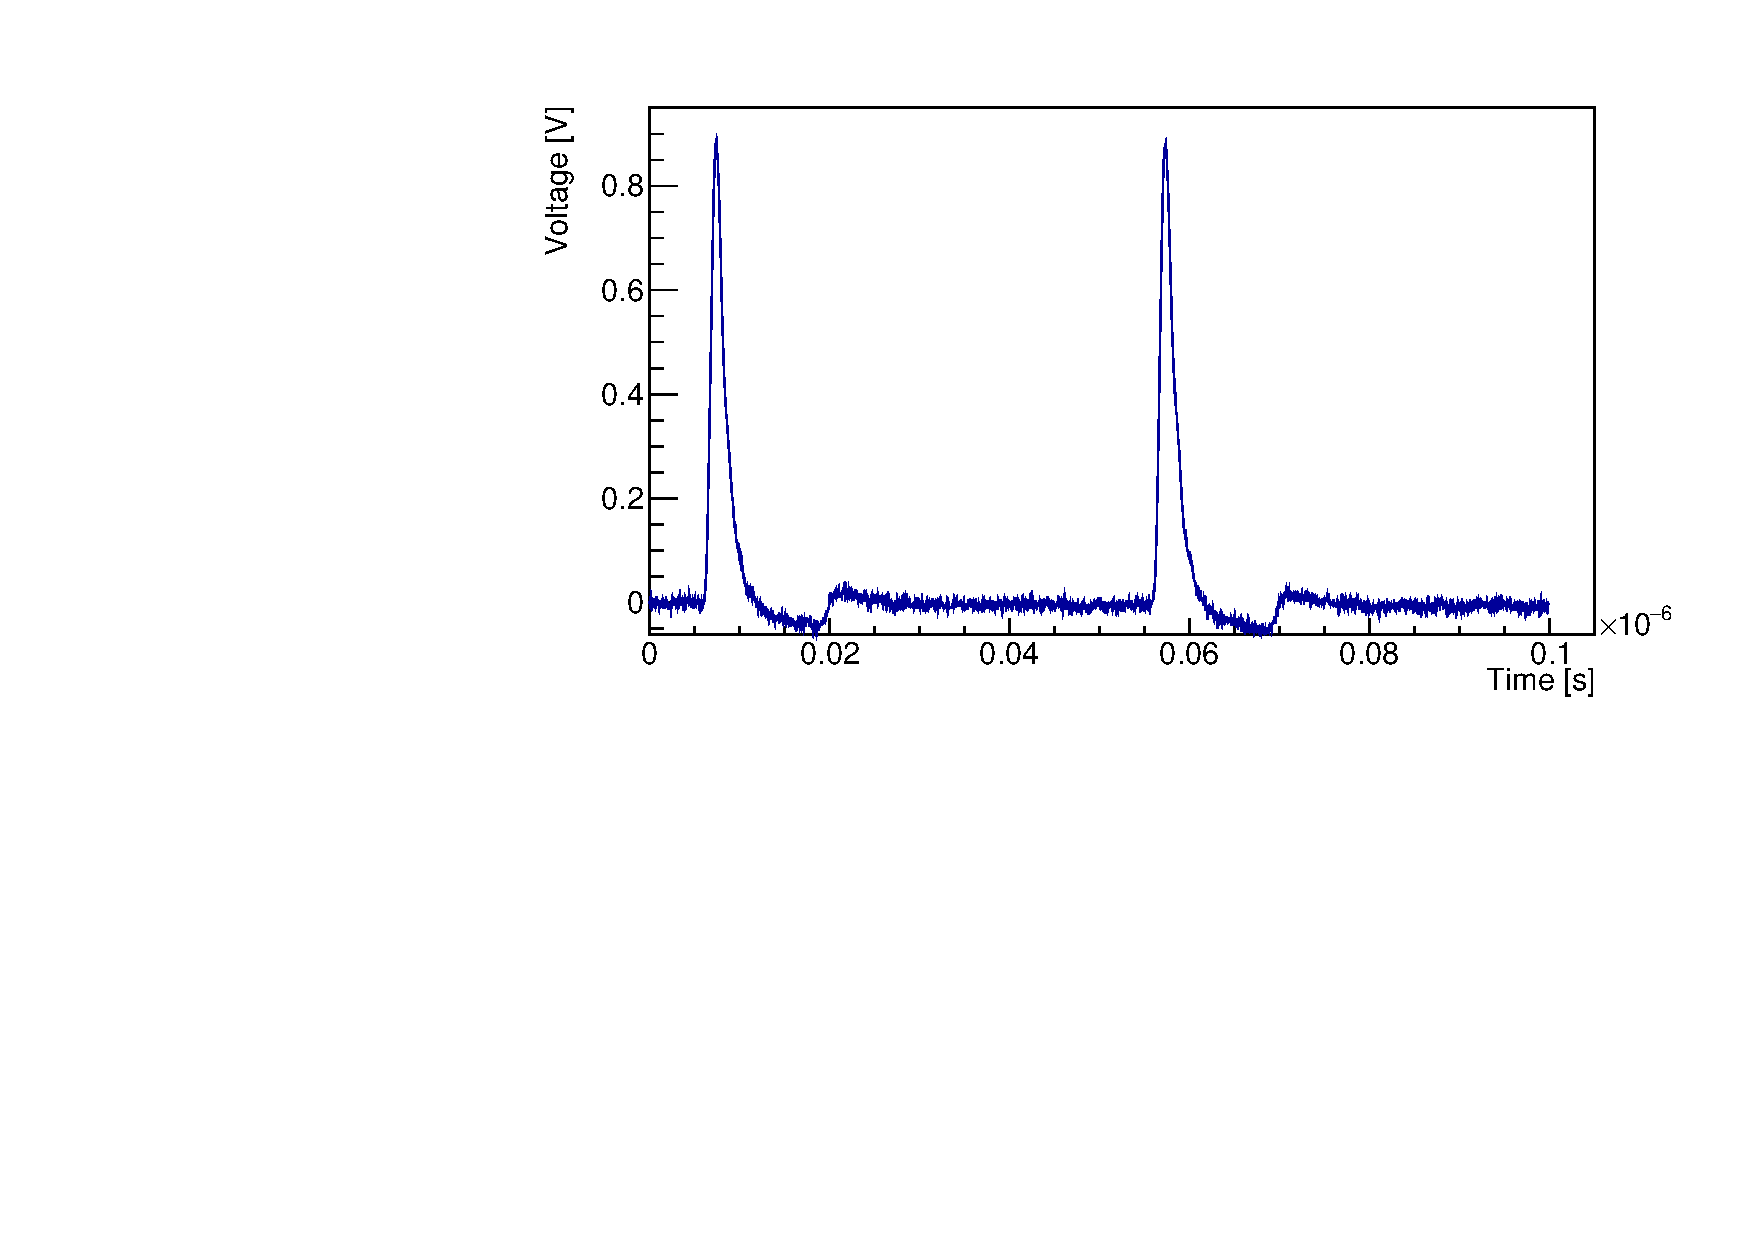
\includegraphics[width = 0.5 \textwidth]{APD_394-1-51_1665V_evt1100_2pulses}}\\
  \subfloat[]{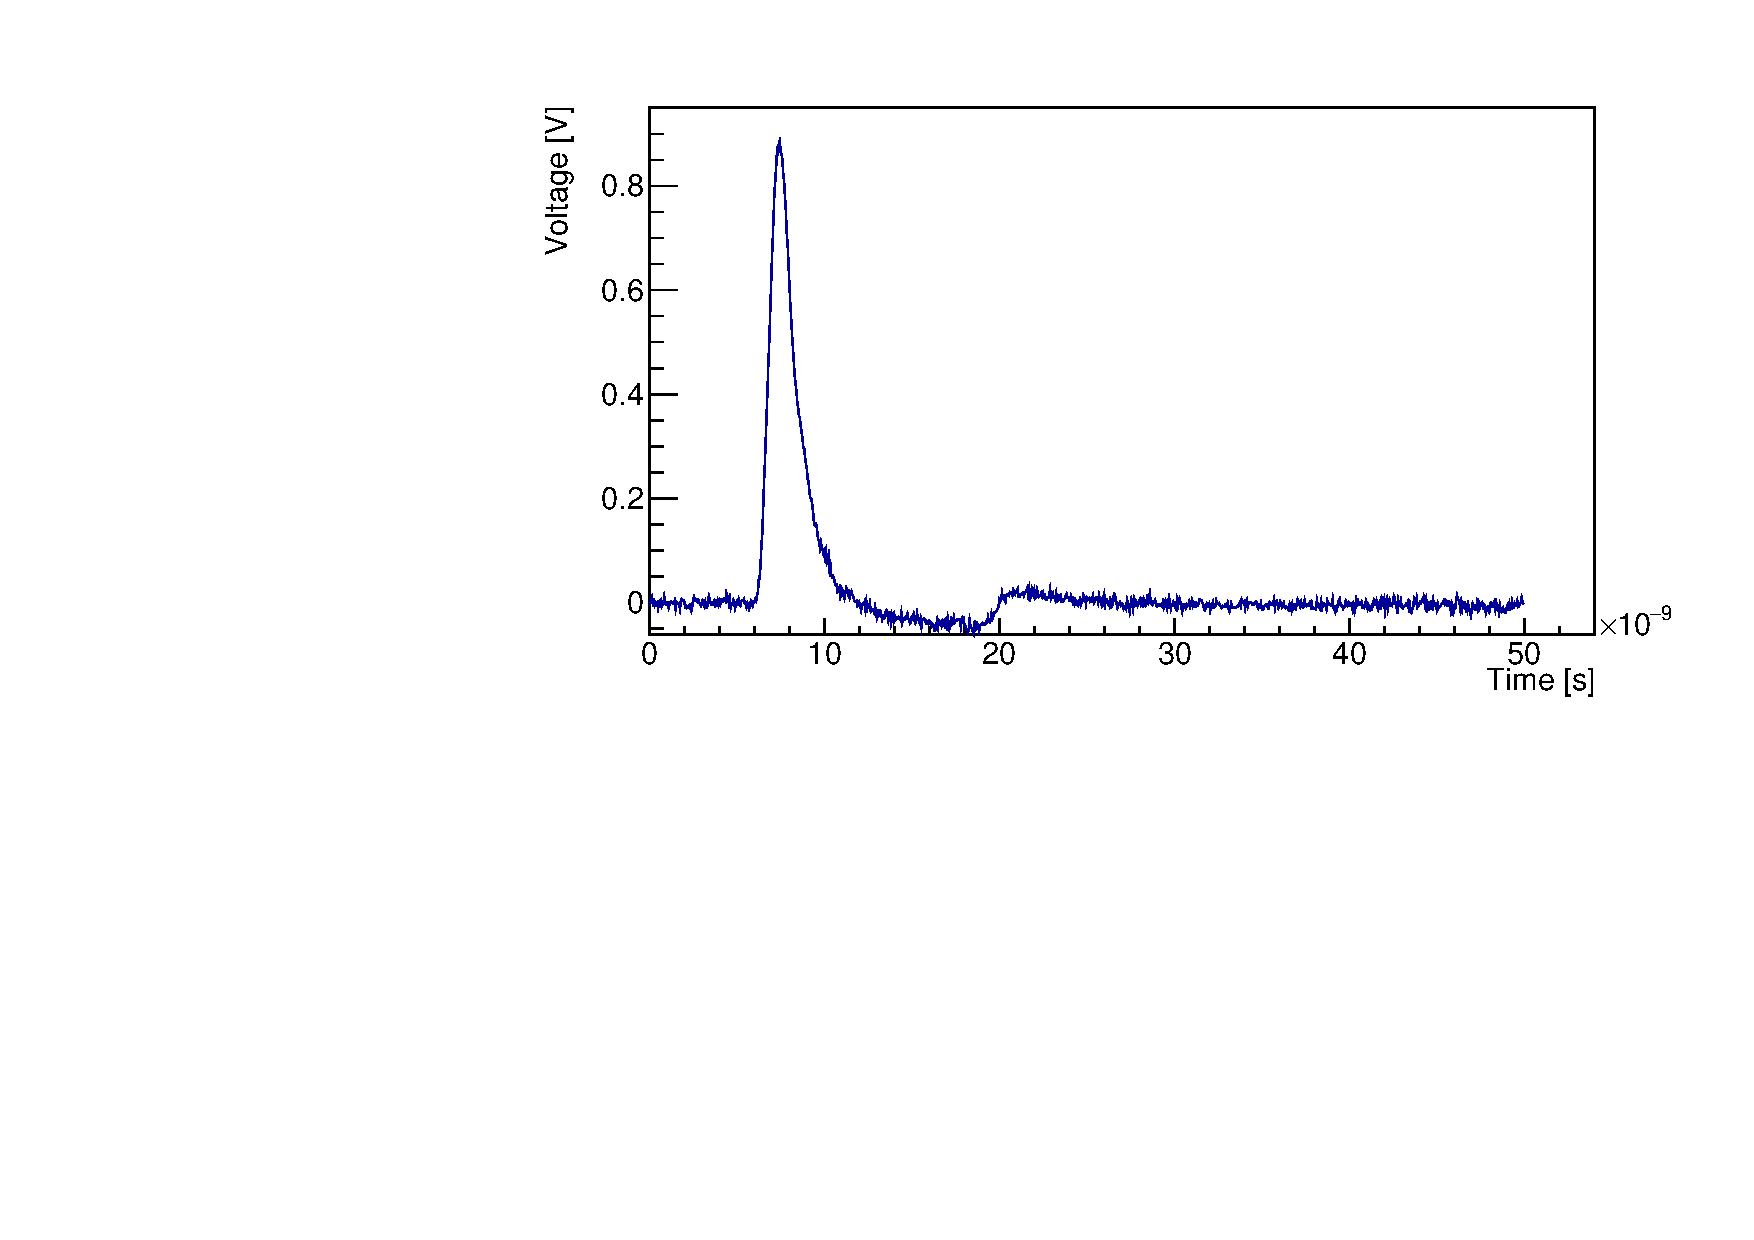
\includegraphics[width = 0.45 \textwidth]{APD_394-1-51_1665V_evt1100_firstPulse}}
  \hfill
  \subfloat[]{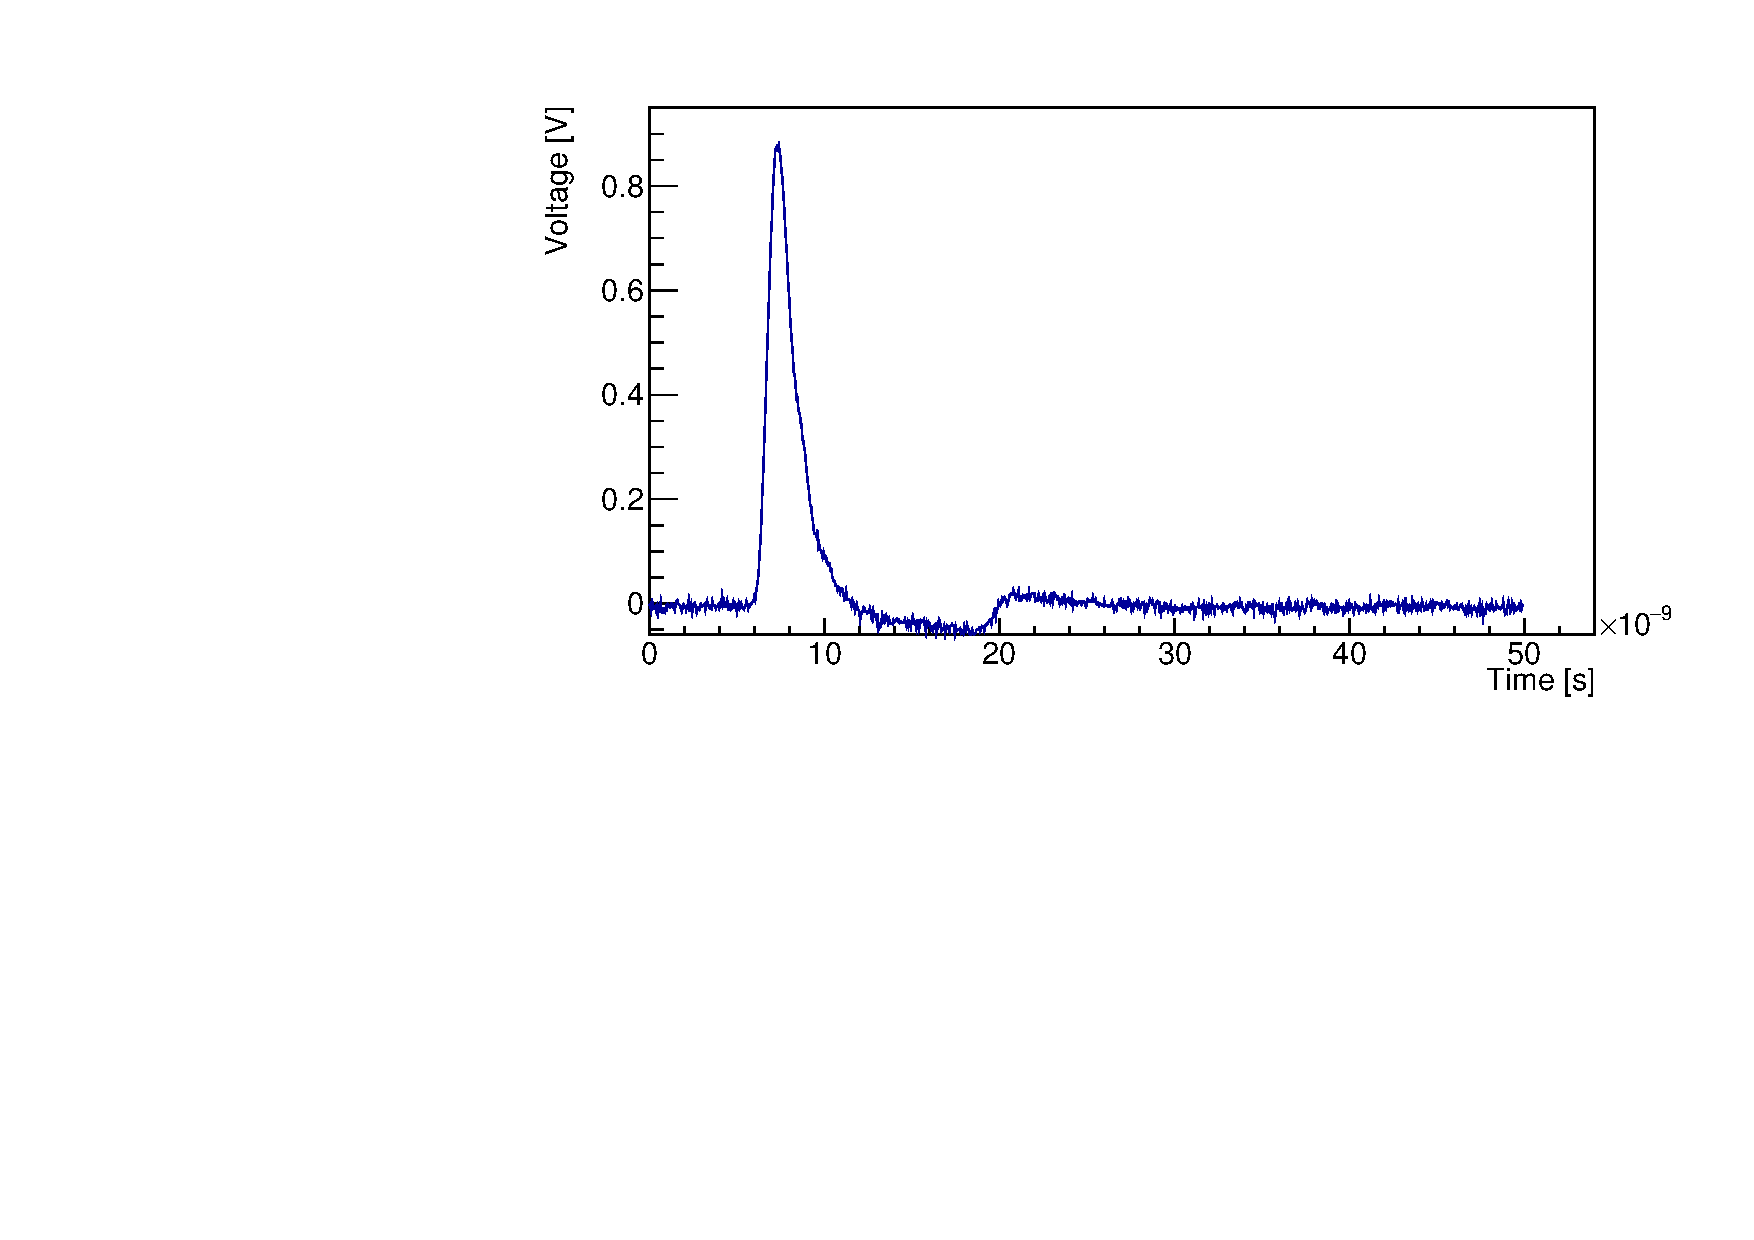
\includegraphics[width = 0.45 \textwidth]{APD_394-1-51_1665V_evt1100_secondPulse}}
  \caption{}
  \label{fig:pulses2x2timing}
\end{figure}
